\title{Buku Tugas Akhir ITS}
\author{Musk, Elon Reeve}
% Pengaturan ukuran teks dan bentuk halaman dua sisi
\documentclass[12pt,twoside]{report}
% Pengaturan ukuran halaman dan margin
\usepackage[a4paper,top=30mm,left=30mm,right=20mm,bottom=25mm]{geometry}
\usepackage[table,xcdraw]{xcolor}

\usepackage[english]{babel}
% Pengaturan pewarnaan

%\usepackage{colortbl} 
\usepackage[utf8]{inputenc}
\usepackage{amsmath}
\usepackage{multirow} % for multirow command
% Pengaturan ukuran spasi
\usepackage[singlespacing]{setspace}
\usepackage{rotating} % for sidewaystable environment
\usepackage[ruled,vlined]{algorithm2e} % for algorithm2e environment
\usepackage{pdflscape} % for landscape environment
\usepackage{hyphenat} % for \nohyphens command
% Pengaturan detail pada file PDF
\usepackage[pdfauthor={\@author},bookmarksnumbered,pdfborder={0 0 0}]{hyperref}

% Pengaturan jenis karakter
\usepackage[utf8]{inputenc}


% Pengaturan kutipan artikel
%\usepackage[style=ieee, backend=biber]{biblatex}

% Package lainnya
\usepackage{changepage}
\usepackage{enumitem}
\usepackage{eso-pic}
\usepackage{txfonts} % Font times
\usepackage{etoolbox}
\usepackage{graphicx}
\usepackage{lipsum}
\usepackage{caption}
\usepackage{longtable}


\usepackage{tabularx}
\usepackage{wrapfig}
\usepackage{float}
\usepackage{array} % Add this line in the preamble
\usepackage{ifthen}
\usepackage{etoolbox}
\usepackage{cite}

% Add your bibliography file
%\addbibresource{pustaka/pustaka.bib}

% Define boolean variables

%\captionsetup[longtable]{
%  width=.9\textwidth, % Adjust the width to .9 of the text width or as needed
%}

% Definisi untuk "Hati ini sengaja dikosongkan"
\patchcmd{\cleardoublepage}{\hbox{}}{
  \thispagestyle{empty}
  \vspace*{\fill}
  \begin{center}\textit{[Halaman ini sengaja dikosongkan]}\end{center}
  \vfill}{}{}

% Pengaturan penomoran halaman
\usepackage{fancyhdr}
\fancyhf{}
\renewcommand{\headrulewidth}{0pt}
\pagestyle{fancy}
\fancyfoot[LE,RO]{\thepage}
\patchcmd{\chapter}{plain}{fancy}{}{}
\patchcmd{\chapter}{empty}{plain}{}{}

% Command untuk bulan
\newcommand{\MONTH}{%
  \ifcase\the\month
  \or Januari% 1
  \or Februari% 2
  \or Maret% 3
  \or April% 4
  \or Mei% 5
  \or Juni% 6
  \or Juli% 7
  \or Agustus% 8
  \or September% 9
  \or Oktober% 10
  \or November% 11
  \or Desember% 12
  \fi}
\newcommand{\ENGMONTH}{%
  \ifcase\the\month
  \or January% 1
  \or February% 2
  \or March% 3
  \or April% 4
  \or May% 5
  \or June% 6
  \or July% 7
  \or August% 8
  \or September% 9
  \or October% 10
  \or November% 11
  \or December% 12
  \fi}

% Pengaturan format judul bab
\usepackage{titlesec}
\titleformat{\chapter}[display]{\bfseries\Large}{BAB \centering\Roman{chapter}}{0ex}{\vspace{0ex}\centering}
\titleformat{\section}{\bfseries\large}{\MakeUppercase{\thesection}}{1ex}{\vspace{1ex}}
\titleformat{\subsection}{\bfseries\large}{\MakeUppercase{\thesubsection}}{1ex}{}
\titleformat{\subsubsection}{\bfseries\large}{\MakeUppercase{\thesubsubsection}}{1ex}{}
\titlespacing{\chapter}{0ex}{0ex}{4ex}
\titlespacing{\section}{0ex}{1ex}{0ex}
\titlespacing{\subsection}{0ex}{0.5ex}{0ex}
\titlespacing{\subsubsection}{0ex}{0.5ex}{0ex}
\setcounter{secnumdepth}{3} % Untuk memberi penomoran pada \subsubsection
\newcommand{\engtatitle}{dadfa}

\newcommand{\NamaMahasiswa}[2]{
	\newcommand{\name}{#1}
	\newcommand{\nrp}{#2}

}

\newcommand{\JudulTAInd}[1]{
	\newcommand{\tatitle}{#1}
}
\newcommand{\JudulTAEng}[1]{
			\renewcommand{\engtatitle}{#1}
	}
	
\newcommand{\Tempat}[1]{
		%Surabaya
		\newcommand{\place}{#1}

	}




\newbool{bpembimbing2}
\newbool{bpenguji3}
\setbool{bpembimbing2}{false}
\setbool{bpenguji3}{false}



\newcommand{\PembimbingSatu}[2]{
\newcommand{\advisor}{#1}
\newcommand{\advisornip}{#2}
} 
\newcommand{\PembimbingDua}[2]{
\newcommand{\coadvisor}{#1}
\newcommand{\coadvisornip}{#2}
\setbool{bpembimbing2}{true}
}


\newcommand{\PengujiSatu}[2]{
\newcommand{\examinerone}{#1}
\newcommand{\examineronenip}{#2}

} 

\newcommand{\PengujiDua}[2]{
\newcommand{\examinertwo}{#1}
\newcommand{\examinertwonip}{#2}

} 

\newcommand{\PengujiTiga}[2]{
\newcommand{\examinerthree}{#1}
\newcommand{\examinerthreenip}{#2}

\setbool{bpenguji3}{true}

}

\newcommand{\KepalaDepartemen}[2]{
\newcommand{\headofdepartment}{#1}
\newcommand{\headofdepartmentnip}{#2}
} 



% jurusan\
\newcommand{\Departemen}[2]{
\newcommand{\studyprogram}{#1}
\newcommand{\engstudyprogram}{#2}
\newcommand{\department}{#1}
\newcommand{\engdepartment}{#2}
}

% fakultas
\newcommand{\Fakultas}[2]{
\newcommand{\faculty}{#1}
\newcommand{\engfaculty}{#2}
}
% singkatan fakultas
\newcommand{\SingkatanFakultas}[2]{
\newcommand{\facultyshort}{#1}
\newcommand{\engfacultyshort}{#2}
}

% departemen

% kode mata kuliah
\newcommand{\KodeMataKuliah}[1]{
\newcommand{\coursecode}{#1}
}



%\input{pustaka/variables.tex}

% Tambahkan format tanda hubung yang benar di sini
\hyphenation{
  ro-ket
  me-ngem-bang-kan
  per-hi-tu-ngan
  tek-no-lo-gi
  me-la-ku-kan
  ber-so-si-al-i-sa-si
  me-nge-na-i
}



% Pengaturan format potongan kode
\usepackage{listings}
\definecolor{comment}{RGB}{0,128,0}
\definecolor{string}{RGB}{255,0,0}
\definecolor{keyword}{RGB}{0,0,255}
\lstdefinestyle{codestyle}{
  commentstyle=\color{comment},
  stringstyle=\color{string},
  keywordstyle=\color{keyword},
  basicstyle=\footnotesize\ttfamily,
  numbers=left,
  numberstyle=\tiny,
  numbersep=5pt,
  frame=lines,
  breaklines=true,
  prebreak=\raisebox{0ex}[0ex][0ex]{\ensuremath{\hookleftarrow}},
  showstringspaces=false,
  upquote=true,
  tabsize=2,
}
\lstset{style=codestyle}
\usepackage{array}
\usepackage{tikz}
\usetikzlibrary{shapes.geometric, arrows.meta, positioning}
%========================================
%Template ini di modifikasi oleh departement Teknik Komputer ITS
%dari template yang telah dibuat Musk, Elon Reeve
%=======================================

%=======================================
%Direktori Penting 
%1. Init : Berisi File penting terkait dengan konfigurasi .
%            Isi dari direktori ini jangan diubah
%2.KataPengantar 
%3. Abstrak : berisi abstrak untuk bahasa indonesia dan bahasa inggris 
%4. Bab1-Bab5 : Isi tiap-tiap bab
%5. Pustaka : Berisi daftar pustaka 
%6. Biografi penulis 
%=======================================

%========================================
% Identitas Mahasiswa} 
%========================================
\NamaMahasiswa{I Putu Deva Febriana}{5024 21 1016}

%========================================
%Identitas Tugas Akhir
%========================================
\KodeMataKuliah{EC234801}
\JudulTAInd{PENGEMBANGAN SISTEM KENDALI KURSI RODA BERBASIS \emph{SIBI} DAN \emph{BRAKING SYSTEM} MENGGUNAKAN \emph{LSTM} dan \emph{YOLOv11}}
\JudulTAEng{DEVELOPMENT OF WHEELCHAIR CONTROL SYSTEM BASED ON SIBI AND BRAKING SYSTEM USING LSTM AND YOLOv11}
\Tempat{Surabaya}

%========================================
% Daftar Pembimbing 
%========================================
\PembimbingSatu{Dr. Supeno Mardi Susiki Nugroho,S.T.,M.T.}{19700313199512 1 001} 
\PembimbingDua{Dr. Eko Mulyanto Yuniarno,S.T.,M.T.}{19680601199512 1 009 } 

%========================================
% Daftar Penguji
%========================================
\PengujiSatu{Prof. Dr. I Ketut Eddy Purnama, S.T., M.T.}{19690730199512 1 001} 
\PengujiDua{Dr. Susi Juniastuti, S.T., M.Eng.}{19650618199903 2 001}
\PengujiTiga{Dr. Surya Sumpeno , S.T., M.Sc.} {19690613199702 1 003}



%========================================
%Identitas Departement dan fakultas
%========================================
\KepalaDepartemen{Dr. Arief Kurniawan, S.T., M.T.}{19740907200212 1 001} 
\Departemen{Teknik Komputer}{Computer Engineering}
\Fakultas{Teknologi Elektro dan Informatika Cerdas}{Intelligent Electrical And Informatics Technology}
\SingkatanFakultas{FTEIC}{FIEI}


% Isi keseluruhan dokumen
\begin{document}

\AddToShipoutPictureBG*{
  \AtPageLowerLeft{
    % Ubah nilai berikut jika posisi horizontal background tidak sesuai
    \hspace{-3.25mm}
c
    % Ubah nilai berikut jika posisi vertikal background tidak sesuai
    \raisebox{0mm}{
      
\includegraphics[width=\paperwidth,height=\paperheight]{Init/gambar/sampul-luar.png}
    }
  }
}

% Menyembunyikan nomor halaman
\thispagestyle{empty}

% Pengaturan margin untuk menyesuaikan konten sampul
\newgeometry{
  top=55mm,
  left=30mm,
  right=20mm,
  bottom=20mm
}

\begin{flushleft}

  % Pemilihan font sans serif
  \sffamily

  % Pemilihan warna font putih
  \color{white}

  % Pemilihan font bold
  \fontseries{bx}
  \selectfont
  \begin{spacing}{1.5}
   \begin{large}
  TUGAS AKHIR - \coursecode{}
\end{large}

\vspace{\fill}

\begin{spacing}{1.5}
  \begin{Large}
    \tatitle{}
  \end{Large}
\end{spacing}

\vspace{\fill}

\begin{large}
  \name{} \\
  \textmd{NRP \nrp{}}
\end{large}

\vspace{\fill}

\begin{large}
  \textmd{Dosen Pembimbing} \\
  \advisor{} \\
  \textmd{NIP \advisornip{}} \\
  \coadvisor{} \\
  \textmd{NIP \coadvisornip{}}
\end{large}

\vspace{\fill}

Program Studi Strata 1 (S1) \studyprogram{} \\

\mdseries

Departemen \department{} \\
Fakultas \faculty{} \\
Institut Teknologi Sepuluh Nopember

\place{} \\ \the\year{}

  \end{spacing}

\end{flushleft}

\restoregeometry

\cleardoublepage

% Atur ulang penomoran halaman
\setcounter{page}{1}

% Sampul dalam Bahasa Indonesia
\AddToShipoutPictureBG*{
  \AtPageLowerLeft{
    % Ubah nilai berikut jika posisi horizontal background tidak sesuai
    \hspace{-4mm}

    % Ubah nilai berikut jika posisi vertikal background tidak sesuai
    \raisebox{0mm}{
      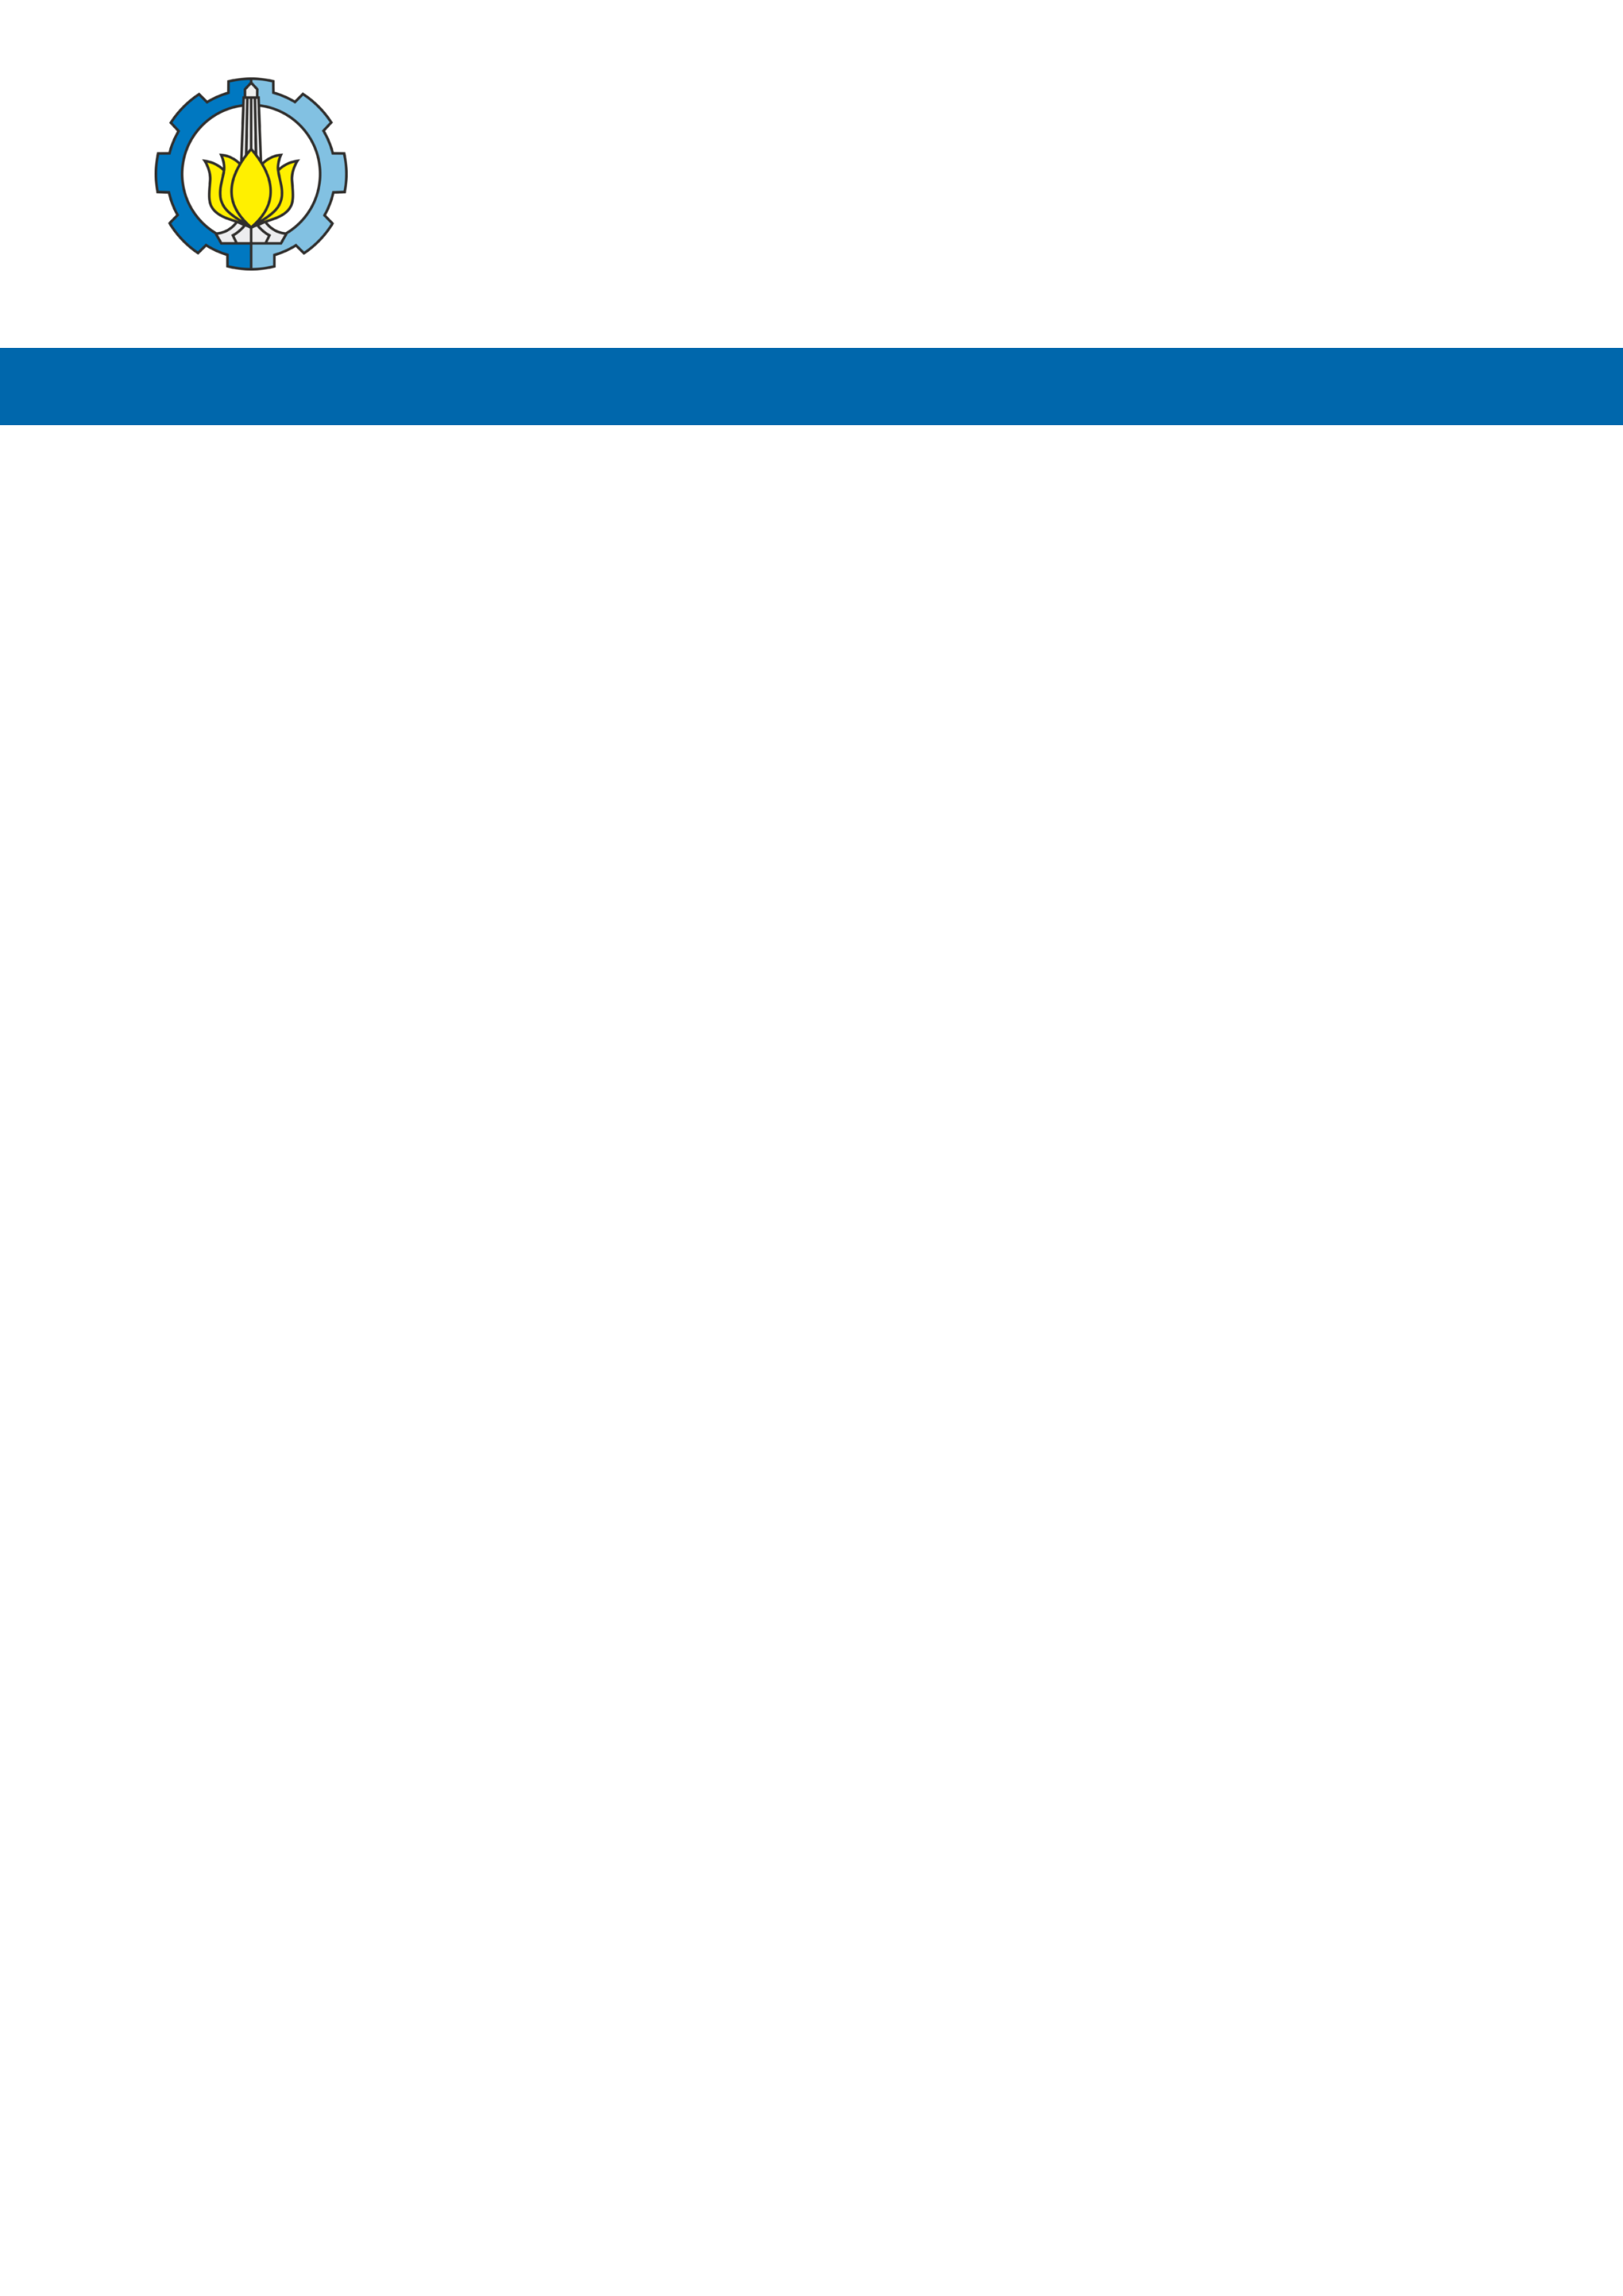
\includegraphics[width=\paperwidth,height=\paperheight]{Init/gambar/sampul-luar-tipis.png}
    }
  }
}

% Menyembunyikan nomor halaman
\thispagestyle{empty}

% Pengaturan margin untuk menyesuaikan konten sampul
\newgeometry{
  top=65mm,
  left=30mm,
  right=30mm,
  bottom=20mm
}

\begin{flushleft}

  % Pemilihan font sans serif
  \sffamily

  % Pemilihan font bold
  \fontseries{bx}
  \selectfont
  \begin{spacing}{1.5}
\begin{large}
  TUGAS AKHIR - \coursecode{}
\end{large}

\vspace{\fill}

\begin{spacing}{1.5}
  \begin{Large}
    \tatitle{}
  \end{Large}
\end{spacing}

\vspace{\fill}

\begin{large}
  \name{} \\
  \textmd{NRP \nrp{}}
\end{large}

\vspace{\fill}

\begin{large}
  \textmd{Dosen Pembimbing} \\
  \advisor{} \\
  \textmd{NIP \advisornip{}} \\
  \coadvisor{} \\
  \textmd{NIP \coadvisornip{}}
\end{large}

\vspace{\fill}

Program Studi Strata 1 (S1) \studyprogram{} \\

\mdseries

Departemen \department{} \\
Fakultas \faculty{} \\
Institut Teknologi Sepuluh Nopember

\place{} \\ \the\year{}

  \end{spacing}

\end{flushleft}

\restoregeometry

\clearpage
\cleardoublepage

% Sampul dalam Bahasa Inggris

\AddToShipoutPictureBG*{
  \AtPageLowerLeft{
    % Ubah nilai berikut jika posisi horizontal background tidak sesuai
    \hspace{-4mm}

    % Ubah nilai berikut jika posisi vertikal background tidak sesuai
    \raisebox{0mm}{
      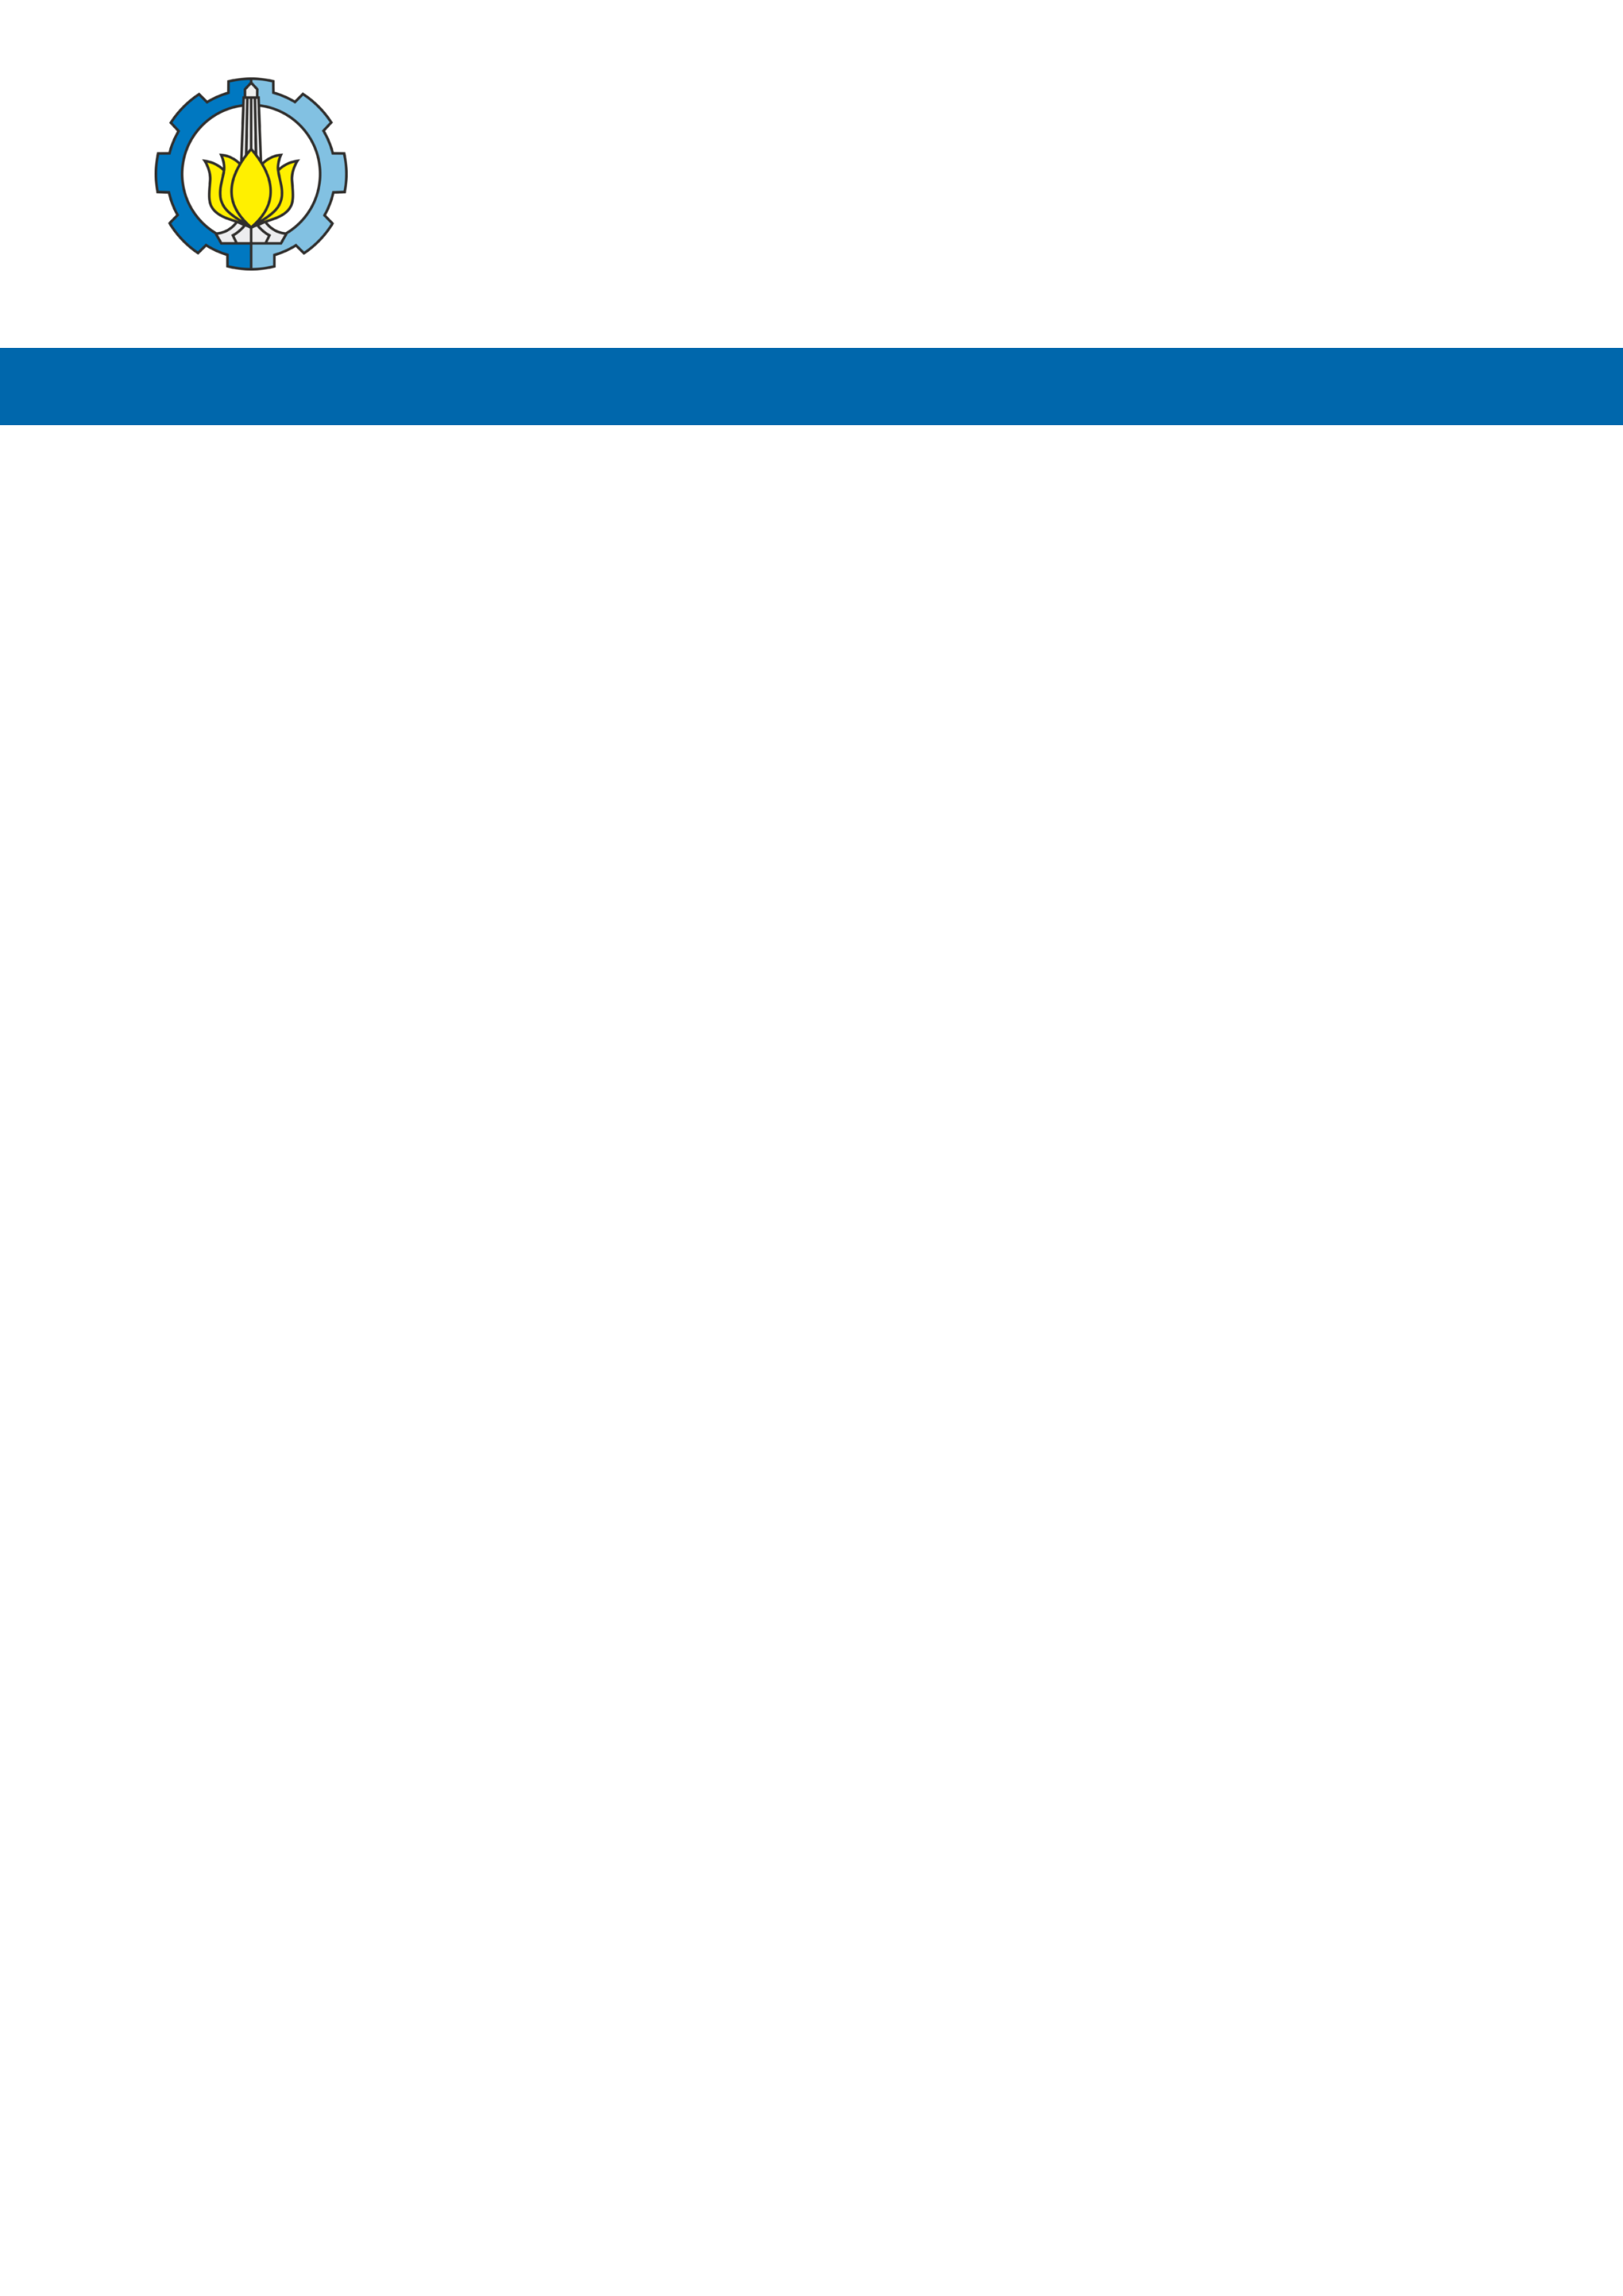
\includegraphics[width=\paperwidth,height=\paperheight]{Init/gambar/sampul-luar-tipis.png}
    }
  }
}

% Menyembunyikan nomor halaman
\thispagestyle{empty}

% Pengaturan margin untuk menyesuaikan konten sampul
\newgeometry{
  top=65mm,
  left=30mm,
  right=30mm,
  bottom=20mm
}

\begin{flushleft}

  % Pemilihan font sans serif
  \sffamily

  % Pemilihan font bold
  \fontseries{bx}
  \selectfont
  \begin{spacing}{1.5}
   \begin{large}
  FINAL PROJECT - \coursecode{}
\end{large}

\vspace{\fill}

\begin{spacing}{1.5}
  \begin{Large}
    \engtatitle{}
  \end{Large}
\end{spacing}

\vspace{\fill}

\begin{large}
  \name{} \\
  \textmd{NRP \nrp{}}
\end{large}

\vspace{\fill}

\begin{large}
  \textmd{Advisor} \\
  \advisor{} \\
  \textmd{NIP \advisornip{}} \\
  \coadvisor{} \\
  \textmd{NIP \coadvisornip{}}
\end{large}

\vspace{\fill}

Undergraduate Study Program of \engstudyprogram{} \\

\mdseries

Department of \engdepartment{} \\
Faculty of \engfaculty{} \\
Sepuluh Nopember Institute of Technology

\place{} \\ \the\year{}

  \end{spacing}

\end{flushleft}

\restoregeometry

\cleardoublepage

% Label tabel dan gambar dalam bahasa indonesia
\renewcommand{\figurename}{Gambar}
\renewcommand{\tablename}{Tabel}

% Pengaturan ukuran indentasi paragraf
\setlength{\parindent}{2em}

% Pengaturan ukuran spasi paragraf
\setlength{\parskip}{1ex}

% Lembar pengesahan
\begin{center}
	\large
  \textbf{LEMBAR PENGESAHAN}
\end{center}
\thispagestyle{empty}

\begin{center}
  % Ubah kalimat berikut dengan judul tugas akhir
  \textbf{PENGEMBANGAN SISTEM KENDALI KURSI RODA BERBASIS \emph{SIBI} DAN \emph{BRAKING SYSTEM} MENGGUNAKAN \emph{LSTM} dan \emph{YOLOv11}}
\end{center}

\begingroup
% Pemilihan font ukuran small
\small

\begin{center}
  % Ubah kalimat berikut dengan pernyataan untuk lembar pengesahan
  \textbf{PROPOSAL TUGAS AKHIR} \\
  Diajukan untuk memenuhi salah satu syarat memperoleh gelar
  Sarjana Teknik pada
  Program Studi S-1 Teknik Komputer \\
  Departemen Teknik Komputer \\
  Fakultas Teknik Elektro dan Informatika Cerdas \\
  Institut Teknologi Sepuluh Nopember
\end{center}

\begin{center}
  % Ubah kalimat berikut dengan nama dan NRP mahasiswa
  Oleh: \textbf{I Putu Deva Febriana} \\
  NRP. 5024211016
\end{center}

\begin{center}
  Disetujui Oleh:
\end{center}

\vspace{3ex}

\begingroup
% Menghilangkan padding
\setlength{\tabcolsep}{0pt}

\noindent
    \begin{tabularx}{\textwidth}{X c}
      % Ubah kalimat-kalimat berikut dengan nama dan NIP dosen pembimbing pertama
      Dr. Supeno Mardi Susiki Nugroho,S.T.,M.T.          & (Pembimbing 1) \\
      NIP: 19700313199512 1 001       & \\
      &  \\
      &  \\
      % Ubah kalimat-kalimat berikut dengan nama dan NIP dosen pembimbing kedua
      Dr. Eko Mulyanto Yuniarno,S.T.,M.T.     & (Pembimbing 2) \\
      NIP: 19680601199512 1 009       & \\
      &  \\
      &  \\
      % Ubah kalimat-kalimat berikut dengan nama dan NIP dosen penguji pertama
      Prof. Dr. I Ketut Eddy Purnama, S.T., M.T.  & (Penguji I) \\
      NIP: 19690730199512 1 001       & \\
      &  \\
      &  \\
      % Ubah kalimat-kalimat berikut dengan nama dan NIP dosen penguji kedua
      Dr. Susi Juniastuti, S.T., M.Eng.  & (Penguji II) \\
      NIP : 19650618199903 2 001       & \\
      &  \\
      &  \\
      % Ubah kalimat-kalimat berikut dengan nama dan NIP dosen penguji ketiga
      Dr. Surya Sumpeno , S.T., M.Sc.            & (Penguji III) \\
      NIP: 19690613199702 1 003        & \\
    \end{tabularx}
\endgroup
\vspace{2ex}
\begin{center}
    Mengetahui,\\
  % Ubah kalimat berikut dengan nama departemen
  Kepala Departemen Teknik Komputer, FTEIC\\
  \vspace{10ex}
  % Ubah kalimat berikut dengan jabatan kepala departemen
  \underline{Dr. Arief Kurniawan, S.T., M.T. }\\
  NIP: 19740907200212 1 001 \\
  \vspace{10ex}
  % Ubah text dibawah menjadi tempat dan tanggal
  \textbf{SURABAYA} \\
  \textbf{Februari, 2025}
\end{center}
\endgroup
\cleardoublepage
\begin{center}
	\large
  \textbf{APPROVAL SHEET}
\end{center}

% Menyembunyikan nomor halaman
\thispagestyle{empty}

\begin{center}
  % Ubah kalimat berikut dengan judul tugas akhir
  \textbf{DEVELOPMENT OF WHEELCHAIR CONTROL SYSTEM BASED ON SIBI AND BRAKING SYSTEM USING LSTM AND YOLOv11}
\end{center}

\begingroup
  % Pemilihan font ukuran small
  \small

  \begin{center}
    % Ubah kalimat berikut dengan pernyataan untuk lembar pengesahan
    \textbf{FINAL PROJECT PROPOSAL} \\
    Submitted to fulfill one of the requirements for obtaining a degree
    Bachelor of Engineering at 
    Undergraduate Study Program of Computer Engineering \\
    Department of Computer Engineering \\
    Faculty of Intelligent Electrical and Informatics Technology \\
    Sepuluh Nopember Institute of Technology
  \end{center}

  \begin{center}
    % Ubah kalimat berikut dengan nama dan NRP mahasiswa
    By: \textbf{I Putu Deva Febriana} \\
    NRP. 5024211016
  \end{center}

  \begin{center}
    Approved by Final Project Proposal Examiner Team:
  \end{center}
 \vspace{3ex}
  \begingroup
    % Menghilangkan padding
    \setlength{\tabcolsep}{0pt}

    \noindent
    \begin{tabularx}{\textwidth}{X c}
      % Ubah kalimat-kalimat berikut dengan nama dan NIP dosen pembimbing pertama
      Dr. Supeno Mardi Susiki Nugroho,S.T.,M.T.          & (Advisor 1) \\
      NIP: 19700313199512 1 001       & \\
      &  \\
      &  \\
      % Ubah kalimat-kalimat berikut dengan nama dan NIP dosen pembimbing kedua
      Dr. Eko Mulyanto Yuniarno,S.T.,M.T.     & (Advisor 2) \\
      NIP: 19680601199512 1 009       & \\
      &  \\
      &  \\
      % Ubah kalimat-kalimat berikut dengan nama dan NIP dosen penguji pertama
      Prof. Dr. I Ketut Eddy Purnama, S.T., M.T.  & (Examiner I) \\
      NIP: 19690730199512 1 001       & \\
      &  \\
      &  \\
      % Ubah kalimat-kalimat berikut dengan nama dan NIP dosen penguji kedua
      Dr. Susi Juniastuti, S.T., M.Eng.  & (Examiner II) \\
      NIP : 19650618199903 2 001       & \\
      &  \\
      &  \\
      % Ubah kalimat-kalimat berikut dengan nama dan NIP dosen penguji ketiga
      Dr. Surya Sumpeno , S.T., M.Sc.            & (Examiner III) \\
      NIP: 19690613199702 1 003        & \\
    \end{tabularx}
  \endgroup

\vspace{2ex}

\begin{center}
  Verified by,\\
  Head of the Computer Engineering Department, FTEIC\\
  \vspace{10ex}
  % Ubah kalimat berikut dengan jabatan kepala departemen
  \underline{Dr. Arief Kurniawan, S.T., M.T. }\\
  NIP: 19740907200212 1 001 \\
  \vspace{10ex}
  % Ubah text dibawah menjadi tempat dan tanggal
  \textbf{SURABAYA} \\
  \textbf{February, 2025}
\end{center}
\endgroup
\cleardoublepage

% Pernyataan keaslian
\begin{center}
  \large
  \textbf{PERNYATAAN ORISINALITAS}
\end{center}

% Menyembunyikan nomor halaman
\thispagestyle{empty}

\vspace{2ex}

% Ubah paragraf-paragraf berikut sesuai dengan yang ingin diisi pada pernyataan keaslian

\noindent Yang bertanda tangan dibawah ini:

\noindent\begin{tabularx}{\textwidth}{l l X}
                         &   &                            \\
  Nama Mahasiswa / NRP   & : & \name{} / \nrp{}           \\
  Departemen             & : & \department{}              \\
  Dosen Pembimbing / NIP & : & \advisor{} / \advisornip{} \\
                         &   &                            \\
\end{tabularx}

Dengan ini menyatakan bahwa Tugas Akhir dengan judul "\tatitle{}" adalah hasil karya sendiri, berfsifat orisinal, dan ditulis dengan mengikuti kaidah penulisan ilmiah.

Bilamana di kemudian hari ditemukan ketidaksesuaian dengan pernyataan ini, maka saya bersedia menerima sanksi sesuai dengan ketentuan yang berlaku di Institut Teknologi Sepuluh Nopember.

\vspace{8ex}

\noindent\begin{tabularx}{\textwidth}{X l}
                     & \place{}, \MONTH{} \the\year{} \\
                     &                                   \\
  Mengetahui         &                                   \\
  Dosen Pembimbing   & Mahasiswa                         \\
                     &                                   \\
                     &                                   \\
                     &                                   \\
                     &                                   \\
                     &                                   \\
  \advisor{}         & \name{}                           \\
  NIP. \advisornip{} & NRP. \nrp{}                       \\
\end{tabularx}

\cleardoublepage
\begin{center}
  \large
  \textbf{STATEMENT OF ORIGINALITY}
\end{center}

% Menyembunyikan nomor halaman
\thispagestyle{empty}

\vspace{2ex}

% Ubah paragraf-paragraf berikut sesuai dengan yang ingin diisi pada pernyataan keaslian

\noindent The undersigned below:

\noindent\begin{tabularx}{\textwidth}{l l X}
                        &   &                            \\
  Name of student / NRP & : & \name{} / \nrp{}           \\
  Department            & : & \engdepartment{}           \\
  Advisor / NIP         & : & \advisor{} / \advisornip{} \\
                        &   &                            \\
\end{tabularx}

Hereby declared that the Final Project with the title of "\engtatitle{}" is the result of my own work, is original, and is written by following the rules of scientific writing.

If in future there is a discrepancy with this statement, then I am willing to accept sanctions in accordance with provisions that apply at Sepuluh Nopember Institute of Technology.

\vspace{8ex}

\noindent\begin{tabularx}{\textwidth}{X l}
                     & \place{}, \ENGMONTH{} \the\year{} \\
                     &                                   \\
  Acknowledged       &                                   \\
  Advisor            & Student                           \\
                     &                                   \\
                     &                                   \\
                     &                                   \\
                     &                                   \\
                     &                                   \\
  \advisor{}         & \name{}                           \\
  NIP. \advisornip{} & NRP. \nrp{}                       \\
\end{tabularx}
\cleardoublepage

% Nomor halaman pembuka dimulai dari sini
\pagenumbering{roman}

% Abstrak Bahasa Indonesia
\chapter*{ABSTRAK}
\begin{center}
  \large
  \textbf{PENGEMBANGAN SISTEM KENDALI KURSI RODA BERBASIS \emph{SIBI} DAN \emph{BRAKING SYSTEM} MENGGUNAKAN \emph{LSTM} dan \emph{YOLOv11}}
\end{center}
\addcontentsline{toc}{chapter}{ABSTRAK}
% Menyembunyikan nomor halaman
\thispagestyle{empty}

\begin{flushleft}
  \setlength{\tabcolsep}{0pt}
  \bfseries
  \begin{tabular}{ll@{\hspace{6pt}}l}
  Nama Mahasiswa / NRP&:& I Putu Deva Febriana / 5024211016\\
  Departemen&:& Teknik Komputer FTEIC - ITS\\
  Dosen Pembimbing&:& 1. Dr. Supeno Mardi Susiki Nugroho,S.T.,M.T.\\
  & & 2. Dr. Eko Mulyanto Yuniarno,S.T.,M.T.\\
  \end{tabular}
  \vspace{4ex}
\end{flushleft}
\textbf{Abstrak}

% Isi Abstrak
Penelitian ini bertujuan untuk mengembangkan sistem kendali kursi roda berbasis gestur Sistem Bahasa Isyarat Indonesia (SIBI) dan sistem pengereman otomatis (automatic braking system) dengan menggunakan  Long Short-Term Memory (LSTM) dan YOLOv11. Sistem ini dirancang untuk memberikan solusi inovatif bagi pengguna kursi roda, khususnya bagi mereka yang mengalami keterbatasan fisik dan komunikasi, dengan memanfaatkan isyarat tangan SIBI sebagai perintah untuk menggerakkan dan mengendalikan kursi roda. Teknologi YOLOv11 digunakan untuk mendeteksi objek yang berada di depan pengguna kursi roda, sedangkan LSTM diterapkan untuk mengolah urutan gestur dan memprediksi perintah yang diinginkan pengguna menggunakan gestur SIBI. Selain itu, sistem pengereman otomatis dikembangkan untuk meningkatkan keamanan pengguna, dengan memanfaatkan kamera yang dapat mendeteksi rintangan atau situasi darurat. Pengujian menunjukkan bahwa sistem yang diusulkan memiliki tingkat akurasi dan responsivitas yang tinggi, sehingga dapat meningkatkan kemandirian dan mobilitas pengguna kursi roda.

\vspace{2ex}
\noindent
\textbf{Kata Kunci: \emph{Kursi roda cerdas, SIBI gesture, YOLOv11, LSTM, Smart Breaking System.}}
\cleardoublepage

% Abstrak Bahasa Inggris
\chapter*{ABSTRACT}
\begin{center}
  \large
  \textbf {DEVELOPMENT OF WHEELCHAIR CONTROL SYSTEM BASED ON SIBI AND BRAKING SYSTEM USING LSTM AND YOLOv11}
\end{center}
% Menyembunyikan nomor halaman
\thispagestyle{empty}

\begin{flushleft}
  \setlength{\tabcolsep}{0pt}
  \bfseries
  \begin{tabular}{lc@{\hspace{6pt}}l}
  Student Name / NRP&: &I Putu Deva Febriana /  5024211016\\
  Department&: &Computer Engineering FTEIC - ITS\\
  Advisor&: &1. Dr. Supeno Mardi Susiki Nugroho,S.T.,M.T.\\
  & & 2. Dr. Eko Mulyanto Yuniarno,S.T.,M.T.\\
  \end{tabular}
  \vspace{4ex}
\end{flushleft}
\textbf{Abstract}

% Isi Abstrak
This research aims to develop a wheelchair control system based on Indonesian Sign Language (SIBI) gestures and a auto braking system using YOLOv11 and Long Short-Term Memory (LSTM). The system is designed to provide an innovative solution for wheelchair users, particularly those with physical and communication limitations, by utilizing SIBI hand gestures as commands to move and control the wheelchair. YOLOv11 technology is employed to detect object around the user of wheelchair, while LSTM is applied to process gesture sequences and predict the user's intended commands using SIBI gestures. Additionally, the automatic braking system is developed to enhance user safety by utilizing a camera to detect obstacles or emergency situations. the testing shows that the proposed system has high accuracy and responsiveness, which can improve the independence and mobility of wheelchair users.

\vspace{2ex}
\noindent
\textbf{Keywords: \emph{ntelligent wheelchair, SIBI gesture, YOLOv11, LSTM, Braking System.}}
\cleardoublepage

% Kata pengantar
\begin{center}
  \Large
  \textbf{KATA PENGANTAR}
\end{center}

\addcontentsline{toc}{chapter}{KATA PENGANTAR}

\vspace{2ex}

% Ubah paragraf-paragraf berikut dengan isi dari kata pengantar

Puji dan syukur kehadirat Tuhan Yang Maha Esa, atas segala rahmat dan karunia-Nya, sehingga penulis dapat menyelesaikan penelitian ini yang berjudul \tatitle

Penelitian ini disusun dalam rangka pemenuhan Tugas Akhir sebagai syarat kelulusan Mahasiswa ITS. Oleh karena itu, penulis mengucapkan banyak terima kasih kepada Oleh karena itu, penulis mengucapkan terima kasih kepada;

\begin{enumerate}[nolistsep]
  \item Bapak Dr. Arief Kurniawan, S.T., M.T. selaku Kepala Departemen Teknik Komputer, Fakultas Teknologi Elektro dan Informatika Cerdas, Institut Teknologi Sepuluh Nopember.
  \item Bapak \advisor selaku Dosen Pembimbing I dan Bapak \coadvisor selaku Dosen Pembimbing II yang telah memberikan arahan dan membantu penulis selama pengerjaan tugas akhir ini.
  \item Bapak-Ibu dosen pengajar Departemen Teknik Komputer, atas ilmu yang telah diberikan kepada penulis selama menjalani masa perkuliahan.
  \item Ibu, Adik, Kakek, Nenek, dan keluarga yang telah memberikan doa serta dukungan selama penulis mengenyam pendidikan.
  \item I Gusti Ngurah Agung Hari Vijaya Kusuma selaku mentor dan inspirasi saya dalam menulis topik tugas akhir ini.
  \item Teman - teman Laboratorium Telematika dan Multimedia Cerdas (B201) serta Laboratorium Multimedia dan Internet Of Things (MIOT) yang membantu penulis dalam pengerjaan tugas akhir ini
  \item Tidak lupa kepada teman - teman Teknik Komputer yang memberikan motivasi dan semangat selama masa perkuliahan.


\end{enumerate}

Akhir kata, semoga penelitian ini dapat memberikan manfaat kepada banyak pihak. Penulis menyadari jika tugas akhir ini masih jauh dari kata sempurna. Untuk itu penulis mengharapkan saran dan kritik yang bersifat membangun untuk dapat menuai hasi yang lebih baik lagi.

\begin{flushright}
  \begin{tabular}[b]{c}
    \place{}, \MONTH{} \the\year{} \\
    \\
    \\
    \\
    \\
    \name{}
  \end{tabular}
\end{flushright}

\cleardoublepage

% Daftar isi
\renewcommand*\contentsname{DAFTAR ISI}
\addcontentsline{toc}{chapter}{\contentsname}
\tableofcontents
\cleardoublepage

% Daftar gambar
\renewcommand*\listfigurename{DAFTAR GAMBAR}
\addcontentsline{toc}{chapter}{\listfigurename}
\listoffigures
\cleardoublepage

% Daftar tabel
\renewcommand*\listtablename{DAFTAR TABEL}
\addcontentsline{toc}{chapter}{\listtablename}
\listoftables
\cleardoublepage

% Nomor halaman isi dimulai dari sini
\pagenumbering{arabic} 

% Bab 1 pendahuluan

\begin{spacing}{1.2}
  \chapter{PENDAHULUAN}
\end{spacing}


\pagenumbering{arabic}
\vspace{4ex}

\section{Latar Belakang}
Mobilitas adalah aspek penting dalam menunjang kehidupan sehari-hari yang memungkin-
kan seseorang untuk menjalani berbagai aktivitas secara mandiri. Kemampuan untuk bergerak secara mandiri memungkinkan individu berpartisipasi dalam aktivitas sosial, ekonomi, dan budaya. Namun, bagi individu yang mengalami kelumpuhan atau gangguan mobilitas, kebutuhan untuk alat bantu gerak, seperti kursi roda, menjadi sangat penting. Data dari Organisasi Kesehatan Dunia (WHO) menunjukkan bahwa lebih dari 75 juta orang di seluruh dunia membutuhkan kursi roda, namun hanya sebagian kecil yang memiliki akses ke kursi roda yang memadai\cite{WHO2018}. 

Kelumpuhan dapat disebabkan oleh berbagai kondisi, termasuk cedera tulang belakang, stroke, atau penyakit neurologis \cite{Nweke2018}. Dalam kondisi ini, individu kehilangan kemampuan untuk mengontrol gerakan tubuh mereka, yang secara signifikan mempengaruhi kemandirian dan aktivitas sehari-hari. Oleh karena itu, teknologi asistif seperti kursi roda telah berkembang dari waktu ke waktu untuk memenuhi kebutuhan mobilitas pengguna dengan berbagai tingkat kelumpuhan.

Perkembangan kursi roda saat ini telah beralih dari desain manual menuju kursi roda yang lebih cerdas dan otonom, yang dilengkapi dengan teknologi terbaru untuk memberikan kebebasan bergerak yang lebih baik\cite{Lang2019}. Dalam beberapa dekade terakhir, konsep kursi roda cerdas telah mengalami kemajuan signifikan, terutama dengan integrasi teknologi seperti kontrol berbasis otak, sensorik, dan algoritma kecerdasan buatan.Penelitian oleh Choi,Chung, dan Oh menunjukkan bahwa kontrol gerak kursi roda elektrik yang diintegrasikandengan joystick dapat meningkatkan keselamatan dan kenyamanan pengguna\cite{447c913241944300b8fc43999ab23048}. Salah satu pendekatan inovatif adalah menggunakan deep learning dalam pengembangan sistem kendali kursi roda. YOLOv11 (You Only Look Once) adalah salah satu algoritma deteksi objek terbaru yang dapat diadaptasi untuk mengenali objek manusia sebagai penerapan sistem pengereman otomatis. LSTM (Long Short-Term Memory) digunakan sebagai algoritma pendekatan untuk mengenali pola gerakan sehingga pengguna dengan keterbatasan fisik dapat mengendalikan kursi roda mereka menggunakan gerakan tangan atau isyarat bahasa tubuh\cite{KIM2021}.

SIBI (Sistem Isyarat Bahasa Indonesia) adalah sistem komunikasi visual yang digunakan oleh penyandang disabilitas pendengaran di Indonesia. Bahasa ini memanfaatkan berbagai gerakan tangan untuk mewakili kata atau konsep tertentu, yang memudahkan komunikasi antar pengguna\cite{Rani2019}. Dalam konteks pengembangan teknologi kursi roda cerdas, gesture SIBI menjadi salah satu metode potensial untuk meningkatkan kontrol dan aksesibilitas bagi penyandang disabilitas fisik yang menggunakan bahasa isyarat sebagai alat komunikasi sehari-hari . Implementasi gesture ini tidak hanya meningkatkan inklusivitas, tetapi juga memberikan alternatif kendali yang lebih intuitif bagi pengguna yang tidak mampu menggunakan metode konvensional seperti joystick atau tombol.

Selain itu, implementasi LSTM (Long Short-Term Memory), yang merupakan jenis Recurrent Neural Network (RNN), memungkinkan sistem untuk mengenali pola gerakan secara lebih akurat dan responsif dalam pengendalian kursi roda\cite{Graves2019}. Kombinasi dari algoritma deep learning ini dapat memberikan solusi optimal bagi pengguna kursi roda yang tidak hanya membutuhkan mobilitas fisik tetapi juga sistem kendali yang adaptif dan responsif.

Lebih jauh, pengembangan kursi roda cerdas yang dilengkapi dengan smart braking system bertujuan untuk meningkatkan keselamatan pengguna. Sistem pengereman otomatis ini dapat mendeteksi objek atau hambatan di sekitar pengguna dengan cepat dan melakukan pengereman secara otomatis, mengurangi risiko kecelakaan.

Dengan demikian, penelitian ini bertujuan untuk mengembangkan sistem kendali kursi roda cerdas yang berbasis gesture SIBI dan smart braking system menggunakan YOLOv11 dan LSTM. Penggunaan teknologi ini diharapkan dapat memberikan solusi mobilitas yang lebih aman, efisien, dan inklusif bagi individu dengan kelumpuhan.
\section{Rumusan Masalah}
Berdasarkan hal yang telah dipaparkan di latar belakang, meskipun bahasa isyarat seperti SIBI telah diakui sebagai bentuk komunikasi bagi penyandang disabilitas pendengaran dan fisik, implementasinya dalam pengendalian kursi roda masih minim. Tidak banyak sistem kursi roda yang mendukung pengendalian berbasis gesture, terutama gesture bahasa isyarat yang spesifik. Maka dari itu diperlukannya sebuah sistem untuk mendeteksi gesture SIBI dan sistem pengereman otomatis.
\section{Batasan Masalah atau Ruang Lingkup}

Terdapat beberapa Batasan masalah untuk memperjelas penelitian yang dilakukan. Batasan-batasannya adalah sebagai berikut

\begin{enumerate}
    \item Batasan pada penggunaan gesture SIBI sebagai metode utama kendali kursi roda cerdas.
    \item Penelitian dibatasi pada penggunaan LSTM untuk pengenalan dan deteksi gesture tangan SIBI yang dikombinasikan dengan perangkat keras seperti kamera.
    \item Penggunaan LSTM dibatasi pada pemrosesan urutan data gesture yang diambil dari kamera.
    \item Fokus pada pengembangan smart braking system untuk meningkatkan keselamatan pengguna kursi roda dalam mendeteksi objek di sekitar kursi roda dan melakukan pengereman otomatis. 
    \item Sistem smart breaking ini dibatasi pada deteksi manusia di lingkungan sekitarnya tanpa memperhitungkan aspek lain seperti objek-objek yang ada di lingkungan pengujian.
    \item Penelitian difokuskan pada pengembangan dan integrasi antara perangkat keras (kamera, motor kursi roda) dan perangkat lunak kontrol kursi roda dan smart breaking system.
    \item Pengontrol kursi roda akan diimplementasikan untuk memberikan respon sesuai dengan gestur yang dipanggil dan berhenti otomatis ketika mendeteksi manusia di depannya.
\end{enumerate}

\section{Tujuan}

% Ubah paragraf berikut sesuai dengan tujuan penelitian dari tugas akhir
Tujuan dari penelitian ini adalah membuat sebuah sistem untuk mendeteksi gestur SIBI dan sistem pengereman otomatis.

\section{Manfaat}

% Ubah paragraf berikut sesuai dengan tujuan penelitian dari tugas akhir
Manfaat dari penelitian ini adalah membuat sebuah sistem untuk mendeteksi gestur SIBI dan sistem pengereman otomatis.


\cleardoublepage
\chapter{TINJAUAN PUSTAKA}

% Ubah konten-konten berikut sesuai dengan isi dari tinjauan pustaka
\section{Hasil penelitian terdahulu}
Pada subbab berikut akan dijabarkan mengenai penelitian terdahulu yang mengambil topik yang sama ataupun beririsan sebagai referensi, serta dasar pengembangan dan inovasi pada tugas akhir ini.
\subsection{Deep Learning-Based Object Detection, Localisation and Tracking
for Smart Wheelchair Healthcare Mobility} Penelitian dengan judul "Deep Learning-Based Object Detection, Localisation and Tracking for Smart Wheelchair Healthcare Mobility" yang diteliti oleh Lecrosnier, L., Khemmar, R., Ragot, N., et al.
Penelitian ini bertujuan untuk mengembangkan sistem bantuan pengemudi tingkat lanjut untuk mobil. Kursi roda elektrik pintar untuk meningkatkan kemandirian penyandang disabilitas. Penelitian ini berfokus pada deteksi objek dalam ruangan, lokalisasi, dan pelacakan.
Kursi roda, terutama pintu dan gagang pintu.
Tujuan utama dari penelitian ini adalah untuk meningkatkan fungsionalitas kursi roda otonom. Ini memungkinkan untuk mendeteksi objek-objek ini di sekitar secara akurat. langkah pertama Penelitian ini bertujuan untuk mengadaptasi algoritma deteksi objek YOLOv3 dengan kasus kami. Penggunaannya. Selain itu, penelitian ini menggunakan kamera Intel RealSense untuk Metode estimasi kedalaman. Terakhir, sebagai langkah ketiga dan terakhir, penelitian ini Kami menggunakan pendekatan pelacakan objek 3D berdasarkan algoritma SORT. \cite{Lecrosnier2021}

\subsection{Deteksi Fitur Huruf Sistem Isyarat Bahasa Indonesia menggunakan Metode Chain Code}
Berdasarkan penelitian yang dilakukan oleh Afifah Nur dan Hendro Nugroho berhasil dalam melakukan deteksi SIBI dengan menggunakan 119 data training dan 52 data testing dengan akurasi terbesar yakni 96.961\% dan akurasi terendah yaitu 84.762\%. Penggunaan metode \emph{Chain Code}, \emph{Chain Code} adalah teknik representasi kontur atau bentuk dalam citra digital menggunakan urutan arah tertentu. Teknik ini digunakan dalam pemrosesan citra untuk menggambarkan tepi objek secara efisien dan kompak. Chain code merepresentasikan kontur dengan merekam langkah-langkah yang mengikuti batas objek berdasarkan arah relatif antara titik-titik tetangga. \cite{Afifah2022}

\subsection{Pendeteksian Bahasa Isyarat Indonesia Secara \emph{Real-Time} menggunakan \emph{Long Short-Term Memory} (LSTM)}
Penelitian yang dilakukan oleh Husna Moetia Putri, Fadlisyah, dan Wahyu Fuadi berhasil
melakukan pendeteksian bahasa isyarat Indonesia secara real-time menggunakan arsitektur Long
Short-Term Memory (LSTM) dan MediaPipe Holistic. Pada pengujian menggunakan 10 kosakata
isyarat BISINDO didapat evaluasi akurasi sebesar 92% dengan menggunakan bidirectional
layer LSTM, epoch 1000, hidden layer 64, batch size 32. Sedangkan, pada pengujian meng-
gunakan 30 kosakata isyarat BISINDO didapat evaluasi akurasi sebesar 65% dengan menggu-
nakan 2 buah layer LSTM epoch 500, hidden layer 64, batch size 64. 

\section{Teori Dasar}
\subsection{Gestur}
Gestur adalah gerakan tubuh, terutama tangan, lengan, kepala, atau bagian tubuh lainnya, yang digunakan untuk menyampaikan informasi, ekspresi, atau niat tertentu, baik secara sengaja maupun tidak sengaja. Dalam konteks komunikasi non-verbal, gestur berfungsi untuk melengkapi atau menggantikan kata-kata, seperti melambaikan tangan untuk menyapa atau menganggukkan kepala sebagai tanda persetujuan. Dalam bidang teknologi, gesture sering digunakan sebagai metode interaksi manusia dengan komputer (HCI), di mana gerakan tubuh menjadi input untuk mengontrol sistem, misalnya melalui pengenalan gerakan tangan menggunakan sensor atau kamera. Gesture juga memiliki peran penting dalam psikologi dan studi kognitif, karena dapat mencerminkan proses berpikir dan emosi seseorang. Dalam penelitian berbasis analisis visual, gesture sering diidentifikasi untuk memahami pola gerakan atau mengembangkan teknologi interaktif. Dengan perannya yang luas, gesture menjadi elemen penting dalam berbagai bidang penelitian, terutama yang berfokus pada komunikasi, perilaku manusia, atau interaksi teknologi.
\subsection{Sistem Isyarat Bahasa Indonesia (SIBI)}
Sistem SIBI (Sistem Isyarat Bahasa Indonesia) adalah suatu sistem komunikasi yang menggunakan gerakan tangan, ekspresi wajah, dan posisi tubuh untuk menyampaikan pesan dalam bentuk bahasa. SIBI dirancang sebagai representasi visual dari Bahasa Indonesia yang ditujukan untuk membantu komunikasi dengan atau di antara penyandang tunarungu. Sistem ini memadukan simbol-simbol isyarat yang sesuai dengan tata bahasa Bahasa Indonesia, sehingga setiap kata dan kalimat diisyaratkan berdasarkan urutan gramatikal Bahasa Indonesia yang baku.\begin{figure} [H] \centering
  % Nama dari file gambar yang diinputkan
  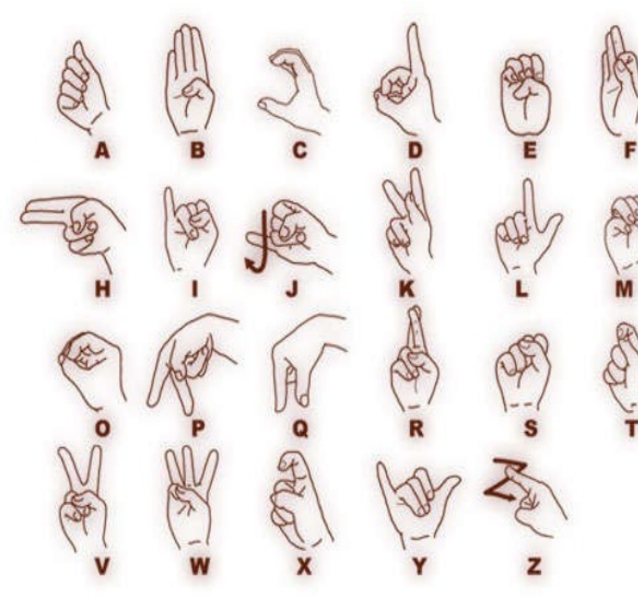
\includegraphics[scale=0.7]{gambar/SIBI Gesture.png}
  % Keterangan gambar yang diinputkan
  \caption{Gesture tangan untuk SIBI }
  % Label referensi dari gambar yang diinputkan
  \label{fig:Sibi}
\end{figure}
\subsection{Object Detection}
\emph{Object Detection} adalah teknik visi komputer yang membantu mengidentifikasi dan menemukan objek dalam gambar dan video. Dengan bentuk identifikasi dan pelokalan ini, deteksi objek dapat digunakan untuk menghitung jumlah item dalam sebuah skenario, menemukan dan mengidentifikasi mereka dengan tepat, serta memberikan nama. Pendeteksian objek tetap menjadi salah satu aspek paling mendasar dan menantang dalam aplikasi visi komputer dan pemahaman citra. Kemajuan signifikan dalam deteksi objek telah dicapai melalui representasi objek yang lebih baik dan penggunaan model jaringan saraf dalam (deep neural networks). Metode deteksi objek telah berkembang pesat dengan penggunaan jaringan saraf konvolusional (CNN) dan algoritme khusus seperti YOLO (You Only Look Once) dan SSD (Single Shot Multibox Detector).
Selain kerangka YOLO, kemajuan juga telah dicapai di bidang deteksi objek dan pemrosesan gambar.Memperluas beberapa metode terkenal lainnya. Teknologi seperti R-CNN (Konvolusi Berbasis Wilayah), (Neural Networks nasional) dan penerusnya Fast R-CNN dan Faster R-CNN.
Ini memainkan peran penting dalam meningkatkan akurasi deteksi objek. Metode ini bergantung pada dua proses Tahap tersebut melakukan pencarian selektif untuk menghasilkan proposal wilayah dan menghasilkan jaringan saraf konvolusional.Klasifikasi dan penyempurnaan area ini. Pendekatan penting lainnya adalah Single-Shot MultiBox Detector (SSD), yang mirip dengan YOLO dalam mengutamakan kecepatan dan efisiensi dengan menghilangkan kebutuhan akan langkah proposal wilayah secara terpisah. Di sisi lain, metode seperti Mask R-CNN telah meningkatkan kemampuan deteksi objek hingga mencakup segmentasi instans, memungkinkan pelokalan objek yang lebih presisi hingga tingkat piksel. Perkembangan ini, bersama metode lainnya seperti RetinaNet dan EfficientDet, secara kolektif telah memperkaya keragaman algoritma deteksi objek. Setiap algoritma ini menawarkan keseimbangan yang berbeda antara kecepatan, akurasi, dan tingkat kompleksitas, yang dirancang untuk memenuhi berbagai kebutuhan aplikasi dan batasan komputasi.
\subsection{YOLO(You Look Only Once)}
    YOLO (You Only Look Once) adalah salah satu algoritma deteksi objek dalam visi komputer yang dirancang untuk mendeteksi dan mengidentifikasi objek dalam gambar atau video secara cepat dan akurat. YOLO bekerja dengan cara menganalisis gambar secara keseluruhan dalam satu kali pemrosesan (hence "You Only Look Once"), berbeda dengan metode lainnya yang sering memproses gambar secara bertahap atau melalui beberapa langkah, seperti mengidentifikasi wilayah objek terlebih dahulu baru kemudian mengklasifikasikan objek tersebut.
Pada dasarnya, YOLO membagi gambar menjadi grid dan, untuk setiap grid, memprediksi berbagai kotak pembatas (bounding boxes) dan kemungkinan kelas objek yang ada di dalamnya. Hal ini memungkinkan YOLO untuk mendeteksi beberapa objek dalam satu gambar secara bersamaan dalam satu waktu pemrosesan, sehingga sangat efisien dalam hal kecepatan.
\subsection{YOLOv11}
YOLOv11 merupakan iterasi terbaru dalam seri pengembangan YOLO yang memperkenalkan peningkatan arsitektur baru, termasuk mekanisme perhatian yang lebih baik, lapisan ekstraksi fitur yang lebih dalam, dan paradigma deteksi tanpa jangkar (anchor-free). Inovasi-inovasi ini dirancang untuk mengatasi tantangan dalam mendeteksi kendaraan yang lebih kecil, tersembunyi, atau bergerak cepat, sambil mempertahankan kemampuan inferensi waktu nyata. YOLOv11 juga dioptimalkan untuk percepatan perangkat keras, membuatnya lebih kompatibel dengan perangkat tepi yang digunakan dalam aplikasi kritis seperti deteksi emosi dan sistem transportasi cerdas.
Peningkatan dalam YOLOv11, khususnya dengan pengenalan deteksi tanpa jangkar dan mekanisme perhatian yang lebih baik, menandakan langkah maju dalam pengembangan sistem deteksi kendaraan yang kuat dan dapat diskalakan.
Penggunaan YOLOv11 ini bertujuan untuk mengevaluasi kinerja YOLOv11 dalam konteks deteksi objek pada kursi roda, dengan fokus pada kemampuannya untuk menangani skenario deteksi yang kompleks dan waktu nyata. Hasil evaluasi YOLOv11 dibandingkan dengan pendahulunya, YOLOv8, menggunakan metrik utama seperti presisi, recall, dan mean average precision (mAP).
\begin{figure} [H] \centering
  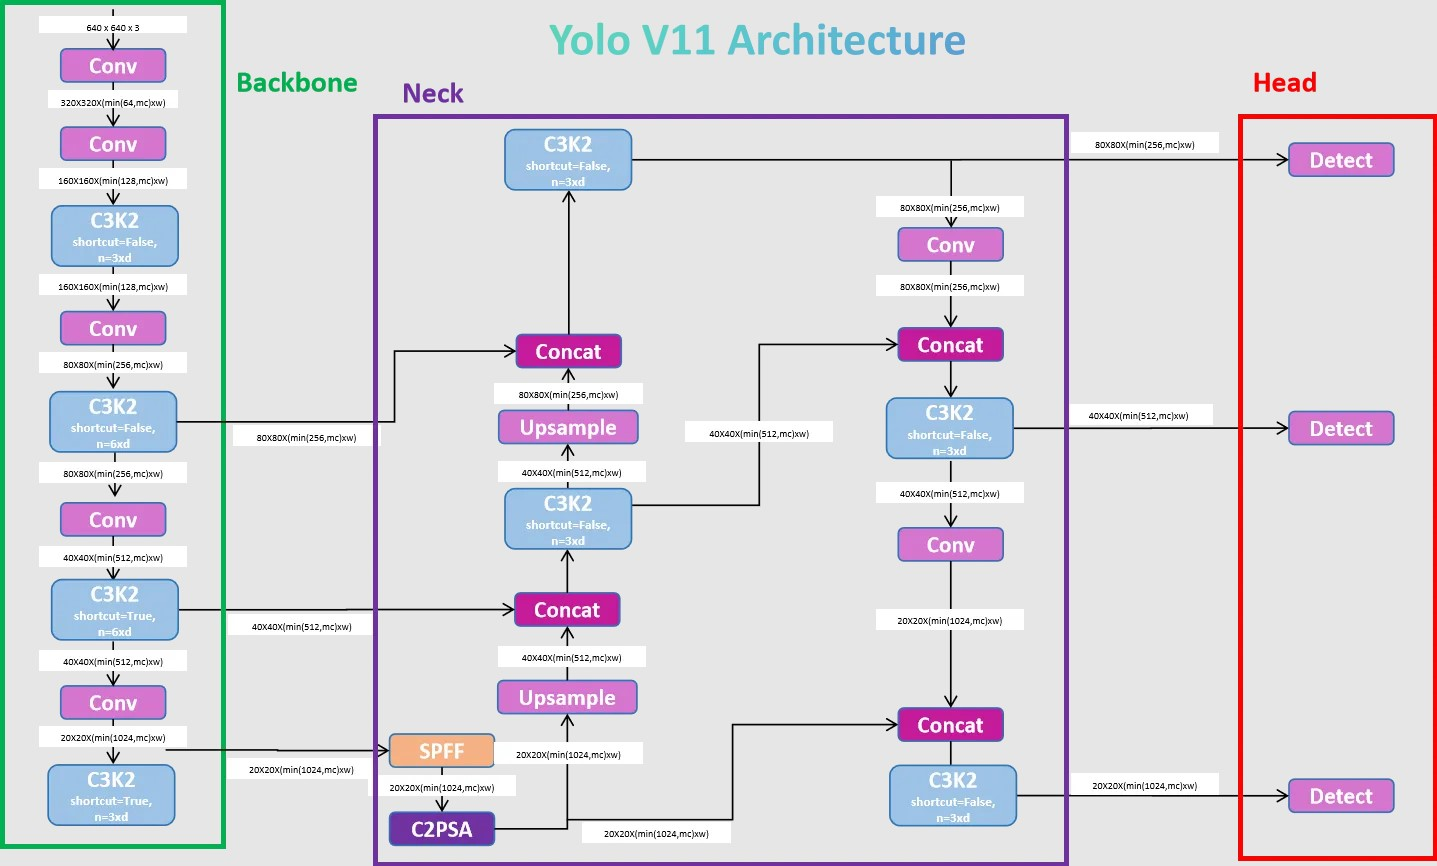
\includegraphics[width=\textwidth]{gambar/Arsitektur YOLOv11.jpg}
  \caption{Arsitektur dari YOLOv11 }
  \label{fig:YOLOv11}
\end{figure}
\subsection{LSTM(Long Short-Term Memory)}
\emph{Long Short-Term Memory} (LSTM) (LSTM) adalah bentuk RNN yang sering digunakan untuk menghindari masalah Penumpukan dengan gradasi, ketergantungan jangka panjang pada memproses atau membuat prediksi ke data deret waktu. RNN cenderung memiliki penumpukan pada gradien yang menyebabkan nilai gradien saling bertabrakan sehingga terdapat nilai gradien yang tidak jelas dan dapat menghilangkan nilai akumulasinya sehingga diperlukan LSTM untuk menghindari hal tersebut terjadi\cite{Cholissodin2019}.

Menurut Sepp Hochreiter dan Jurgen Schmidhuber, model LSTM terbentuk dari berbagai rangkaian sel memori yang dapat menggantikan sel neuron pada hidden layer dari RNN. Model LSTM dapat menyaring data atau informasi memlalu struktur gates untuk dapat mempertahankan informasi yang berhubungan dan mengubah keadaan dari sel memori. Struktur gerbang tersebut mencakup input gate, forgate gate, dan output gate\cite{Larasati2021}. 
\begin{figure} [H] \centering
  % Nama dari file gambar yang diinputkan
  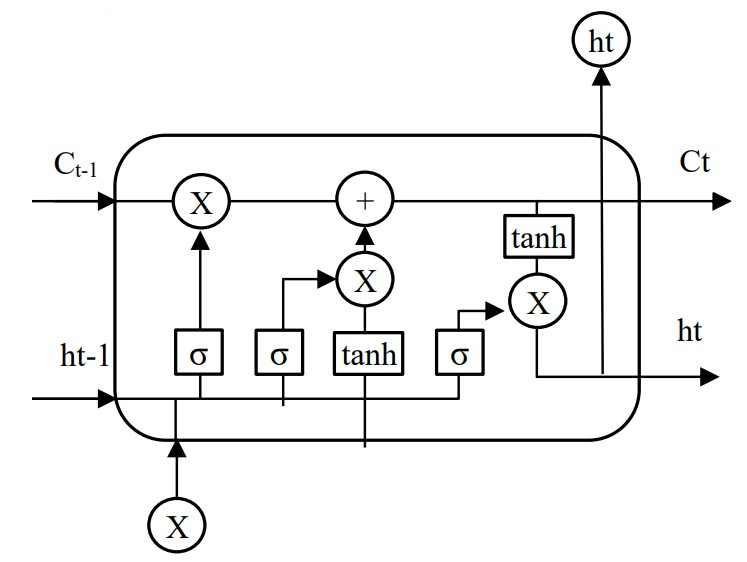
\includegraphics[scale=0.55]{gambar/LSTM.jpg}
  % Keterangan gambar yang diinputkan
  \caption{Arsitektur dari LSTM }
  % Label referensi dari gambar yang diinputkan
  \label{fig:Arsitektur LSTM }
\end{figure}
LSTM terdiri dari rangkaian sel memori yang unik dan model LSTM menyaring informasi
melalui struktur gerbang. Pada LSTM terdapat 3 gerbang atau Gates Unit dan 1 Cell states, yaitu input gates, forget gate, output gates, dan cell states. Persamaan dari setiap gate sebagai berikut:
\subsubsection{Input gates}
\emph{Input gate}menerima informasi berupa \emph{hidden state} yang berasal dari sel sebelumnya dan informasi baru yang berasal dari masukan saat ini, dan informasi tersebut digabungkan dan diproses menggunakan fungsi sigmoid dan tanh. Hasil dari fungsi sigmoid mengubah nilai dari 0 menjadi 1 dan menentukan informasi mana yang diperbarui. Nilai yang mendekati 0 berarti informasi tersebut tidak penting, dan nilai yang mendekati 1 berarti informasi tersebut penting. Hasil fungsi Tanh berupa nilai antara -1 dan 1 digunakan untuk membantu sel mempelajari informasi dengan lebih baik.
 Persamaan dari \emph{input gate} adalah sebagai berikut:
\begin{equation}
  \label{eq:InputGate}
  i_t = \sigma(W_i \times X_i + U_i \times h_{t-1} + b_i)
\end{equation}
Dalam persamaan ini, \( i_t \) mewakili nilai dari input gate, yang dihitung dengan menggunakan fungsi aktivasi sigmoid \( \sigma \), yang menghasilkan output antara 0 dan 1. Ini memungkinkan model untuk mengontrol secara dinamis seberapa banyak informasi dari input saat ini (\( X_i \)) dan keadaan tersembunyi sebelumnya (\( h_{t-1} \)) yang akan diterima dan disimpan dalam memori. Faktor \( W_i \) dan \( U_i \) adalah bobot yang masing-masing terkait dengan input \( X_i \) dan keadaan tersembunyi sebelumnya \( h_{t-1} \), sementara \( b_i \) adalah bias yang membantu menyesuaikan perhitungan tersebut.
\subsubsection{Forget gates}
\emph{Forget gates} memutuskan informasi apa yang akan disimpan atau dibuang. Forget gate menerima informasi berupa \emph{hidden state} yang berasal dari sel sebelumnya dan informasi baru yang berasal dari \emph{input} saat ini. Informasi ini kemudian digabungkan dan diproses menggunakan fungsi sigmoid sehingga menghasilkan hasil dalam bentuk 0 hingga  1. Semakin dekat hasil yang diperoleh ke 0, semakin banyak informasi yang dibuang, dan sebaliknya, semakin dekat hasil yang diperoleh ke 1, semakin banyak informasi yang disimpan. Persamaan dari \emph{forget gate} adalah sebagai berikut:
\begin{equation}
  \label{eq:ForgetGate}
  f_t = \sigma(W_f \times X_t + U_f \times h_{t-1} + b_f)
\end{equation}
Pada dasarnya, forget gate memeriksa data baru (\( X_t \)) dan informasi historis dari hidden state sebelumnya (\( h_{t-1} \)) untuk memutuskan seberapa besar kontribusi \( c_{t-1} \) yang akan diteruskan ke sel memori pada waktu \( t \). Ini adalah langkah penting dalam mengontrol ``memori jangka panjang'' pada LSTM, yang memungkinkan jaringan untuk menangani dependensi jangka panjang dalam data.

Jika nilai \( f_t \) mendekati 0, maka sebagian besar informasi dari memori sebelumnya akan dilupakan. Sebaliknya, jika \( f_t \) mendekati 1, informasi tersebut akan dipertahankan dalam memori selanjutnya. Ini membantu LSTM mengelola informasi yang relevan dan membuang informasi yang tidak berguna.
\subsubsection{Output gates}
\emph{Output gates} menentukan \emph{hidden state} yang dikirim ke sel berikutnya.\emph{Output gate} menerima informasi berupa \emph{hidden state} yang berasal dari sel sebelumnya, informasi baru yang berasal dari masukan saat ini, dan informasi tersebut digabungkan dan diproses dengan fungsi sigmoid. Status sel baru ditangani melalui fungsi tanh. Hasil fungsi Tanh dikalikan dengan hasil fungsi sigmoid untuk memperoleh informasi yang disimpan dalam keadaan tersembunyi baru. Status tersembunyi dan status sel baru ditransfer ke sel berikutnya. Berikut adalah persamaan dari \emph{output gate}:
\begin{equation}
  \label{eq:OutputGate}
  o_t = \sigma(W_o \times X_i + U_o \times h_{t-1} + b_o)
\end{equation}
Output gate pada LSTM mengontrol informasi yang akan diteruskan dari cell state \( c_t \) ke hidden state \( h_t \) dan akhirnya menjadi output model. Ini penting karena hidden state (\( h_t \)) membawa informasi yang diperlukan untuk prediksi pada langkah berikutnya, dan juga dapat digunakan sebagai output model dalam tugas-tugas seperti klasifikasi atau prediksi deret waktu.

Setelah output gate dihitung, informasi dari cell state \( c_t \) diubah dengan fungsi tanh (fungsi aktivasi hiperbolik tangen) untuk memastikan nilai berada dalam rentang yang sesuai sebelum diteruskan melalui output gate. Prosesnya adalah sebagai berikut:
\begin{equation}
  \label{eq:OutputGate dari LSTM}
  h_t = o_t \times \tanh(c_t)
\end{equation}
Di sini, \( \tanh(c_t) \) mengubah nilai cell state menjadi nilai yang lebih terkontrol sebelum dihasilkan sebagai output.
\subsection{Mediapipe}
MediaPipe adalah kerangka kerja yang dirancang oleh Google untuk dikembangkan.
Saluran pengenalan waktu nyata. MediaPipe memungkinkan pengembang untuk berintegrasi
Integrasikan berbagai jenis data sensor seperti video, audio, dan data lainnya ke dalam satu platform ini efisien dan dapat berjalan di berbagai perangkat mulai dari seluler hingga desktop.
Framework ini menggunakan konsep “grafik”, jadi setiap node dalam grafik Ini adalah "kalkulator" yang melakukan tugas-tugas tertentu seperti deteksi objek, pelacakan, dll. pose, atau segmentasi gambar. Masing-masing node ini dapat dikonfigurasi melalui GraphConfig.Salah satu penerapan MediaPipe yang paling dikenal adalah pada estimasi pose manusia menggunakan MediaPipe Pose. Metode ini menggabungkan estimasi pose 2D dengan model
humanoid yang lebih kompleks serta metode optimasi untuk mengestimasi sudut sendi pada
pose 3D. Metode ini terbukti efektif dalam mengatasi masalah ambiguitas kedalaman pada es-
timasi pose 3D dan dapat berjalan secara real-time bahkan pada perangkat tanpa GPU\cite{Lugaresi2019}.
\subsubsection{MediaPipe Pose}
MediaPipe Pose (MPP) adalah kerangka kerja sumber terbuka yang disediakan oleh Google.
Digunakan untuk mendapatkan perkiraan koordinat sendi manusia 2D dalam setiap bingkai gambar batang. MediaPipe Pose membangun saluran untuk memproses data kognitif dalam beberapa bagian untuk video menggunakan \emph{Machine Learning} (ML). Penerapan MPP
BlazePose mengekstrak 33 landmark 2D tubuh manusia seperti yang ditunjukkan.
Dapat dilihat pada Gambar 2.4. BlazePose adalah arsitektur pembelajaran mesin ringan yang memungkinkan kesamaan pekerjaan real-time di ponsel dan PC dengan inferensi CPU.Ketika menggunakan koordinat yang dinormalisasi untuk estimasi pose, rasio invers harus dikalikan dengan nilai piksel sumbu-y\cite{kim2023human}.
\begin{figure} [H] \centering
  % Nama dari file gambar yang diinputkan
  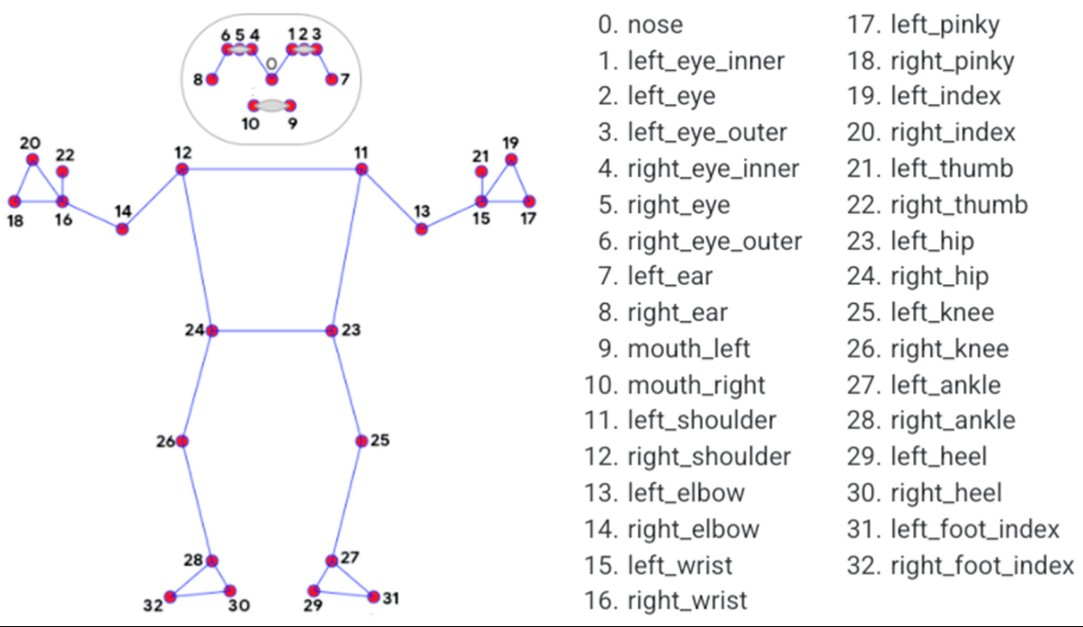
\includegraphics[scale=0.3]{gambar/mediapipepose.jpg}
  % Keterangan gambar yang diinputkan
  \caption{Pose MediaPipe }
  % Label referensi dari gambar yang diinputkan
  \label{fig:Pose MediaPipe }
\end{figure}

\subsection{Classification Performance}
\emph{Classification Performance} adalah sekumpulan metrik yang digunakan untuk mengevaluasi kinerja model klasifikasi. Metrik ini digunakan untuk menilai akurasi model, presisi, perolehan kembali, dan aspek lainnya. Ini sering digunakan untuk membandingkan model yang berbeda atau menyetel satu model untuk kinerja optimal. Metrik klasifikasi dapat dikelompokkan menjadi tiga kategori utama: Akurasi, sensitivitas, spesifisitas. Akurasi mengukur performa model secara keseluruhan dan biasanya merupakan metrik yang paling penting. Sensitivitas dan spesifisitas mengukur seberapa baik suatu model dapat membedakan kelas yang berbeda. Terakhir, metrik lain seperti skor AUC, skor F1, dan skor Kappa mengukur akurasi dan pengenalan model.  Dalam hal ini, confusion matrix merupakan salah satu perhitungan yang sering digunakan dalam kasus
pengklasifikasian.
\subsubsection{Confusion Matrix}
\emph{Confusion matrix} adalah salah satu pengukuran paling sederhana
Mencari tingkat nilai kebenaran dan keakuratan model. \emph{Confusion matrix}
merupakan tabel dua dimensi berisi data aktual dan prediksi, masing-masing dengan kelasnya. Data aktual ada di bagian kolom tabel dan data prediksi ada di bagian baris tabel. Gambar 2.5 merupakan representasi visual dari perhitungan confusion matrix. 
\begin{figure} [H] \centering
  % Nama dari file gambar yang diinputkan
  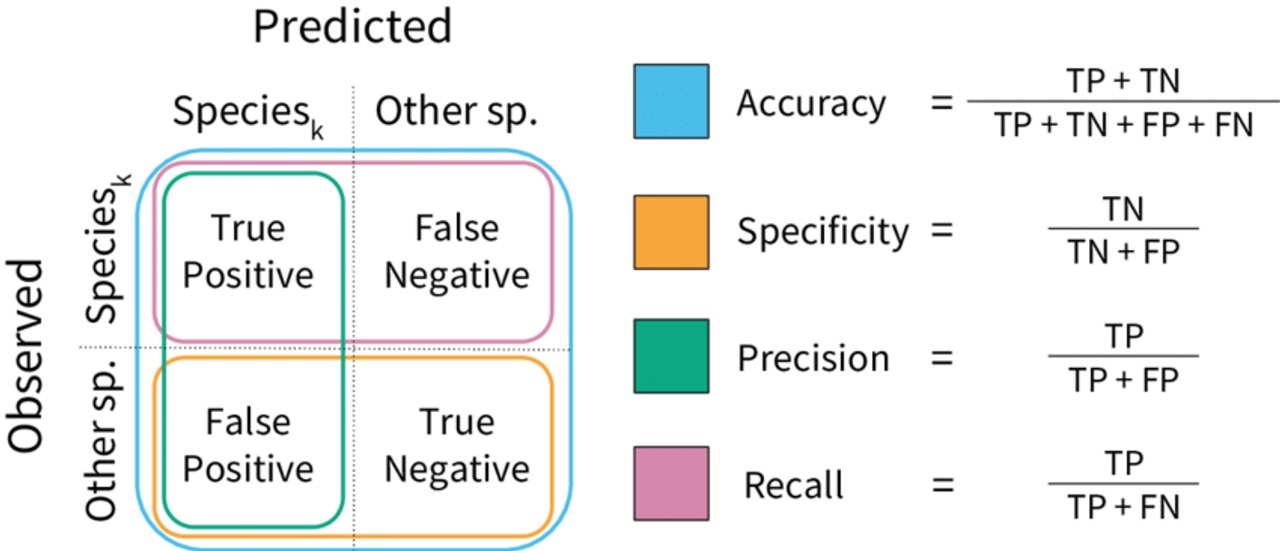
\includegraphics[scale=0.3]{gambar/confusionmatrix.jpg}
  % Keterangan gambar yang diinputkan
  \caption{Confusion Matrix }
  % Label referensi dari gambar yang diinputkan
  \label{fig:Confusion matrix }
\end{figure}

\subsection{Evaluation Matrix}
\emph{Evaluation Matrix} adalah cara untuk mengevaluasi sejumlah besar peringkat secara objektif. Pilihan untuk beberapa kriteria. Kriteria ini akan diprioritaskan sebelum evaluasi. Ini telah dibuat dengan lebih menekankan pada item yang paling penting.Terdapat dua tingkatan dalam \emph{evaluation matrix}. tingkat pertama ini bertindak sebagai filter di mana setiap opsi dievaluasi berdasarkan kriteria yang diperlukan pilihan-pilihan itu
yang memenuhi semua kriteria yang dipersyaratkan akan maju ke tingkat kedua dan dievaluasi kriteria prioritas. 

Metrik seperti akurasi, presisi, recall adalah kunci saat mengevaluasi seberapa efektif suatu model dalam mendeteksi dan mengidentifikasi objek. 
Lebih lanjut, analisis akurasi memberikan wawasan kuantitatif yang signifikan mengenai
kinerja algoritma deteksi objek, memberikan detail lebih lanjut mengenai kemampuan algo-
ritma dalam menghasilkan deteksi yang akurat. Mengenali kesalahan melalui metrik evaluasi
adalah langkah kritis dalam penelitian deteksi, seperti dalam kasus deteksi asap yang kami
teliti. Langkah ini memfasilitasi identifikasi dan pemahaman tentang potensi kesalahan dalamalgoritma, yang dapat membuka jalan untuk perbaikan dan peningkatan metode deteksi. Selanjutnya, metrik evaluasi juga mendukung pengoptimalan hiperparameter algoritma.
Dalam konteks penelitian ini, berbagai indikator evaluasi telah diterapkan, termasuk presisi, recall, dan Mean Average Precision (mAP). . Dengan menggabungkan metode evaluasi ini,Penelitian ini bertujuan untuk menyajikan analisis komprehensif terhadap kinerja algoritma deteksi objek yang sedang ditinjau.

\subsection{Intersection over Union(IoU)}
Intersection over Union adalah metrik populer untuk mengukur akurasi pelokalan dan menghitung kesalahan pelokalan dalam model deteksi objek. Ini menghitung jumlah tumpang tindih antara dua kotak pembatas—kotak pembatas yang diprediksi dan kotak pembatas kebenaran dasar. IoU adalah rasio perpotongan luas dua kotak dengan luas gabungannya. Kotak pembatas kebenaran dasar dan kotak pembatas yang diantisipasi keduanya mencakup area gabungan, yang merupakan penyebutnya.
\begin{figure} [H] \centering
  % Nama dari file gambar yang diinputkan
  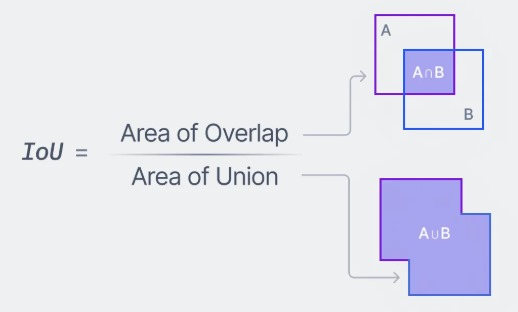
\includegraphics[scale=0.6]{gambar/IoU.jpg}
  % Keterangan gambar yang diinputkan
  \caption{Penggambaran dari IoU }
  % Label referensi dari gambar yang diinputkan
  \label{fig:Intersection over Union }
\end{figure}
IoU, atau Intersection over Union, merupakan metode penilaian yang mengukur efektivi-
tas model deteksi objek dengan membandingkan area overlap antara prediksi model dan posisi
objek aktual. Skala nilai IoU berada antara 0 hingga 1, nilai yang lebih dekat ke 1 menandakan prediksi yang sangat akurat terhadap objek sebenarnya. Nilai IoU yang lebih tinggi menunjukkan bahwa model tersebut lebih tepat dalam mengidentifikasi dan menentukan lokasi objek. Dalam skenario penelitian, misalnya pengenalan otomatis seekor hewan dalam sebuah gambar, model pembelajaran mendalam akan menciptakan sebuah kotak pembatas sebagai
prediksi lokasi hewan tersebut. Kotak pembatas ini lalu dibandingkan dengan kotak kebenaran
dasar—area yang telah ditentukan secara manual sebagai lokasi sebenarnya dari hewan dalam
gambar. IoU kemudian dihitung untuk menilai seberapa baik kotak prediksi menutupi kotak
kebenaran dasar, dengan mempertimbangkan area bersama dan area gabungan dari kedua kotak
tersebut.
\begin{figure} [H] \centering
  % Nama dari file gambar yang diinputkan
  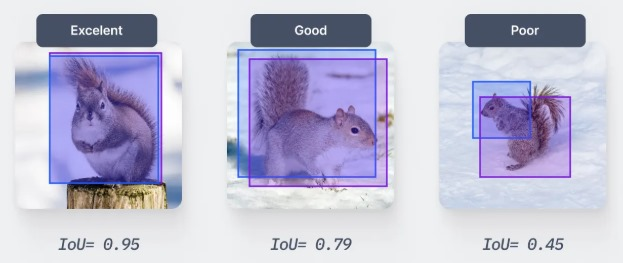
\includegraphics[scale=0.6]{gambar/bounding boc.jpg}
  % Keterangan gambar yang diinputkan
  \caption{Contoh perbandingan performa IoU }
  % Label referensi dari gambar yang diinputkan
  \label{fig:Perbandingan Intersection over Union }
\end{figure}
IoU menawarkan metode kuantitatif untuk mengevaluasi seberapa akurat model dalam
mengenali dan menandai objek dalam gambar. Dalam proses pelatihan, nilai IoU minimal yang
ditetapkan memungkinkan penetapan batas bagi kotak prediksi untuk dianggap cocok dengan
deteksi yang benar, memfasilitasi penyesuaian antara tingkat akurasi deteksi dan insiden false positif. Penentuan batas IoU tidak bersifat tetap dan dapat disesuaikan, dengan 0,5 yang menjadi standar patokan awal. Kotak prediksi dengan IoU minimal 0,5 terhadap deteksi positif dianggap valid. Penyesuaian ambang nilai ini mempengaruhi balance antara presisi dan daya tangkap, dengan peningkatan nilai ambang cenderung mengurangi kesalahan positif namun berpotensi mengabaikan beberapa deteksi valid.Penggunaan nilai kebenaran dasar dalam IoU merupakan perbandingan standar antara prediksi dan kondisi aktual objek yang diidentifikasi. Penandaan kotak kebenaran dasar, dilakukan secara manual oleh pakar, menentukan batas pasti objek dalam gambar. Skor IoU yang dihasilkan dari perbandingan antara prediksi model dengan batas ini memberikan wawasan terhadap efektivitas model dalam deteksi objek. Dataset kebenaran dasar, yang meliputi kotak pembatas yang ditandai secara manual, menjadi kunci dalam proses evaluasi ini, memberikan dasar objektif untuk mengukur kinerja algoritme deteksi objek\cite{Shah2023}.

\subsection{Tensorflow}
TensorFlow adalah sistem pembelajaran mesin yang beroperasi dalam skala besar dan di lingkungan yang heterogen. TensorFlow menggunakan grafik aliran data untuk merepresentasikan komputasi, status bersama, dan operasi yang mengubah status tersebut. Ini memetakan node grafik aliran data di banyak mesin dalam sebuah cluster, dan di dalam mesin di beberapa perangkat komputasi, termasuk CPU multicore, general-purpose GPU, dan ASIC yang dirancang khusus yang dikenal sebagai Tensor Processing Units (TPU). Arsitektur ini memberikan fleksibilitas kepada pengembang aplikasi. TensorFlow memungkinkan pengembang bereksperimen dengan pengoptimalan baru dan algoritma pelatihan. TensorFlow mendukung berbagai aplikasi, dengan dukungan yang sangat kuat untuk pelatihan dan inferensi pada jaringan neural dalam. Beberapa layanan Google menggunakan TensorFlow dalam produksinya, dan telah banyak digunakan untuk penelitian pembelajaran mesin.\
\subsubsection{Tensorflow-Keras}
Keras merupakan library yang dikembangkan oleh Francois Chollet. Keras ini dirancang oleh pengembang agar cepat, mudah diimplementasikan, dan modular secara alami. Keras diadopsi sebagai API tingkat tinggi untuk mengembangkan algoritma pembelajaran mendalam alias deep learning. 

\subsection{ESP-32}
ESP32 adalah modul mikrokontroler terintegrasi yang memiliki fitur lengkap dan kinerja tinggi. Modul ini merupakan pengembangan dari ESP8266, yang merupakan modul WiFi populer. ESP32 memiliki dua prosesor komputasi, satu prosesor untuk mengelola jaringan WiFi dan Bluetooth, serta satu prosesor lainnya untuk menjalankan aplikasi. Dilengkapi dengan memori RAM yang cukup besar untuk menyimpan data. Fitur yang berguna seperti TCP/IP, HTTP, dan FTP. Modul ini juga dilengkapi fitur pemrosesan sinyal analog, dukungan untuk sensor, dan dukungan untuk perangkat masukan/keluaran (I/O) digital. ESP32 juga memiliki dukungan untuk konektivitas Bluetooth. Dapat digunakan untuk mengendalikan perangkat yang terhubung dengan Bluetooth.
\cleardoublepage
\chapter{METODOLOGI}
Penelitian ini dilakukan sesuai dengan desain sistem berikut beserta implementasinya. Desain sistem adalah konsep dari pembuatan dan perancangan infrastruktur dan kemudian diwujudkan dalam bentuk alur yang harus dikerjakan
% Ubah konten-konten berikut sesuai dengan isi dari metodologi

\section{Metode Penelitian}
Metode penelitian yang akan digunakan pada penelitian ini adalah penelitian pengembangan dari Richey dan Klein\cite{Sugiyono2019}. Metode ini memiliki tiga tahapan yaitu \emph{planning}, \emph{production}, dan \emph{evaluation}. Berikut adalah diagram dari metode yang akan digunakan dalam penelitian ini.
\begin{figure} [H] \centering
  % Nama dari file gambar yang diinputkan
  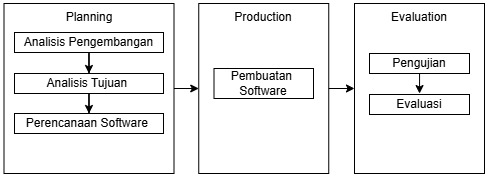
\includegraphics[scale=0.6]{gambar/metodologi penelitian.jpg}
  % Keterangan gambar yang diinputkan
  \caption{Diagram alur penelitian}
  % Label referensi dari gambar yang diinputkan
  \label{fig:Metode penelitian }
\end{figure}
\subsection{Perencanaan(Planning)}
Pada bagian perencanaan, peneliti melakukan analisis pengembangan terhadpat kursi roda yang sudah ada sebelumnya. Analisis pengembangan ini diperlukan agar penilit dapat mengetahui hal apa yang bisa dikembang dari kursi roda. Berdasarkan hasil dari analisis pengembangan, hal yang dapat dikembangkan dari kursi roda adalah bagian \emph{software}.
\subsection{Produksi(Production)}
Tahan produksi meliputi pembuatan dari \emph{software} dari kursi roda berdasarkan dari perencanaan software dan analisis tujuan yang telah ditentukan di tahan \emph{planning}.
\subsection{Evaluasi(Evaluation)}
Pada tahap ini, dilakukan pengujian secara bertahap untuk memastikan kursi roda dapat beroperasi sesuai dengan tujuan yang telah ditetapkan.

\section{Analisis sistem}
Sebelum memulai pengembangan sistem, penting untuk melakukan analisis terhadap sistem.
Analisis ini diperlukan untuk mengetahui kebutuhan dan tujuan yang ingin dicapai. Tujuan dari analisis kebutuhan adalah identifikasi berbagai elemen yang diperlukan untuk sistem, baik dari sudut pandang fungsional maupun non-fungsional. Untuk memastikan bahwa sistem yang dikembangkan memenuhi persyaratan perlu ditetapkan spesifikasi dan persyaratan.

\subsection{Analisis Kebutuhan}
Analisis kebutuhan dilakukan dengan mengumpulkan data dari studi literatur terkait. Analisis ini bertujuan untuk mengidentifikasi fitur-fitur dan spesifikasi teknis yang diperlukan dalam pengembangan sistem. Berdasarkan hasil analisis, beberapa
kebutuhan sistem yang harus dipenuhi adalah sebagai berikut:
\begin{enumerate}
    \item Penggunaan gesture SIBI sebagai metode utama kendali kursi roda cerdas.
    \item Penelitian pada penggunaan LSTM untuk pengenalan dan deteksi gesture tangan SIBI yang dikombinasikan dengan perangkat keras seperti kamera.
    \item Penggunaan LSTM pada pemrosesan urutan data gesture yang diambil dari kamera.
    \item Pengembangan smart braking system untuk meningkatkan keselamatan pengguna kursi roda dalam mendeteksi objek di sekitar kursi roda dan melakukan pengereman otomatis. 
    \item Sistem smart breaking ini akan berfungsi untuk mendeteksi manusia dan objek lain di lingkungan sekitarnya.
    \item Penelitian difokuskan pada pengembangan dan integrasi antara perangkat keras (kamera, motor kursi roda) dan perangkat lunak kontrol kursi roda dan smart braking system.
    \item Pengontrol kursi roda akan diimplementasikan untuk memberikan respon sesuai dengan gestur yang dipanggil dan berhenti otomatis ketika mendeteksi manusia di depannya.
\end{enumerate}
\subsection{Analisis Tujuan}
Berdasarkan hasil analisis kebutuhan, tujuan pengembangan dari sistem ini ditetapkan untuk
memastikan bahwa sistem yang dikembangkan dapat memenuhi spesifikasi dan operasional
yang diperlukan. Adapun tujuan dari ingin dicapai dalam pengembangan sistem ini adalah:
\begin{enumerate}
    \item Membuat sebuah sistem untuk mendeteksi gestur SIBI menggunakan LSTM.
    \item Membuat sebuah sistem untuk mendeteksi objek menggunakan YOLOv11 untuk sistem pengereman otomatis.
\end{enumerate}

\section{Rancangan Penelitian}
\begin{figure} [H] \centering
  % Nama dari file gambar yang diinputkan
  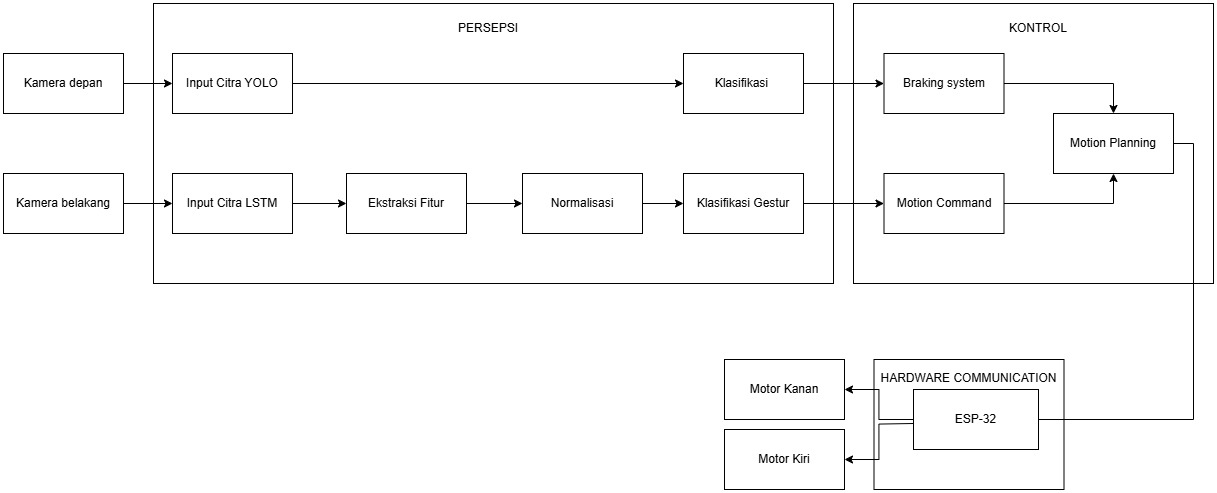
\includegraphics[scale=0.4]{gambar/rancangan penelitian.jpg}
  % Keterangan gambar yang diinputkan
  \caption{Blok diagram dari sistem}
  % Label referensi dari gambar yang diinputkan
  \label{fig:rancangan penelitian}
\end{figure}
Pada tahap ini, sistem akan diterapkan sesuai dengan desain dan implementasi yang telah direncanakan sebelumnya. Diagram ini mencakup dari pengembangan software, alur sistem, dan implementasi infrastruktur. 
\section{Software}
\begin{figure} [H] \centering
  % Nama dari file gambar yang diinputkan
  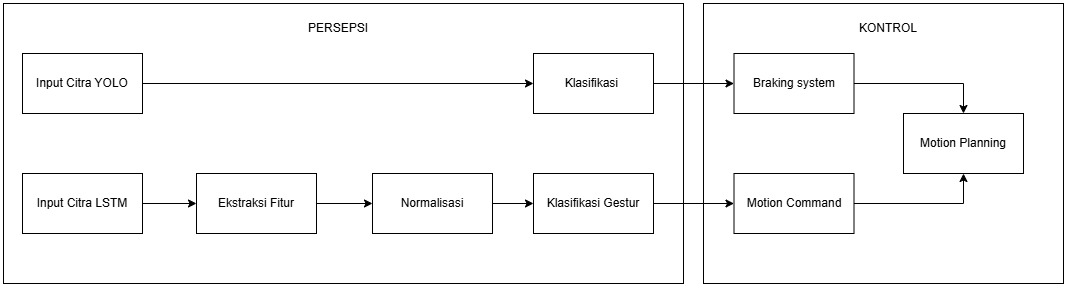
\includegraphics[scale=0.4]{gambar/software new.jpg}
  % Keterangan gambar yang diinputkan
  \caption{Diagram dari \emph{software}}
  % Label referensi dari gambar yang diinputkan
  \label{fig:diagram software}
\end{figure}
Pada tahap ini, merupakan pembuatan dari software yang telah ditentukan pada perencanaan \emph{software}. Gambar 3.2 merupakan blok diagram dari alur yang akan dijelaskan sebagai berikut:

\subsection{Input Citra YOLO}
Input untuk YOLO biasanya berupa citra dalam format digital (misalnya JPG atau PNG) yang telah diubah ukurannya sesuai dengan kebutuhan model. Sebelum dimasukkan ke model, citra tersebut dinormalisasi, yaitu nilai pikselnya diubah menjadi rentang 0 hingga 1 untuk mempercepat proses komputasi. YOLO membagi citra menjadi grid, di mana setiap grid bertanggung jawab untuk memprediksi bounding box, confidence score, dan kelas objek di dalam grid tersebut. Proses ini menghasilkan output berupa koordinat bounding box, skor probabilitas, dan label kelas untuk setiap objek yang terdeteksi.

\subsection{Labelling menggunakan Roboflow}
Input citra yang didaptkan tadi lalu akan dilabeli dan diaugmentasi. Dimana Roboflow digunakan untuk melakukan proses labeli dan augmentasi ini. Roboflow memiliki tools yang mumpuni dalam melakukan labeling. Dimana terdapat beberapa proses yang akan dilakukan yaitu, import dataset, pelabelan dataset dan augmentasi dataset.

\begin{figure} [H] \centering
  % Nama dari file gambar yang diinputkan
  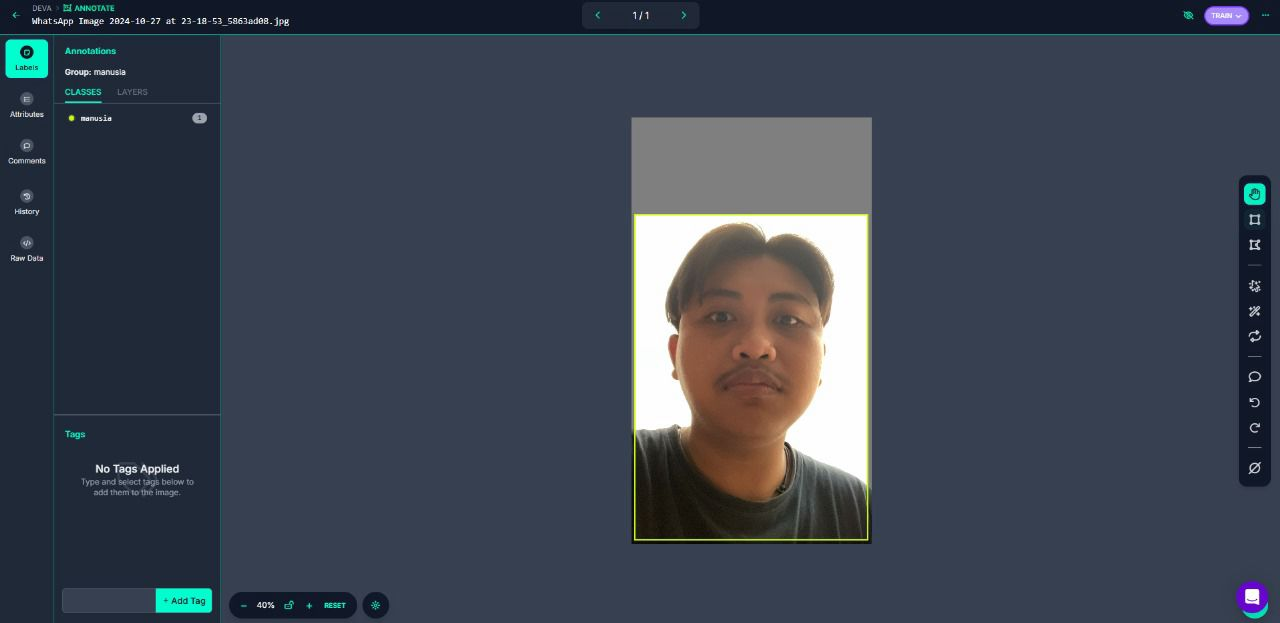
\includegraphics[scale=0.2]{gambar/devafoto.jpeg}
  % Keterangan gambar yang diinputkan
  \caption{Labeling pada Roboflow}
  % Label referensi dari gambar yang diinputkan
  \label{fig:rancangan penelitian}
\end{figure}

Dalam Proses anotasi penamaan class yang digunakan haruslah sesuai dengan objek yang akan dideteksi. Dalam Konteksi tugas akhir kali ini objek yang akan dideteksi adalah manusia. Maka digunakanlah nama manusia sebagai penamaan dari kelas yang akan digunakan. Adapun dalam proses anotasi harus diperhatikan objek yang akan dianotasikan harus sesuai agar tidak ada kesalahan model dalam mendeteksi. %Setelah selesai maka dataset akan terlihat seperti gambar dibawah. 

setelah seluruh gambar yang dipilih telah dianotasi. Maka disimpan dalam bentuk versi yang mudah diingat, apabila terjadi perubahan pada dataset maka akan disimpan dalam versi lain.

%Adapun fitur pemberian augmentasi pada dataset yang merupakan tools dari roboflow yang berguna untuk memberikan variasi dari dataset, gambar berikut adalah contoh pemberian augmentasi dataset. Setelah selesai pemberian augmentasi maka dataset ini sudah dapat digunakan untuk dilakukan klasifikasi menggunakan YOLOV8, YOLOV11 dan YOLOV12.

\subsection{Klasifikasi}
Klasifikasi dalam YOLO (You Only Look Once) adalah proses di mana model menentukan kategori atau kelas dari objek yang terdeteksi dalam sebuah citra. Setelah model YOLO mendeteksi keberadaan objek melalui bounding box, langkah berikutnya adalah mengklasifikasikan objek tersebut ke dalam salah satu kelas yang telah dilatih, seperti mobil, orang, hewan, atau benda lainnya, dalam penelitian kelas yang digunakan adalah manusia.

%Proses ini melibatkan softmax function atau sigmoid activation (tergantung pada versi YOLO) untuk menghasilkan probabilitas dari setiap kelas. Probabilitas ini menunjukkan keyakinan model bahwa objek dalam bounding box tersebut termasuk ke dalam kelas tertentu. Kelas dengan probabilitas tertinggi dipilih sebagai hasil klasifikasi. Kombinasi antara deteksi (bounding box) dan klasifikasi memungkinkan YOLO untuk mengenali posisi serta jenis objek dalam sebuah citra secara simultan.

\subsection{Klasifikasi YOLOV8}
Klasifikasi dilakukan setelah melakukan proses labelling yang akan dikenali menggunakan YOLOV8 yang telah ditraining untuk mengenali manusia yang terdapat pada citra. Model akan memberikan output berupa kelas yaitu manusia, nantinya hasil dari klasifikasi akan dijadikan acuan untuk melakukan \emph{braking}.

Model yang digunakan memiliki output kelas berupa manusia, adapun hasilnya berupa \emph{bounding box} pada manusia yang terdeteksi. Adapun arsitektur yang digunakan pada YOLOV8 

\begin{figure} [H] \centering
  % Nama dari file gambar yang diinputkan
  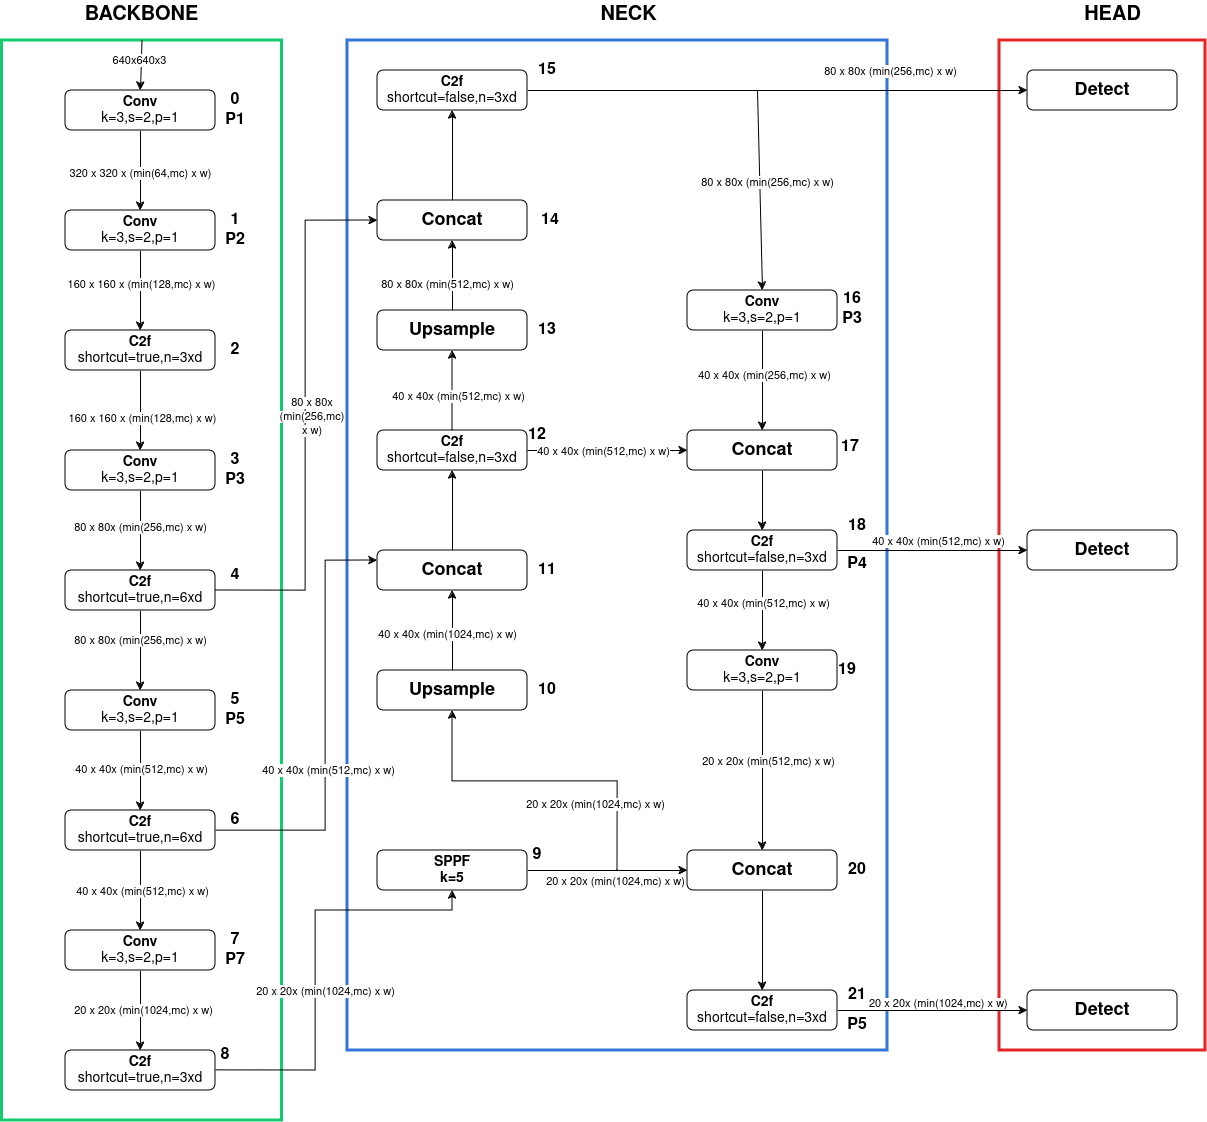
\includegraphics[scale=0.3]{gambar/yolov8.png}
  % Keterangan gambar yang diinputkan
  \caption{Blok diagram dari sistem}
  % Label referensi dari gambar yang diinputkan
  \label{fig:rancangan penelitian}
\end{figure}

Arsitektur YOLOV8 menggunakan \emph{convolutional neural network (CNN)} sebagai dasar dalam YOLO, jaringan CNN digunakan untuk ekstraksi fitur dari gambar yang telah diinputkan dan kemudian menerapkan jaringan lain untuk memprediksi bounding box dan kelas objek langsung dari gambar tersebut. Adapun selain lapisan CNN terdapat juga lapisan Concat, lapisan Upsampling, Blok SPPF, Blok C2f.

Adapun dalam arsitektur YOLOV8 dibagi menjadi bagian backbone, neck dan head. agar dapat memahami arsitektur YOLOV8 akan dibahas satu per satu fungsi dari lapisan dan blok yang digunakan pada YOLOV8. Lapisan Convolution (Conv) fungsinya yaitu melakukan operasi convolusi pada gambar input untuk mengekstraksi fitur pada gambar. operasi ini melibatkan filter pada gambar, mengkalikan dan menjumlahkan nilai nilai piksel untuk menghasilkan fitur map baru.

Blok C2f atau yang sering disebut dengan Cross Stage Spatial Network, dimana pada blok ini digabungka beberapa lapisan convolusi dengan skip connection, yang meningkatkan pemahaman konteks spasial dan fitur kompleks

Blok SPPF (spatial pyramid pooling fast) bertujuan untuk menangkap dari bebagai skala fitur map dengan menerapkan pooling pada beberapa tingkat. Sebagai contoh 1x1, 3x3 dan 5x5.

Lapisan Upsampling meningkatkan resolusi fitur map dengan memperbesar dimensinya menggunakan metode seperti neaarest neighbor atau bilinear interpolation, memungkinkan deteksi objek dengan resolusi yang lebih tinggi

Lapisan Concat (concatenate) menggabungkan dua atau lebih fitur map dari jalur berbeda dalam model. ini dilakukan dengan menggabungkan fitur map di sepanjang dimensi channel, sehingga mempertahankan  informasi dari berbagai tahap pemrosesan sebelumnya sehingga menghasilkan konteks yang lebih kaya untuk deteksi objek.

\subsection{Klasifikasi YOLOV11}
Klasifikasi pada YOLOV11 juga menggunakan data yang sudah dilabeling pada proses sebelumnya. Dimana output yang diharapkan dari training yaitu berupa kelas yaitu manusia.

YOLOV11 menggunakan arsitektur yang kurang lebih sama dengan YOLOV8 dengan perubahan pada Blok C2f yang diganti dengan Blok C3K2 yang merupakan upgrade untuk menghasilkan deteksi yang lebih baik dan lebih effisien. adapun arsitektur YOLOV11 sebagai 

\begin{figure} [H] \centering
  % Nama dari file gambar yang diinputkan
  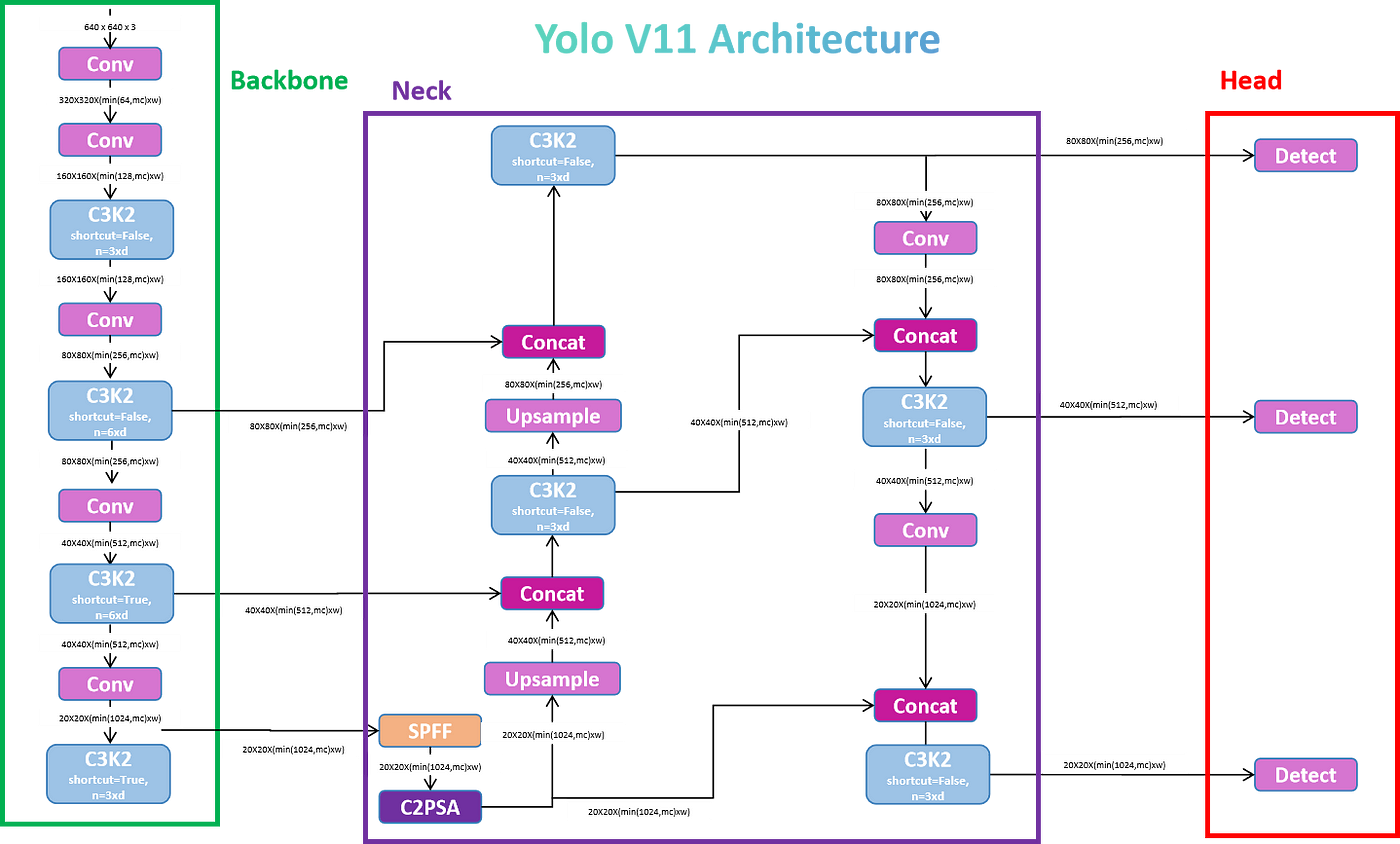
\includegraphics[scale=0.25]{gambar/yolov11.png}
  % Keterangan gambar yang diinputkan
  \caption{Blok diagram dari sistem}
  % Label referensi dari gambar yang diinputkan
  \label{fig:rancangan penelitian}
\end{figure}

Blok C3k2 berisi lapisan convolusi yang digabungkan dengan blok C3K dan lapisan concat. adapun lapisan ini digunakan untuk menghasilkan ekstraksi fitur yang lebih baik, terutama untuk objek yang berukuran kecil. Berikut merupakan isi dari Blok C2f pada YOLOV8 dan C3K2 pada YOLOV11.

\begin{figure} [H] \centering
  % Nama dari file gambar yang diinputkan
  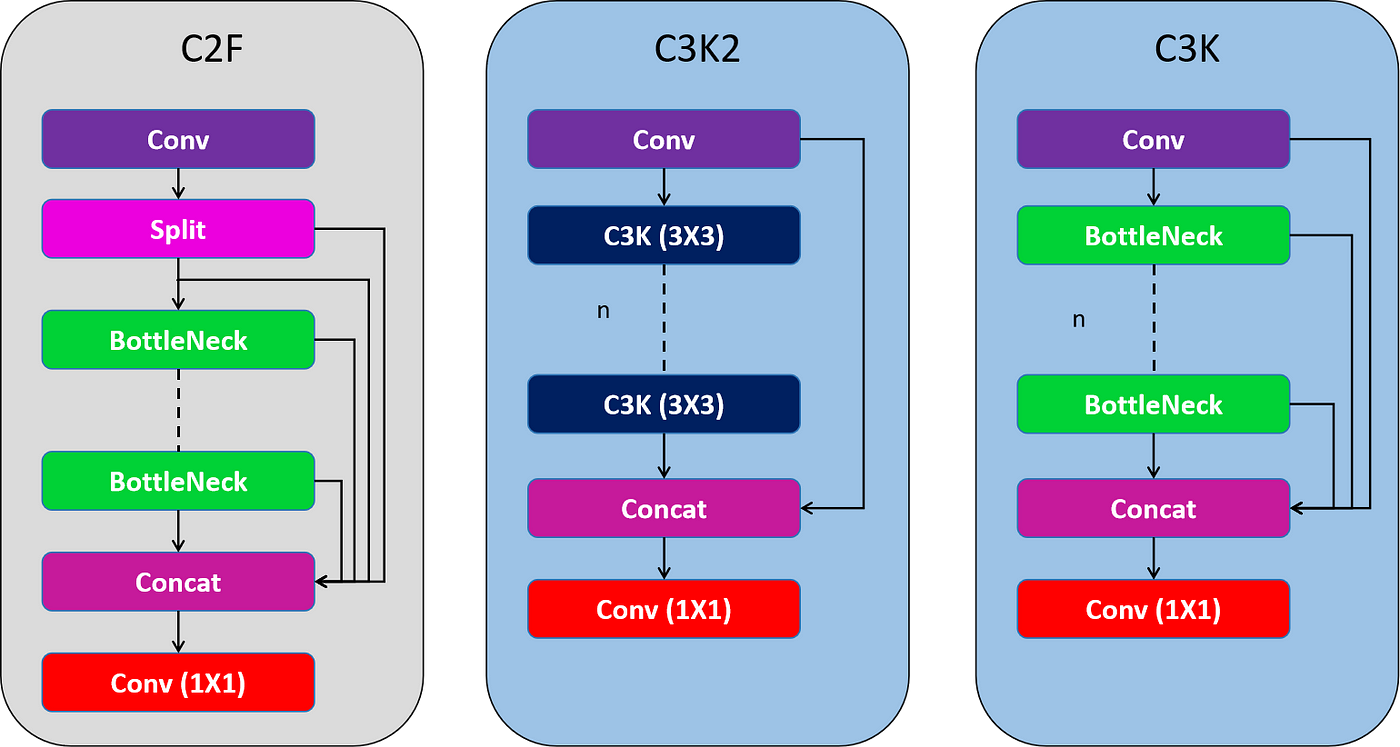
\includegraphics[scale=0.18]{gambar/c2f c3k2.png}
  % Keterangan gambar yang diinputkan
  \caption{Blok diagram dari sistem}
  % Label referensi dari gambar yang diinputkan
  \label{fig:rancangan penelitian}
\end{figure}


\subsection{Klasifikasi YOLOV12}
Klasifikasi pada YOLOV12 juga menggunakan data yang sudah dilabeling pada proses sebelumnya. Dimana output yang diharapkan dari training yaitu berupa kelas yaitu manusia.

YOLOV12 menggunakan arsitektur yang kurang lebih sama dengan YOLOV8 dan YOLOV11 dengan perubahan pada Blok C3K2  yang diganti dengan Blok R ELAN yang merupakan upgrade agar output pembelajaran fitur yang lebih baik dan gradien yang lebih efisien. adapun isi dari blok R ELAN dan perbandingannya dengan blok sebelumnya dapat dilihat sebagai  

\begin{figure} [H] \centering
  % Nama dari file gambar yang diinputkan
  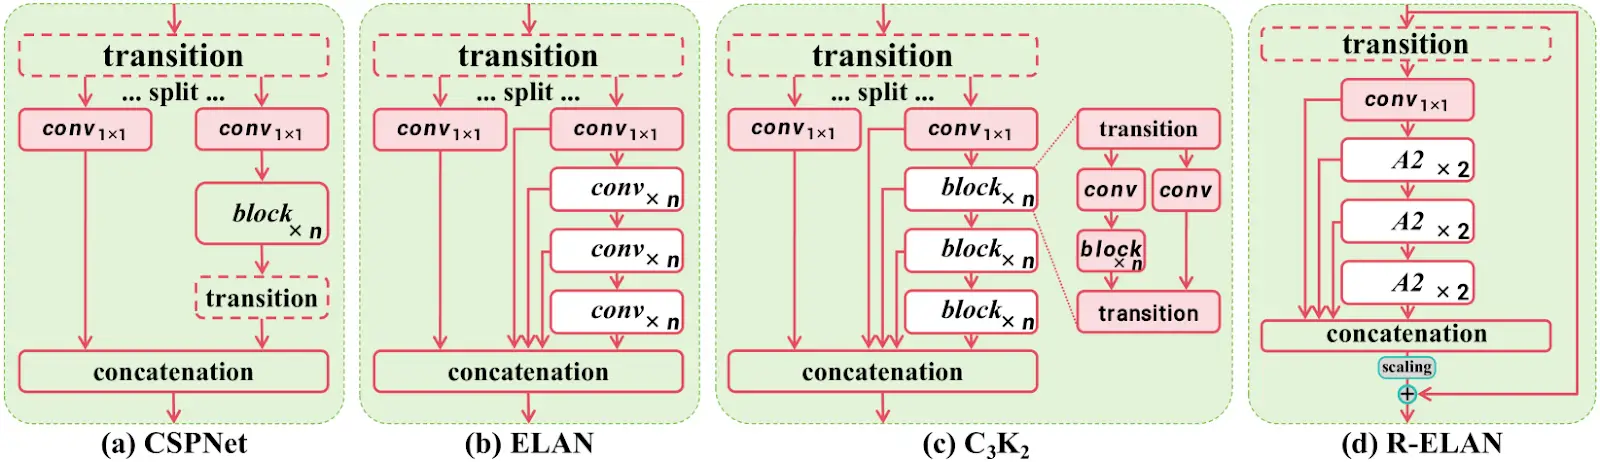
\includegraphics[scale=0.18]{gambar/r elan.png}
  % Keterangan gambar yang diinputkan
  \caption{Blok diagram dari sistem}
  % Label referensi dari gambar yang diinputkan
  \label{fig:rancangan penelitian}
\end{figure}

Blok R ELAN berisi lapisan convolusi (1x1) transition layer yang berfungsi untuk mereduksi input, lalu dilanjutkan dengan split feature map yang digunakan untuk memisahkan fitur ke beberapa bagian, lalu dilanjutkan ke lapisan convolusi (3x3) yang telah di stack untuk mengekstraksi fitur secara mendalam, lalu ada shortcut yang menghubungkan input dan output, dan diakhiri dengan lapisan concat yang menghubungkan semua output tersebut kedalam satu tensor. Dengan penggabungan setiap lapisan tersebut menghasilkan blok yang memiliki fungsi untuk memaksimalkan pemrosesan fitur sambil menjaga stabilitas pelatihan, dengan struktur residual dan strategi agregasi efisien.

\subsection{Preprocessing}
Setelah citra diklasifikasi maka akan dilakukan Preprocessing yang menghasilkan jarak dari citra yang didapatkan. Adapun proses ini melibatkan perhitungan dari nilai nilai yang didapatkan dari bounding box dalam layar, Seperti tinggi bounding box dalam pixel maupun lebar bounding box dalam pixel.

Untuk mendapatkan jarak menggunakan bounding box dengan menerapkan konsep Fokus Panjang dalam Pixel \emph{Focal Length Pixel}. Adapun fokus panjang dalam pixel ini adalah konversi dari fokus panjang lensa kamera  yang biasanya diukur dalam meter ke dalam satuan pixel. Konsep ini biasa digunakan dalam visi komputer untuk menghubungkan informasi visual dari kamera ke ukuran fisik di dunia nyata. Adapun rumus Fokus panjang dalam pixel dapat dilihat pada rumusan berikut

\begin{equation}
    f_p = \frac{D \times h_b}{H-o}
\end{equation}

Dimana :
\begin{itemize}
    \item $f_p$ adalah \emph{focal length pixel}.
    \item $D$ adalah jarak sebenarnya dari kamera ke objek.
    \item $h_b$ adalah tinggi bounding box dalam piksel.
    \item $H_o$ adalah tinggi sebenarnya dalam objek.
\end{itemize}

Dengan mendapatkan nilai $f_p$ kita dapat mengkonversi pengukuran dari ruang gambar (piksel) ke dimensi dunia nyata (meter atau centimeter). Nilai tinggi rata rata manusia juga digunakan untuk melakukan konversi. Adapun rumus konversinya sebagai berikut

\begin{equation}
    D = \frac{f_p \times H_o}{h_b}
\end{equation}

Dimana :
\begin{itemize}
    \item $H_o$ merupakan tinggi rata - rata manusia
\end{itemize}

Jarak yang didapatkan sekarang dapat digunakan dalam sistem braking yang akan diimplementasikan di kursi roda. Dimana pada proyek kali ini digunakan Jarak 1.3 meter sebagai syarat kursi roda untuk berhenti. Yang mana apabila sudah dijarak 1.3 meter maka kursi roda akan berhenti.

\subsection{Input Citra LSTM}
Pada tahap ini, diawali dengan pengambilan citra untuk dataset. Pengambilan dataset dilakukan langsung melalui kursi roda dengan menggunakan kamera yang menghadap ke pengguna kursi roda. 
\begin{figure} [H] \centering
  % Nama dari file gambar yang diinputkan
  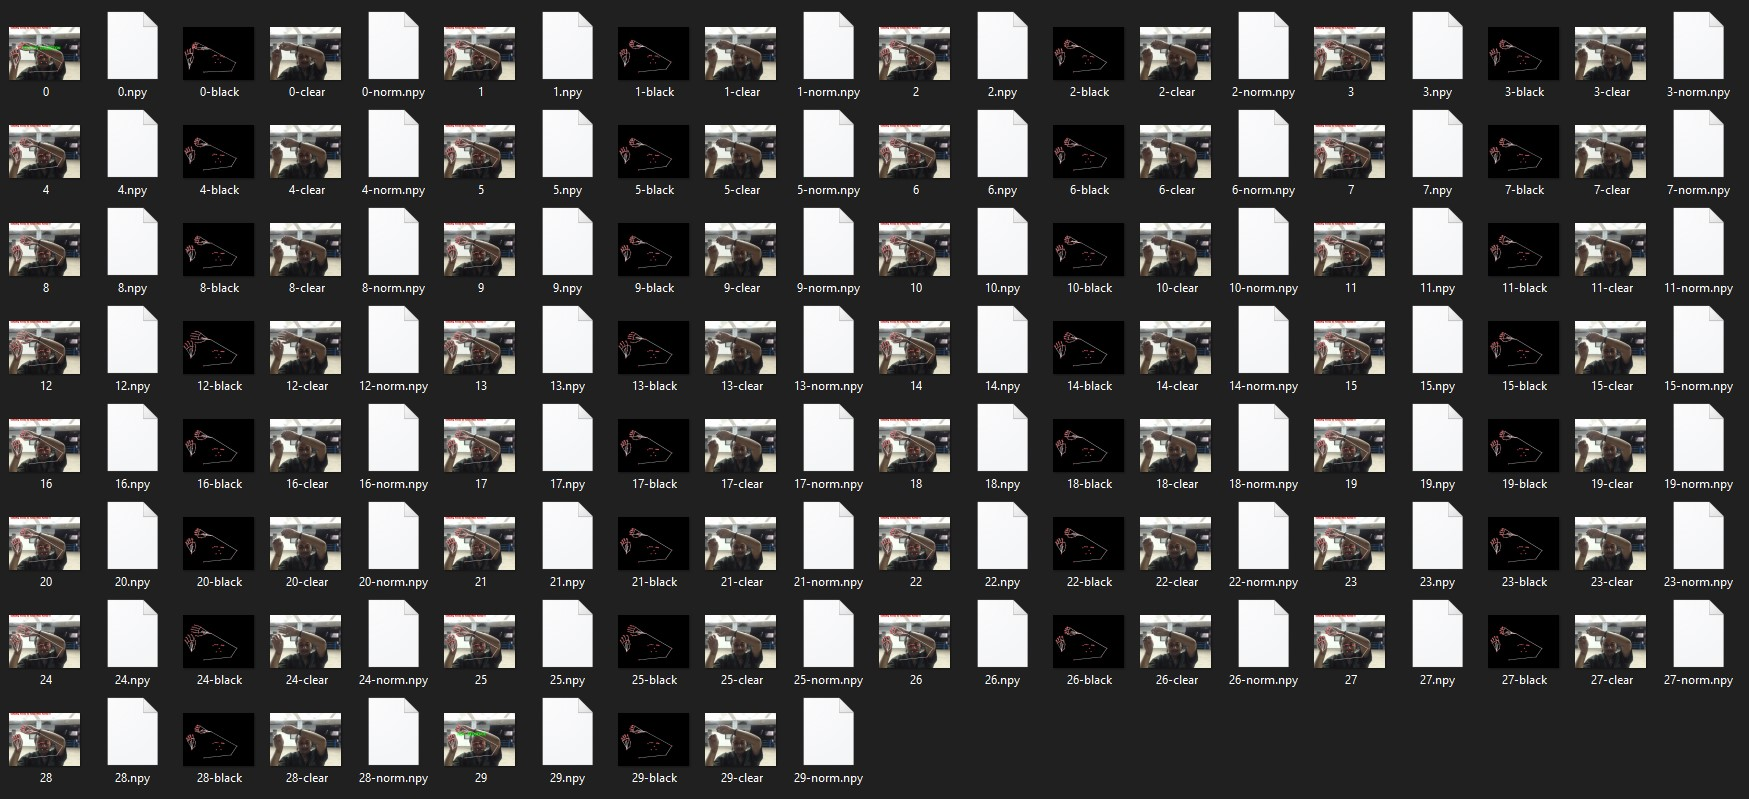
\includegraphics[scale=0.28]{gambar/dataset.jpg}
  % Keterangan gambar yang diinputkan
  \caption{Dataset untuk gestur kanan}
  % Label referensi dari gambar yang diinputkan
  \label{fig:gestur dataset}
\end{figure}

Data citra kedua merupakan input YOLO untuk mendeteksi objek yang ada di depan kursi roda. Data citra ini akan digunakan untuk pendeteksian objek penghalang di depan kursi roda yang berguna untuk \emph{braking system} dari kursi roda
\begin{figure} [H] \centering
  % Nama dari file gambar yang diinputkan
  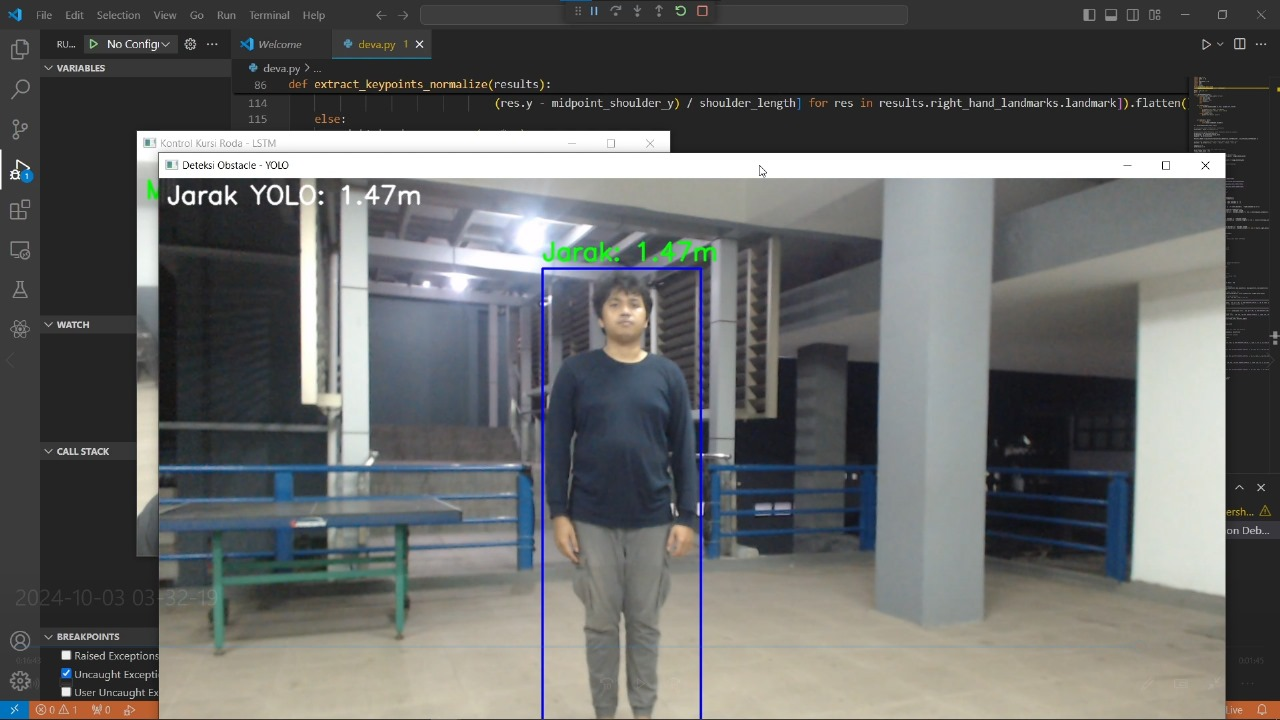
\includegraphics[scale=0.35]{gambar/yolo.jpg}
  % Keterangan gambar yang diinputkan
  \caption{Hasil deteksi YOLO}
  % Label referensi dari gambar yang diinputkan
  \label{fig:citra yolo}
\end{figure}

\subsection{Ekstraksi Fitur}
Ekstraksi fitur dalam program LSTM (Long Short-Term Memory) adalah proses pengambilan informasi penting dari data mentah untuk digunakan sebagai input bagi model. Proses ini bertujuan untuk menyederhanakan data dan menyoroti pola atau karakteristik relevan yang dapat membantu model memahami hubungan temporal dalam data berurutan seperti teks, sinyal, atau deret waktu. Metode ekstraksi fitur bisa dilakukan secara manual, misalnya dengan menghitung statistik dasar seperti rata-rata atau transformasi sinyal seperti FFT, atau secara otomatis menggunakan model pembelajaran mendalam untuk menghasilkan representasi numerik, seperti word embeddings untuk teks atau representasi vektor dari gambar. Dalam konteks LSTM, fitur-fitur yang telah diekstraksi ini diorganisasi dalam urutan yang sesuai dengan waktu atau konteks data, sehingga LSTM dapat mempelajari hubungan temporal antar fitur secara efektif. Dengan ekstraksi fitur yang tepat, model LSTM dapat bekerja lebih efisien, menghasilkan kinerja yang lebih baik dengan memanfaatkan informasi relevan dan mengurangi gangguan dari data mentah.

\subsection{Normalisasi}
Normalisasi adalah proses transformasi data untuk menyelaraskan nilai-nilainya dalam rentang tertentu atau membuat distribusinya konsisten, sehingga mempermudah analisis dan meningkatkan kinerja model pembelajaran mesin. Proses ini bertujuan untuk mengurangi pengaruh skala fitur yang besar terhadap model, mempercepat konvergensi selama pelatihan, dan mencegah dominasi fitur tertentu. Metode normalisasi yang umum meliputi Min-Max Scaling, yang mengubah nilai ke rentang tertentu seperti 0 hingga 1, dan Z-Score Normalization, yang menyelaraskan data sehingga memiliki rata-rata 0 dan standar deviasi 1. Misalnya, dalam citra digital, normalisasi dilakukan dengan mengubah nilai piksel dari skala 0-255 menjadi 0 hingga 1 agar lebih mudah diproses oleh model. Dengan normalisasi, semua fitur dalam data berada pada skala yang seimbang, memungkinkan algoritma pembelajaran mesin untuk lebih fokus pada pola dan hubungan dalam data tanpa terganggu oleh perbedaan skala antar fitur.

\subsection{Klasifikasi Gestur}
Pada tahap ini, gestur yang sudah diambil selanjutnya diklasifikasikan sesuai dengan perintah yang ada pada kursi roda. Terdapat 5 kelas yang digunakan yang kelas maju, kelas mundur, kelas kanan, kelas kiri, dan kelas stop.

\subsection{Braking System}
Klasifikasi dari YOLO nantinya akan digunakan untuk melakukan \emph{braking} otomatis jika mendeteksi kelas yang ditentukan, dalam penelitian ini kelas yang digunakan adalah manusia. Jarak untuk menentukan \emph{braking} adalah 1.3 meter. Jika dalam jarak 1.3 meter terdeteksi manusia maka kursi roda akan berhenti secara otomatis, ini berguna untuk mengurangi resiko kecelakaan pengguna kursi roda.
\subsection{Motion Command}
Motion command adalah perintah yang digunakan untuk mengendalikan gerakan suatu objek atau perangkat, seperti kursi roda, dengan memberikan instruksi terkait arah, kecepatan, atau posisi yang harus dicapai. Dalam konteks penelitian ini, motion command berfungsi untuk mengubah input gestur menjadi perintah gerakan yang spesifik untuk kursi roda. Setiap kelas yang Anda gunakan (A, B, C, D, dan E) mewakili jenis perintah gerakan yang berbeda: Kelas A untuk bergerak ke kiri, kelas B untuk bergerak maju, kelas C untuk berhenti, kelas D untuk bergerak mundur, dan kelas E untuk bergerak ke kanan. Setelah sistem mendeteksi gestur yang sesuai, seperti gerakan tangan atau tubuh, hasil klasifikasi tersebut diterjemahkan menjadi motion command yang dikirim ke sistem kendali kursi roda. Perintah ini kemudian dieksekusi oleh motor atau aktuator kursi roda untuk melaksanakan gerakan yang diinginkan. Dengan menggunakan motion command yang terhubung langsung ke kelas gestur, sistem dapat mengendalikan kursi roda secara responsif dan akurat berdasarkan input dari pengguna.

\subsection{Motion Planning}
Motion planning adalah proses perencanaan jalur atau gerakan bagi suatu objek atau perangkat untuk mencapai tujuan tertentu dengan mempertimbangkan berbagai faktor, seperti hambatan, batasan kecepatan, dan kondisi lingkungan. Dalam konteks robotika atau kendaraan otonom, motion planning bertujuan untuk merencanakan serangkaian langkah atau aksi yang harus diambil agar objek dapat bergerak dari titik awal menuju titik tujuan secara aman, efisien, dan sesuai dengan batasan yang ada. Proses ini melibatkan pembuatan peta lingkungan yang menggambarkan hambatan yang harus dihindari, serta perencanaan jalur yang menghubungkan posisi awal dan tujuan. Selain itu, motion planning juga mencakup optimasi jalur untuk meningkatkan efisiensi, seperti mengurangi waktu atau energi yang dibutuhkan, dan eksekusi jalur tersebut dengan mengontrol perangkat untuk mengikuti rute yang telah direncanakan. Dalam kendaraan otonom, misalnya, motion planning digunakan untuk merencanakan jalur yang menghindari kendaraan lain dan rintangan di jalan, sementara dalam robotika, motion planning memastikan robot dapat bergerak dari satu lokasi ke lokasi lain tanpa menabrak objek sekitarnya. Dengan demikian, motion planning memungkinkan perangkat bergerak secara cerdas, aman, dan responsif terhadap lingkungan sekitarnya.

\newpage
\subsection{Training Model}
Pada tahap ini, dataset yang sudah diklasifikasi selanjutnya akan masuk ke tahap training ke sel LSTM.
\begin{figure} [H] \centering
  % Nama dari file gambar yang diinputkan
  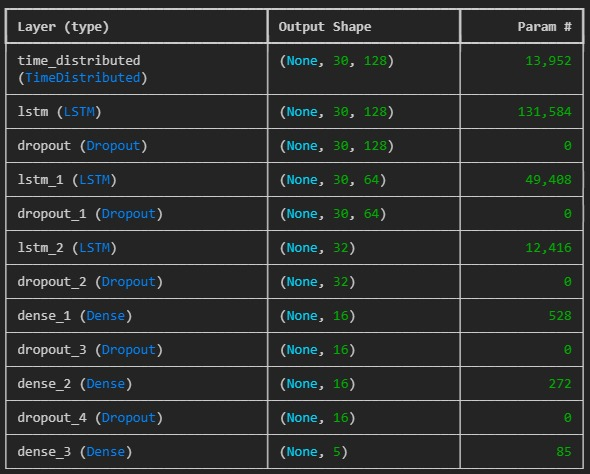
\includegraphics[scale=0.6]{gambar/training model.jpg}
  % Keterangan gambar yang diinputkan
  \caption{Struktur LSTM untuk Training Gestur Tangan}
  % Label referensi dari gambar yang diinputkan
  \label{fig:training model}
\end{figure}
Proses dimulai dengan lapisan TimeDistributed, yang menerapkan transformasi pada setiap langkah waktu dari data sekuensial dengan panjang 30, menghasilkan keluaran dengan dimensi 128. Lapisan ini digunakan untuk mengolah data dengan fitur per frame, seperti hasil dari pose estimation. Selanjutnya, lapisan LSTM pertama memproses data sekuensial untuk menangkap pola temporal dengan keluaran 128 per langkah waktu, diikuti dengan lapisan Dropout untuk mencegah overfitting. Lapisan LSTM kedua mengurangi dimensi keluaran menjadi 64 unit untuk fokus pada pola yang lebih signifikan, diikuti oleh Dropout kedua. LSTM ketiga mengurangi dimensi menjadi 32 unit untuk mempertahankan informasi penting, dengan Dropout ketiga untuk menjaga generalisasi. Setelah itu, lapisan Dense pertama mengintegrasikan informasi dari lapisan sebelumnya dengan 16 unit, diikuti dengan Dropout untuk regularisasi. Lapisan Dense kedua juga memiliki 16 unit untuk memperdalam pengolahan informasi, disertai dengan Dropout keempat. Lapisan Dense ketiga, yang merupakan lapisan output, menghasilkan 5 neuron yang kemungkinan mewakili 5 kelas gestur atau tindakan berbeda. Dengan penggunaan Dropout di setiap tahap, model ini dirancang untuk mencegah overfitting dan meningkatkan generalisasi agar dapat bekerja dengan baik pada data baru.

\newpage
\section{Hardware}
pada tahap ini, perancangan hardware dilakukan sesuai dengan alur yang telah direncanakan sebelumnya. Perancangan ini akan dipresentasikan dengan blok diagram alur yang telah mereprentasikan alur dari bagian hardware.
\begin{figure} [H] \centering
  % Nama dari file gambar yang diinputkan
  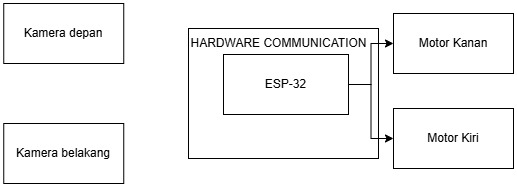
\includegraphics[scale=0.6]{gambar/hardware new.jpg}
  % Keterangan gambar yang diinputkan
  \caption{Diagram Hardware}
  % Label referensi dari gambar yang diinputkan
  \label{fig:hardware}
\end{figure}

\subsection{Kamera Depan}
Kamera depan berfungsi sebagai hardware untuk mengambil citra untuk YOLO yang akan mendeteksi objek manusia. Setelah citra diproses, YOLO akan membagi gambar menjadi grid dan menghasilkan prediksi berupa bounding box, label kelas, dan skor probabilitas untuk setiap objek yang terdeteksi. Dengan cara ini, kursi roda atau sistem dapat mengidentifikasi objek di jalur depan dan berhenti ketika mendeteksi manusia. Kamera depan berfungsi sebagai "mata" sistem untuk memberikan informasi visual yang diperlukan bagi YOLO untuk melakukan deteksi objek secara real-time.

\subsection{Kamera Belakang}
Kamera belakang berfungsi sebagai input citra untuk LSTM. Prosesnya dimulai dengan kamera belakang yang menangkap citra atau video dari pengguna kursi roda. MediaPipe akan menganalisis citra tersebut dan mendeteksi landmark tubuh, misalnya posisi tangan yang kemudian diterjemahkan menjadi input untuk model LSTM. LSTM akan memproses urutan data ini, memahami pola gerakan atau posisi tubuh pengguna, dan menghasilkan output yang sesuai, seperti perintah untuk menggerakkan kursi roda maju, mundur, atau berbelok. Dengan menggunakan LSTM, model dapat mengingat dan merespons gerakan tubuh sebelumnya, memberikan kontrol yang lebih lancar dan alami atas kursi roda, berdasarkan input gestur atau posisi tubuh yang terdeteksi oleh kamera belakang.
\subsection{Laptop}
Pada tahap awal, data di peroleh dengan menggunakan kamera yang dipasang pada bracket khusus. Desain bracket ini memungkinkan kamera untuk menangkap citra tangan dengan sudut pandang yang optimal, sehingga memastikan pengambilan gambar yang akurat. Proses ini melibatkan pengambilan gambar dan video secara real-time, yang sangat penting untuk memastikan data yang dihasilkan relevan dan dapat digunakan untuk analisis lebih lanjut.

Setelah citra berhasil dikumpulkan, langkah berikutnya adalah pengolahan data tersebut dengan melakukan klasifikasi menggunakan Model LSTM yang telah dilatih sebelumnya, yang disimpan dalam format .h5. Model ini digunakan untuk mendeteksi gestur yang terdeteksi dalam citra. Untuk mendukung proses ini, beberapa library perlu diinstal terlebih dahulu, dan instalasinya dilakukan melalui serangkaian perintah yang telah ditentukan. Adapun penggunaan library yang akan digunakan ialah, Mediapipe, Scikit - learn, tensor-
flow, keras, seaborn, numpy dan opencv-python. Library - library ini memastikan semua alat dan dependensi yang diperlukan untuk menjalankan model tersebut pada perangkat laptop.

Spesifikasi laptop yang digunakan dalam penelitian ini adalah laptop ROG Strix G512LU dengan spesifikasi sebagai Tabel berikut:
\begin{table}[ht]
\centering
\begin{tabular}{|c|c|}
\hline
\textbf{Spesifikasi} & \textbf{Detail} \\ \hline
CPU & Intel Core I7-10750H \\ \hline
RAM & 16 GB DDR4\\ \hline
GPU & GTX 1660 Ti \\ \hline
\end{tabular}
\caption{Spesifikasi Laptop}
\label{tab:spec_laptop}
\end{table}
Pada tugas akhir ini, data citra tangan yang telah diproses dan diklasifikasikan akan menghasilkan perintah yang dikirimkan dari laptop ke ESP32 melalui koneksi WiFi. Pengiriman data ini sangat penting karena hasil klasifikasi akan digunakan untuk mengendalikan motor pada kursi roda, memungkinkan kursi roda dikendalikan melalui gestur tangan.

Untuk memastikan pengiriman data berjalan lancar, laptop harus terlebih dahulu terhubung ke access point yang disediakan oleh ESP32. Proses ini melibatkan konfigurasi koneksi WiFi pada laptop agar dapat berkomunikasi dengan ESP32. Setelah koneksi berhasil, data klasifikasi mulai dikirim. Pengiriman data dilakukan menggunakan bahasa pemrograman Python, yang dipilih karena fleksibilitasnya dalam menangani operasi jaringan dan pengolahan data. Data dikirim dalam format string, yang sederhana namun efektif untuk transmisi data melalui jaringan.

Untuk membangun koneksi jaringan yang memungkinkan pengiriman dan penerimaan data, digunakan beberapa library Python seperti socket, time, dan datetime. Library socket menangani komunikasi jaringan, memungkinkan program untuk mengirim dan menerima data melalui koneksi TCP/IP. Library time digunakan untuk mengatur interval pengiriman data, memastikan data dikirim pada waktu yang tepat. Sementara itu, library datetime mencatat waktu pengiriman data untuk keperluan logging dan debugging.

IP Address dari access point ESP32 digunakan sebagai variabel host dalam program, sementara port 80 digunakan sebagai variabel port. Port 80 adalah port standar untuk komunikasi HTTP, yang memungkinkan penggunaan protokol HTTP untuk pengiriman data. Setelah semua konfigurasi selesai, program akan menghubungkan ke server sesuai dengan IP Address dan port yang telah ditentukan, memastikan pengiriman data dari laptop ke ESP32 berjalan dengan lancar.Program ini dirancang untuk berjalan secara terus-menerus, menerima input dari pengguna dan mengirimkan data ke ESP32 tanpa batas waktu.

\subsection{ESP-32}
Pada ESP-32 akan menerima data dari laptop untuk memberikan perintah pada kursi roda sesuai dengan kelas yang dipanggil secara \emph{real-time}. Program dimulai dengan mengimpor beberapa library yang diperlukan untuk menjalankan berbagai fungsi, seperti WiFi, Arduino, dan JSON. Library WiFi digunakan untuk mengelola koneksi jaringan, library Arduino untuk mengontrol perangkat keras, dan library JSON untuk memproses data dalam format JSON. Setelah itu, dilakukan inisialisasi pada komunikasi serial, WiFi, dan server untuk memastikan bahwa ESP32 siap menerima dan mengirimkan data melalui jaringan.

Selanjutnya, program memeriksa apakah ada perangkat yang terhubung ke server ESP32 dengan menggunakan fungsi pemeriksa koneksi jaringan. Jika tidak ada perangkat yang terhubung, program akan terus memeriksa hingga perangkat berhasil terhubung. Setelah perangkat terhubung, program akan memeriksa apakah ada data yang dikirimkan. Jika ada data yang diterima, program akan masuk ke dalam loop untuk membaca data secara terus-menerus. Data yang diterima kemudian akan disimpan dalam variabel \texttt{receivedData}, dan string data akan dibaca hingga ditemukan karakter newline (/n), yang menandakan akhir dari data tersebut.
Setelah data diterima dan disimpan, string data tersebut akan diekstraksi untuk mendapatkan informasi mengenai arah dan kecepatan. Proses ekstraksi ini sangat penting untuk mengonversi string data menjadi format yang dapat digunakan oleh program untuk mengendalikan motor pada kursi roda. Setelah ekstraksi selesai, data arah dan kecepatan yang telah diproses akan ditampilkan guna memastikan bahwa informasi yang diterima sesuai dengan yang diharapkan. Dengan data arah dan kecepatan yang sudah tersedia, ESP32 dapat mengirimkan instruksi ke motor kursi roda agar bergerak sesuai dengan perintah yang diterima. Proses ini akan terus berulang selama perangkat tetap terhubung dan data terus diterima. Berikut merupakan perintah sesuai dengan kelas yang dipanggil:

\begin{table}[H]
    \centering
    \begin{tabular}{|c|c|}
    \hline
    \textbf{Klasifikasi gestur} & \textbf{Kode Intruksi} \\ \hline
    Kiri & A \\ \hline
    Maju & B \\ \hline
    Stop & C \\ \hline
    Mundur & D \\ \hline
    Kanan & E \\ \hline
    \end{tabular}
    \caption{Kode Instruksi dari hasil klasifikasi}
    \label{tab:kode intruksi}
\end{table}

Sesuai dengan Tabel 3.2, kode intruksi tersebut diimplementasikan dengan hasil gestur yang didapatkan dari hasil training LSTM. Pengoperasian dari kursi roda diawali dengan intruksi kode B yakni maju, jika pengguna mengintruksikan kode A atau E kursi roda akan berbelok ke kiri atau kanan. Namun perlu diperhatikan, apabila ingin berganti arah agar motor tidak mengalami kesalahan dalam menerima input yang dihasilkan model, maka perlu dilakukan pemanggilan kelas ’Stop’ atau mengirim instruksi ’C’.

\newpage
\subsection{Skematik Alat}
\begin{figure} [H] \centering
  % Nama dari file gambar yang diinputkan
  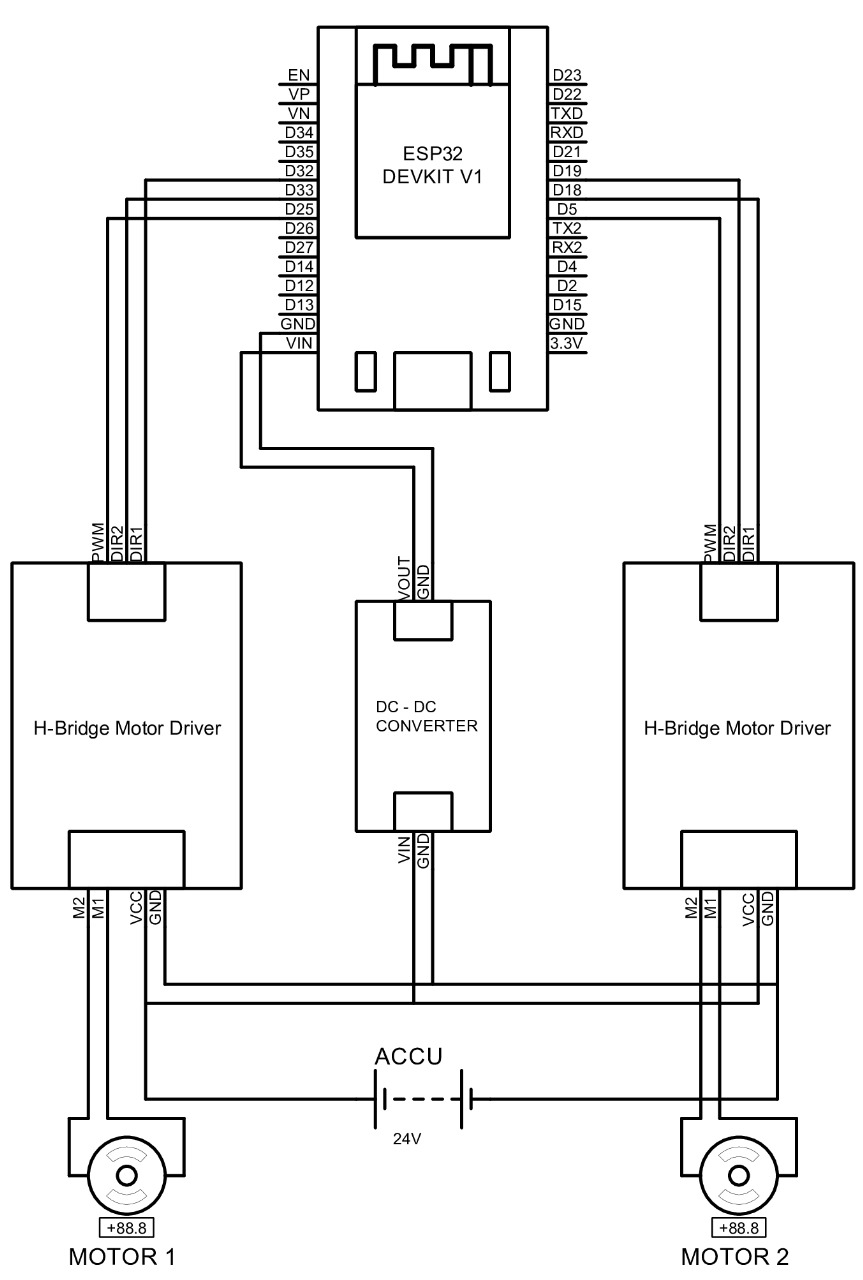
\includegraphics[scale=0.4]{gambar/skematik alat.jpg}
  % Keterangan gambar yang diinputkan
  \caption{Skematik kontrol motor kursi roda\cite{ekatama2024perancangan}}
  % Label referensi dari gambar yang diinputkan
  \label{fig:skematik kontrol}
\end{figure}

Dari penelitian yang telah dilakukan, telah dirancang sebuah sistem kontrol untuk motor
kursi roda dengan skematik alat yang ditampilkan pada Gambar 3.8. ESP32 akan terhubung
dengan dua buah H-Bridge Motor Driver dan sebuah DC-DC Converter. Setiap H-Bridge Mo-
tor Driver terhubung langsung ke motor roda kiri dan motor roda kanan untuk menggerakkan
roda kursi roda secara efektif. Dalam skematik ini, ESP32 berfungsi sebagai otak dari sistem, mengirimkan sinyal kontrol ke motor driver berdasarkan data yang diterima melalui koneksi WiFi\cite{ekatama2024perancangan}.

 Program dirancang untuk mengendalikan motor DC dengan memproses perintah yang dikirim melalui jaringan WiFi. Tahapan pertama dalam program adalah mengimpor library yang dibutuhkan, seperti Arduino dan WiFi, untuk menyediakan fungsi-fungsi penting. Setelah itu, dilakukan inisialisasi PWM dan konfigurasi pin sebagai saluran untuk mengirim sinyal kontrol ke motor driver.

Setelah inisialisasi selesai, program mulai memeriksa koneksi dengan perangkat yang terhubung ke server ESP32. Jika belum ada perangkat yang terhubung, program akan terus memantau hingga koneksi berhasil. Ketika koneksi berhasil, program melanjutkan dengan memeriksa apakah ada data yang diterima dari perangkat tersebut. Jika data ditemukan, program membacanya hingga mendeteksi karakter newline (/n), yang menunjukkan akhir dari string data.

Data yang diterima selanjutnya diproses untuk mengekstrak informasi mengenai arah dan kecepatan. Tahap ini mengubah string data menjadi format yang dapat digunakan oleh program untuk mengontrol motor kursi roda. Berdasarkan informasi ini, ESP32 mengirimkan instruksi ke motor driver untuk menggerakkan roda sesuai arah dan kecepatan yang diinginkan.

Sistem kontrol kursi roda ini menggunakan dua metode pengendalian. Metode pertama adalah differential drive, di mana roda kanan bergerak mundur dan roda kiri maju saat berbelok ke kanan, serta sebaliknya untuk berbelok ke kiri. Metode kedua adalah gerakan normal, di mana roda kanan diam dan roda kiri bergerak maju saat berbelok ke kanan, atau sebaliknya saat berbelok ke kiri. Saat bergerak maju atau mundur, kedua roda berputar serentak ke arah yang sama. Dalam penelitian ini, metode kedua dipilih untuk mengendalikan pergerakan kursi roda.

Program ini memastikan ESP32 dapat berfungsi secara optimal sebagai pengontrol motor. Setiap langkah dalam flowchart dirancang untuk memastikan sistem bekerja dengan efisien dan responsif terhadap perintah yang diterima melalui jaringan WiFi. Dengan pengoperasian secara real-time, sistem mampu merespons perintah dengan cepat dan memberikan kontrol yang presisi untuk pergerakan kursi roda\cite{ekatama2024perancangan}.
\cleardoublepage
\chapter{PENGUJIAN DAN ANALISIS}
Pada bab ini, akan dijelaskan mengenai hasil dari pengujian dan analisis dari penelitian yang telah diuraikan pada metodologi. Selain itu, akan dipaparkan mengenai skenario dari pengujian yang dilakukan untuk evaluasi performa dari sistem. Pengujian ini dilakukan untuk memastikan bahwa sistem yang telah dirancang mampu berfungsi dengan baik dan situasi yang mungkin dihadapi oleh pengguna.
\section{Skenario Pengujian}
Pengujian dilakukan untuk menguji performa dari model dalam melakukan deteksi terhadap gestur untuk sistem kendali dan sistem pengereman otomatis. Skenario pengujian dirancang untuk mengukur berbagai aspek dari sistem seperti akurasi deteksi terhadap kelas yang dipanggil, \emph{respond time}, kecepatan pemrosesan, dan respon sistem terhadap objek di depannya yang berpengaruh kepada pengereman otomatis. Skenario pengujian yang dilakukan adalah sebagai berikut;
\begin{enumerate}
    \item Hasil Pengujian model
    \item Pengujian berdasarkan FPS
    \item Pengujian berdasarkan hasil \emph{respond time}
    \item Pengujian terhadap akurasi dari kelas yang dipanggil
    \item Pengujian sistem pengereman otomatis pada jarak 150 cm
    \item Pengujian sistem pengereman otomatis pada jarak 130 cm
    \item Pengujian sistem pengereman otomatis pada jarak 100 cm
\end{enumerate}
\section{Pengujian Performa Model YOLOv11 Menggunakan Confusion Matrix}
Data yang digunakan sebagai set data berjumlah 5372 citra manusia dengan perbandingan 4359 set data train dan 1023 set data validasi. Setelah proses pemuatan set dilakukan di lanjutkan dengan proses pelatihan model.
Proses pelatihan dilakukan dengan beberapa parameter yang nantinya akan diuji, yang dimana parameter ini akan dibandingkan performanya melalui nilai confusion matrix maupun nilai akurasi deteksi seperti skor mAP, precision, box loss.
Gambar 4.1 merupakan input layer yang digunakan.
\begin{figure} [H] \centering
  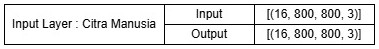
\includegraphics[scale=0.65]{gambar/Input layer.jpg}
  \caption{Input Layer Pelatihan}
  \label{fig:Pengujian Performa}
\end{figure}
Pelatihan pertama menggunakan 150 epoch. Input layer memiliki batch size sebesar 16 dengan tindakan praproses merubah ukuran gambar pada dataset menjadi 800x800 piksel. Adapun tujuan dari pelatihan ini untuk mengetahui seberapa baik peningkatan model pre- trained
yang digunakan dalam deteksi manusia berdasarkan jumlah Epoch yang ditentukan. Berikut nilai box loss yang didapatkan dari hasil training pada Gambar 4.2
\begin{figure} [H] \centering
  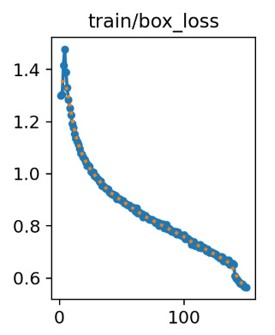
\includegraphics[scale=0.55]{gambar/train box loss.jpg}
  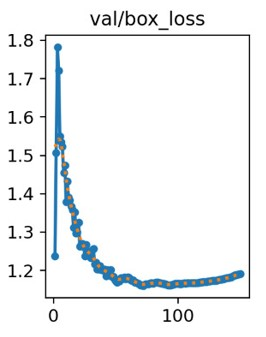
\includegraphics[scale=0.55]{gambar/val box loss.jpg}
  \caption{Grafik \emph{box loss}}
  \label{fig:Pengujian Performa}
\end{figure}
Didapatkan nilai dari \emph{box loss} pada hasil pelatihan YOLOv11 adalah sebesar 0.598
setelah 150 epoch. \emph{Box loss} mengukur seberapa baik model memprediksi bounding
box di sekitar objek. Tujuan dari loss ini adalah untuk mengoptimalkan model
agar bounding box yang diprediksi sesuai dengan posisi dan ukuran objek sebenarnya dalam gambar.
Adapun penurunan yang terlihat pada gambar pelatihan box loss menandakan bahwa hasil
pelatihan yang dilakukan telah berhasil membuat model menentukan koordinat \emph{bounding box}
pada objek manusia secara akurat.

Nilai dari \emph{box loss} pada proses validasi menggunakan YOLOv11 ini adalah 1.21,
\emph{box loss} validasi ini mengindikasi kemampuan mengenali objek pada data uji. Secara teori
, penurunan objek loss pada tahap validasi menandakan bahwa objek mampu melakukan deteksi
secara umum. Namun diakhir terlihat grafik sedikit naik. Hal ini menandakan ketika model
mulai menghafal pola data training dengan baik, tapi gagal menggeneralisasi pada data validasi.
Akibatnya, \emph{loss training} tetap atau terus menurun, loss validasi justru naik sedikit karena
model tidak mampu memprediksi data validasi dengan baik. Selanjutnya grafik dari mAP dapat dilihat
pada Gambar 4.3
\begin{figure} [H] \centering
  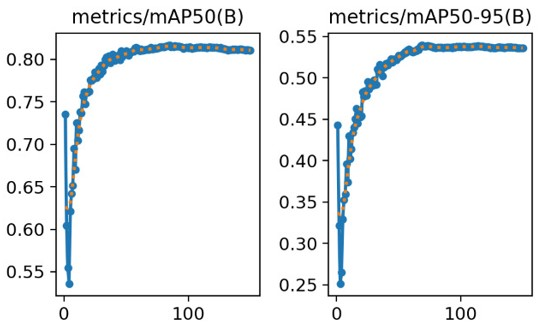
\includegraphics[scale=0.63]{gambar/map grafik yolov11.jpg}
  \caption{Grafik mAP epoch 150}
  \label{fig:Pengujian Performa}
\end{figure}
Skor mAP50 pada \emph{threshold} 0.5 yang diperoleh dari proses ini adalah sebesar 0.812, ini mengindikasikan
bahwa model memiliki kemampuan yang sangat baik dalam mendeteksi objek dengan kecepatan tinggi,
syarat minimal dari kriteria IoU adalah 0.5 terpenuhi. Hal ini menunjukan bahwa dalam percobaan kasus, \emph{bounding box}
yang diprediksi oleh model memiliki kesesuaian yang signifikan dengan \emph{bounding box ground truth}. 

Pada grafik mAP50-95 dengan prediksi yang lebih presisi. Nilai mAP50-95 adalah 0.25 diawal dan mulai terlihat kenaikan yang 
signifikan mencapai 0.543 di epoch ke 78. Hal ini menunjukan bahwa walaupun model sudah mampu mendeteksi objek dengan cukup
baik pada \emph{threshold} rendah, namun masih terdapat tantangan dalam mempertahankan akurasi deteksi
saat persyaratan presisi yang tumpang tindih semakin ketat.

Berikut merupakan grafik dari hasil yang didapatkan secara keseluruhan dari pealtihan model YOLOv11.
Pada Gambar 4.4 merupakan grafik hasil yang didapatkan pada model secara keseluruhan.
Didapatkan nilai- nilai pada masing masing grafik, pada train box loss didapatkan nilai 0.598,
pada train cls loss didapatkan nilai 0.412, pada train dfl loss didapatkan nilai 0.901 , pada
metrics precision didapatkan nilai 0.878, pada grafik recall 0.748, pada val box loss didapatkan nilai 1.211, pada val
cls loss didapatkan nilai 0.793, dan pada val dfl loss didapatkan nilai 1.342,  pada grafik mAP50
0.812, pada grafik mAP50-95 0.543

\begin{figure} [H] \centering
  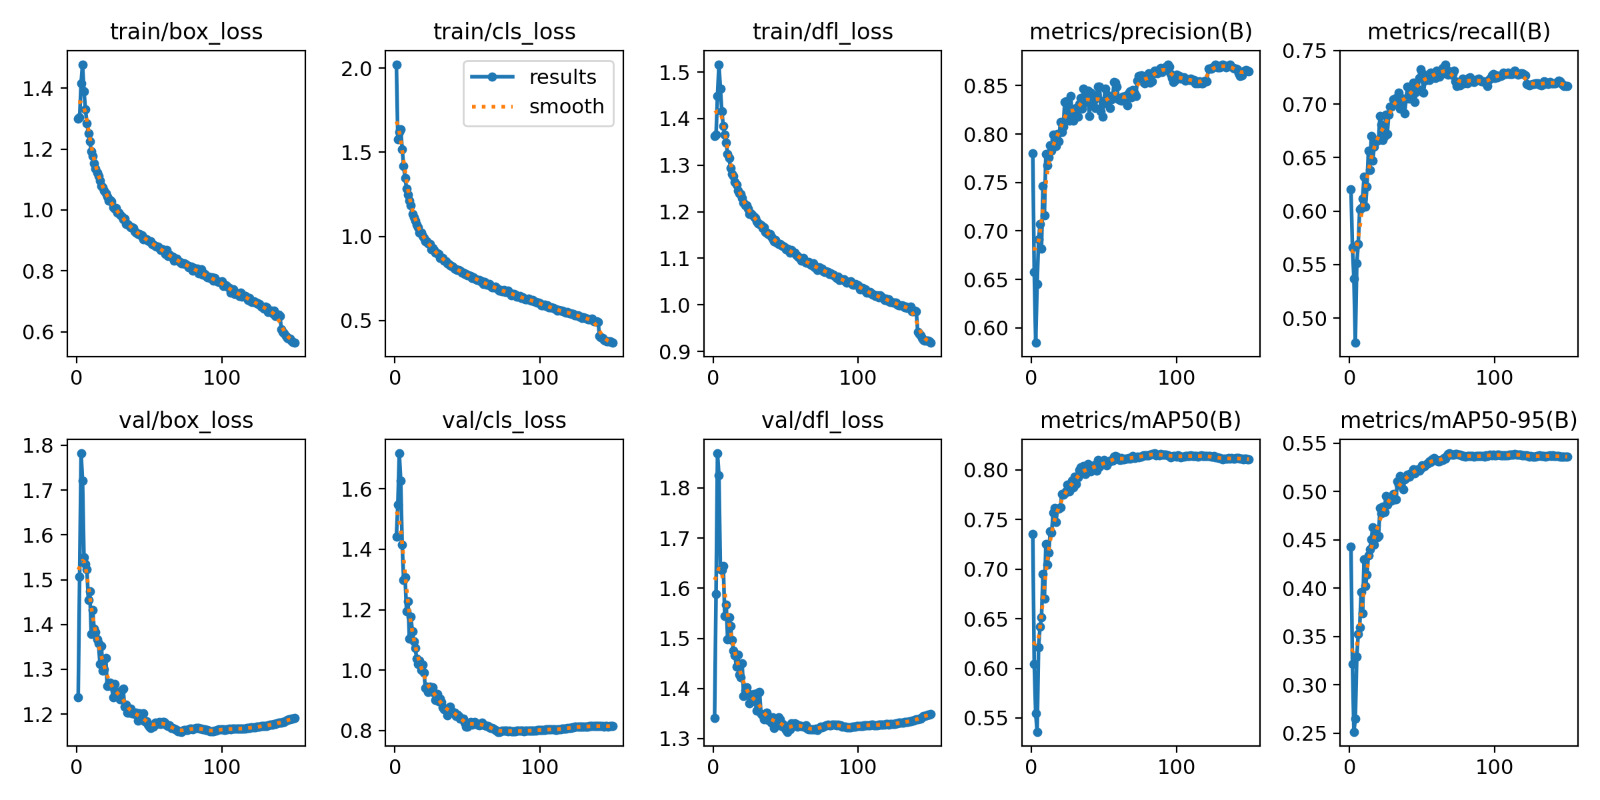
\includegraphics[scale=0.23]{gambar/Hasil.jpg}
  \caption{Grafik keseluruhan pelatihan epoch 150}
  \label{fig:Pengujian Performa}
\end{figure}

Berikut adalah visualisasi melalui \emph{confusion matrix} terkait dengan pelatihan model YOLOv11 dengan 150 epoch.
Pada Gambar 4.5 indikator yang digunakan pada \emph{confusion matrix} pada setiap kotaknya merepresentasikan nilai \emph{true positive, false positive, false negative, true negative}.
\begin{figure} [H] \centering
  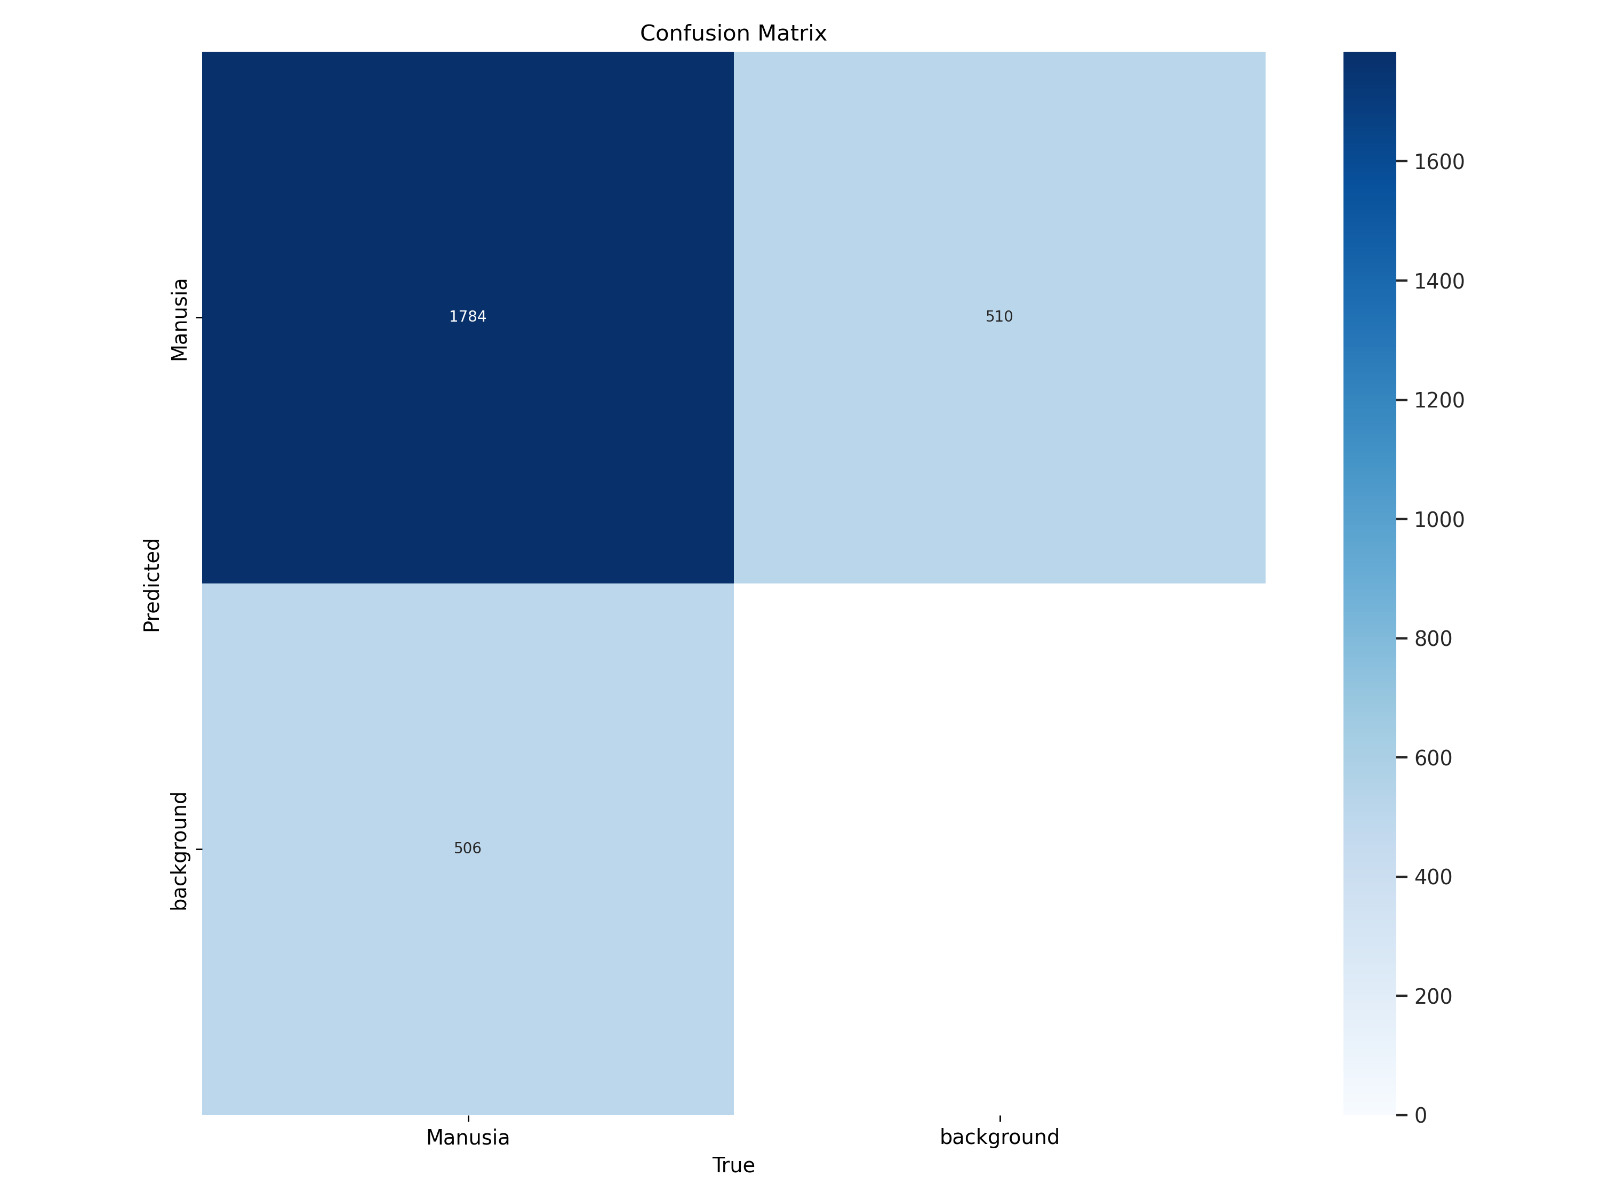
\includegraphics[scale=0.25]{gambar/Confusion matrix yolov11.jpg}
  \caption{\emph{Confusion matrix} pelatihan epoch 150}
  \label{fig:Pengujian Performa}
\end{figure}

Dari gambar 4.5 hasil pelatihan menunjukan dua kelas yakni manusia dan \emph{background}.
Dari hasil tersebut, model berhasil memprediksi hasil benar sebanyak 1784 sampel manusia. 
Namun, terdapat 510 sampel \emph{background} yang salah diklasifikasikan oleh model sebagai manusia. Disisi lain, model melewatkan 
506 sampel manusia yang diklasifikasikan sebagai \emph{background}. Selain itu, tidak ada prediksi yang benar-benar untuk kelas background,
yang mengindikasikan bahwa model cenderung memprioritaskan prediksi kelas manusia dan kurang mampu membedakan objek background dengan baik.
Hal ini menunjukkan adanya kecenderungan false positive dan false negative yang cukup signifikan

\section{Pengujian Performa Model LSTM Menggunakan Confusion Matrix}
Dataset untuk LSTM diambil dalam lima kelas dengan kelas yakni kelas kanan, stop, maju, mundur, dan kiri. Masing-masing kelas berjumlah 30 citra yang
telah di normalisasi tiap citranya, sebagai contoh pada gambar 4.6 merupakan gambar asli atau data mentah.
\begin{figure} [H] \centering
  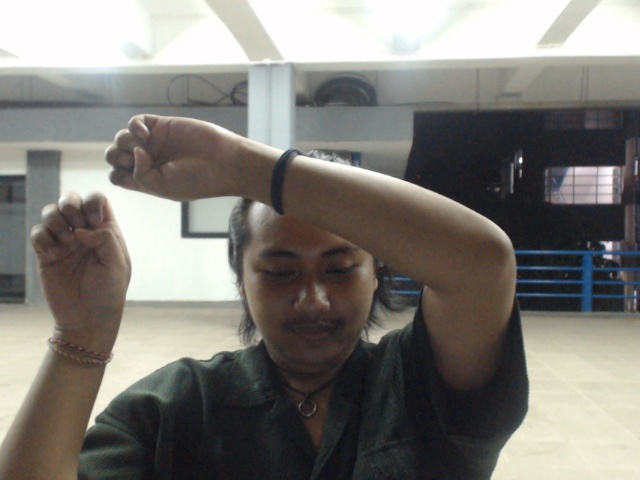
\includegraphics[scale=0.2]{gambar/0-clear.jpg}
  \caption{Dataset kelas kanan \emph{clear}}
  \label{fig:Data set kelas kanan raw}
\end{figure}

Kemudian pada gambar 4.7 menunjukan citra wajah dan tangan dengan titik-titik \emph{landmark} yang telah di deteksi menggunakan media pipe.
\begin{figure} [H] \centering
  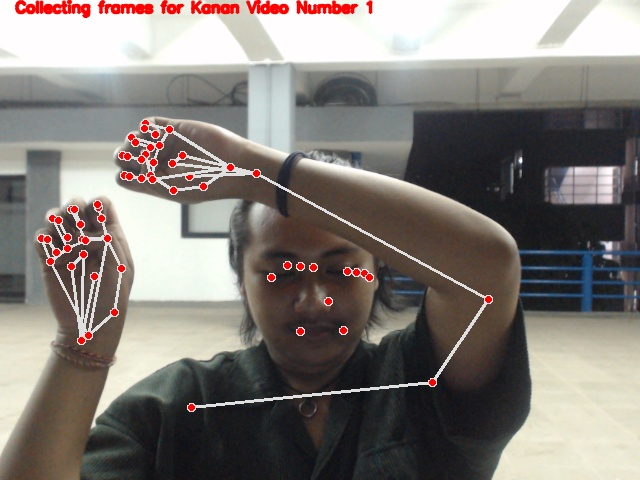
\includegraphics[scale=0.2]{gambar/1.jpg}
  \caption{Dataset kelas kanan \emph{landmark}}
  \label{fig:dataset kelas kanan clear}
\end{figure}
Dari gambar 4.7 diubah kedalam format .npy yang berisi data mentah dari titik-titik \emph{landmark}
yang terdeteksi pada bagian wajah dan dan tangan pada \emph{frame} video. File .npy ini berisi koordinat
2D dari landmark yang citra yang nantinya akan di normalisasi agar koordinat \emph{landmark} menjadi relatif 
terhadap gestur tangan sehingga data menjadi skala yang kosisten dan tidak bergantung pada ukuran asli dari citra. 
Normalisasi ini penting untuk memastikan model LSTM dapat belajar pola gestur tanpa terpengaruh perubahan ukuran citra atau posisi objek.
\begin{table}[htbp]
\centering
\caption{Tabel Sequencial}
\begin{tabular}{|l|l|l|}
\hline
\textbf{Layer (type)} & \textbf{Output Shape} & \textbf{Param \#} \\ \hline
time\_distributed (TimeDistributed) & (None, 30, 128) & 13,952 \\ \hline
lstm (LSTM) & (None, 30, 128) & 131,584 \\ \hline
dropout (Dropout) & (None, 30, 128) & 0 \\ \hline
lstm\_1 (LSTM) & (None, 30, 64) & 49,408 \\ \hline
dropout\_1 (Dropout) & (None, 30, 64) & 0 \\ \hline
lstm\_2 (LSTM) & (None, 32) & 12,416 \\ \hline
dropout\_2 (Dropout) & (None, 32) & 0 \\ \hline
dense\_1 (Dense) & (None, 16) & 528 \\ \hline
dropout\_3 (Dropout) & (None, 16) & 0 \\ \hline
dense\_2 (Dense) & (None, 16) & 272 \\ \hline
dropout\_4 (Dropout) & (None, 16) & 0 \\ \hline
dense\_3 (Dense) & (None, 5) & 85 \\ \hline
\end{tabular}
\end{table}

Tabel 4.1 menunjukkan ringkasan arsitektur model jaringan saraf yang terdiri dari beberapa layer berturut-turut. 
Dimulai dengan layer TimeDistributed yang menghasilkan output berukuran (None, 30, 128) dengan 13.952 parameter, 
yang berfungsi untuk menerapkan layer Dense pada setiap langkah waktu secara independen. Berikutnya terdapat tiga layer LSTM bertingkat, 
masing-masing dengan ukuran output (None, 30, 128), (None, 30, 64), dan (None, 32), serta jumlah parameter yang berkurang 
secara bertahap yaitu 131.584, 49.408, dan 12.416. Layer-layer ini menangani pemrosesan sekuensial data dengan mempertahankan urutan waktu 
dan mengekstrak fitur temporal yang kompleks. Setiap layer LSTM diikuti oleh layer Dropout yang tidak memiliki parameter, berfungsi sebagai 
regularisasi untuk mengurangi overfitting dengan mematikan sebagian neuron secara acak selama pelatihan. Setelah LSTM, model memiliki tiga 
layer Dense berturut-turut dengan ukuran output (None, 16), (None, 16), dan (None, 5) dengan jumlah parameter masing-masing 528, 272, dan 85. 
Layer Dense ini berfungsi untuk memetakan fitur yang telah diekstrak menjadi output klasifikasi akhir dengan 5 kelas, yang ditentukan oleh 
neuron pada layer terakhir.

Berdasarkan hasil akurasi \emph{training} yang telah dilakukan didapatkan bahwa model menghasilkan akurasi validasi bernilai 1 dan akurasi \emph{traininf}
bernilai 0.91. Data ini menunjukan peningkatan akurasi yang cukup baik pada data \emph{training} namun 
pada akurasi validasi mencapai 1.0 beberapa kali yang biasa jarang terjadi pada data validasi yang benar-benar baru dan representatif. Hal ini menandakan
data validasi terlalu kecil  atau kurang sehingga model mudah menghafal. Untuk nilai \emph{loss training} bernilai cukup tinggi di 2.56 dan \emph{loss} validasi di 
di nilai 0.05. Data ini menunjukan nilai \emph{loss training} secara umum menurun dari awal hingga akhir pelatihan, yang berarti model semakin baik dalam 
meminimalkan kesalahan terhadap data \emph{training} seiring dengan berjalannya \emph{epoch}. Untuk \emph{loss} validasi juga menunjukan tren penurunan yang konsisten. 
Hal ini mengindikasikan bahwa model dapat belajar dari data \emph{training} dengan cukup baik. Berikut merupakan grafik dari model akusari dan model \emph{loss} dari pelatihan model LSTM.
\begin{figure} [H] \centering
  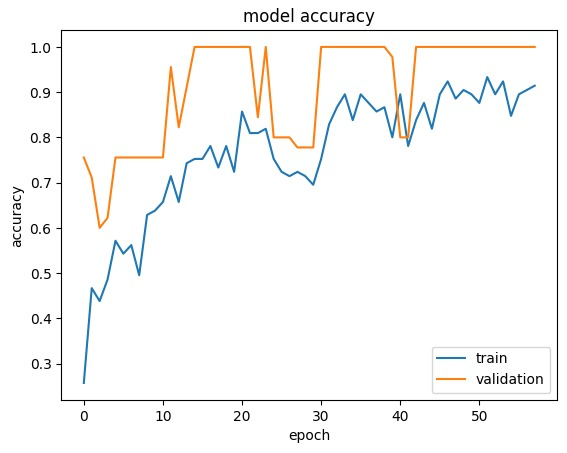
\includegraphics[scale=0.5]{gambar/akurasi model.jpg}
  \caption{Hasil \emph{accuracy} model LSTM}
  \label{fig:Pengujian Performa akurasi lstm}
\end{figure}
\begin{figure} [H] \centering
  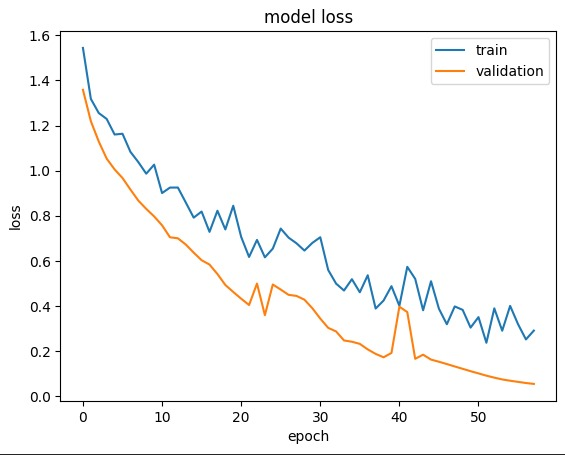
\includegraphics[scale=0.5]{gambar/akurasi loss.jpg}
  \caption{Hasil model \emph{loss} LSTM}
  \label{fig:Pengujian Performa model loss lstm}
\end{figure}

Kemudian berdasarkan model yang telah dilatih, dilakukan pengujian dengan dataset \emph{testing} yang menghasilkan \emph{confusion matrix}.
Gambar 4.10 menunjukkan confusion matrix dari sebuah model klasifikasi dengan lima kelas yaitu Stop, Maju, Mundur, Kanan, dan Kiri. Dari matriks ini dapat dilihat bahwa model mampu
mengklasifikasikan setiap kelas dengan sangat baik tanpa terjadi kesalahan prediksi antar kelas. Misalnya, untuk kelas Stop, seluruh 11 sampel diklasifikasikan dengan benar sebagai Stop, 
dan hal yang sama berlaku untuk kelas Maju dengan 11 sampel yang benar, kelas Mundur dengan 9 sampel, serta kelas Kanan dan Kiri yang masing-masing diklasifikasikan benar sebanyak 7 sampel. 
Tidak terdapat nilai selain diagonal utama yang berarti tidak ada sampel yang salah diklasifikasikan ke kelas lain. Hal ini menunjukkan performa model yang sangat akurat dalam mengenali kelima kelas tersebut. 
\begin{figure} [H] \centering
  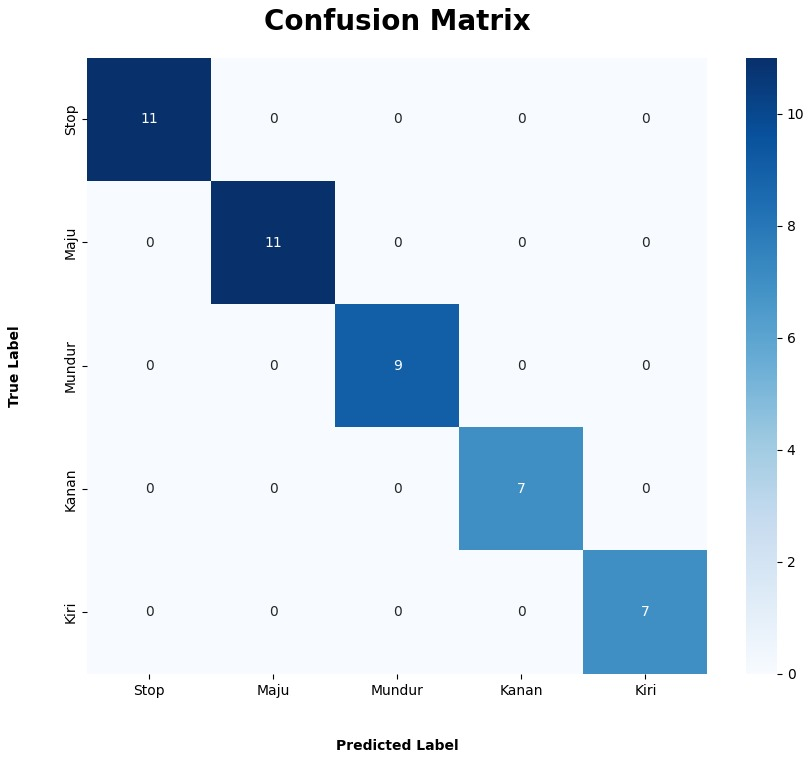
\includegraphics[scale=0.5]{gambar/confusion matrix lstm.jpg}
  \caption{Hasil \emph{confusion matrix} LSTM}
  \label{fig:Grafik confusion matrix lstm}
\end{figure}

\begin{table}[h!]
\centering
\caption{Classification Report}
\begin{tabular}{lcccc}
\hline
\textbf{Class} & \textbf{Precision} & \textbf{Recall} & \textbf{F1-score} & \textbf{Support} \\
\hline
Stop   & 1.00 & 1.00 & 1.00 & 11 \\
Maju   & 1.00 & 1.00 & 1.00 & 11 \\
Mundur & 1.00 & 1.00 & 1.00 & 9  \\
Kanan  & 1.00 & 1.00 & 1.00 & 7  \\
Kiri   & 1.00 & 1.00 & 1.00 & 7  \\
\hline
\textbf{Accuracy}     & \multicolumn{4}{c}{1.00} \\
\textbf{Macro avg}    & 1.00 & 1.00 & 1.00 & 45 \\
\textbf{Weighted avg} & 1.00 & 1.00 & 1.00 & 45 \\
\hline
\end{tabular}
\end{table}

Tabel 4.2 menunjukkan hasil evaluasi model klasifikasi untuk lima kelas, yaitu Stop, Maju, Mundur, Kanan, dan Kiri. Dari tabel tersebut terlihat bahwa model mencapai nilai precision, recall, dan f1-score sebesar 1.00 pada semua kelas, 
yang berarti model mampu mengklasifikasikan setiap kelas dengan sempurna tanpa kesalahan. Support menunjukkan jumlah data uji pada masing-masing kelas, dengan total 45 sampel yang tersebar di kelima kelas tersebut. Nilai accuracy sebesar 1.00 
mengindikasikan bahwa model memiliki akurasi 100\% secara keseluruhan pada data uji ini. Selain itu, nilai macro average dan weighted average yang juga 1.00 memperkuat bahwa performa model sangat baik dan konsisten di seluruh kelas.

\section{Pengujian Berdasarkan FPS}
Pengujian FPS akan dilakukan pada dua device yang pertama adalah pengujian pada device Laptop, dan pengujian pada device NUC. Dalam pengujian ini akan diambil nilai FPS sebanyak 30 kali yang sesuai dengan output sistem dan sudah diolah pada bagian sebelumnya.

Pada pengujian ini akan diambil nilai FPS pada laptop dan FPS pada NUC. Spesifikasi laptop yang digunakan untuk pengujian ini pada tabel  :

\begin{longtable}{|c|c|}
  \caption{Spesifikasi Laptop}
  \label{tb:Spesifikasi Laptop}                                   \\
  \hline
  \rowcolor[HTML]{C0C0C0}
  \textbf{Komponen} & \textbf{Spesifikasi}  \\
  \hline
  CPU            & Intel(R) Core(TM) i5-10300H CPU @2.50GHz(8CPU)        \\ \hline
  RAM            & 16 GB DDR4-2666 SDRAM        \\ \hline
  GPU            & NVIDIA® GeForce RTX™ 2060 with Max-Q design           \\ \hline
  \hline
\end{longtable}

Spesifikasi NUC yang digunakan untuk pengujian ini pada tabel  :

\begin{longtable}{|c|c|}
    \caption{Spesifikasi NUC}
    \label{tb:Spesifikasi NUC}                             \\
    \hline   
    \rowcolor[HTML]{C0C0C0}
    \textbf{Komponen} & \textbf{Spesifikasi} \\
    \hline
  CPU            &  Intel® Core™ i7-1165G7        \\
  RAM            & 32 GBLPDDR4        \\
  OS            & Windows 11 Home Single Language           \\
  \hline
\end{longtable}

Baik system kontrol maupun system pengereman otomatis akan diambil nilai fpsnya, selain itu setiap jenis arsitektur YOLO juga akan dibandingkan untuk menilai efisiensi sistem berdasarkan jenis arsitektur YOLO yang digunakan. Pengujian ini dilakukan dengan cara menjalankan sistem pada laptop dan NUC, kemudian merekam hasil dari pengujian tersebut. Hasil dari pengujian ini akan ditampilkan dalam bentuk tabel.

\newpage

\subsection{Pengujian Model YOLOv11 Berdasarkan FPS pada Laptop}

Pengujian dilakukan pada laptop dengan spesifikasi yang telah disebutkan sebelumnya. Pengujian ini dilakukan dengan cara menjalankan sistem pada laptop dan merekam hasil dari pengujian tersebut. Hasil dari pengujian ini akan ditampilkan dalam bentuk tabel. Gambar \ref{fig:Foto pengujian fps laptop} merupakan gambar pengambilan data fps pada laptop.

\begin{figure} [H] \centering
  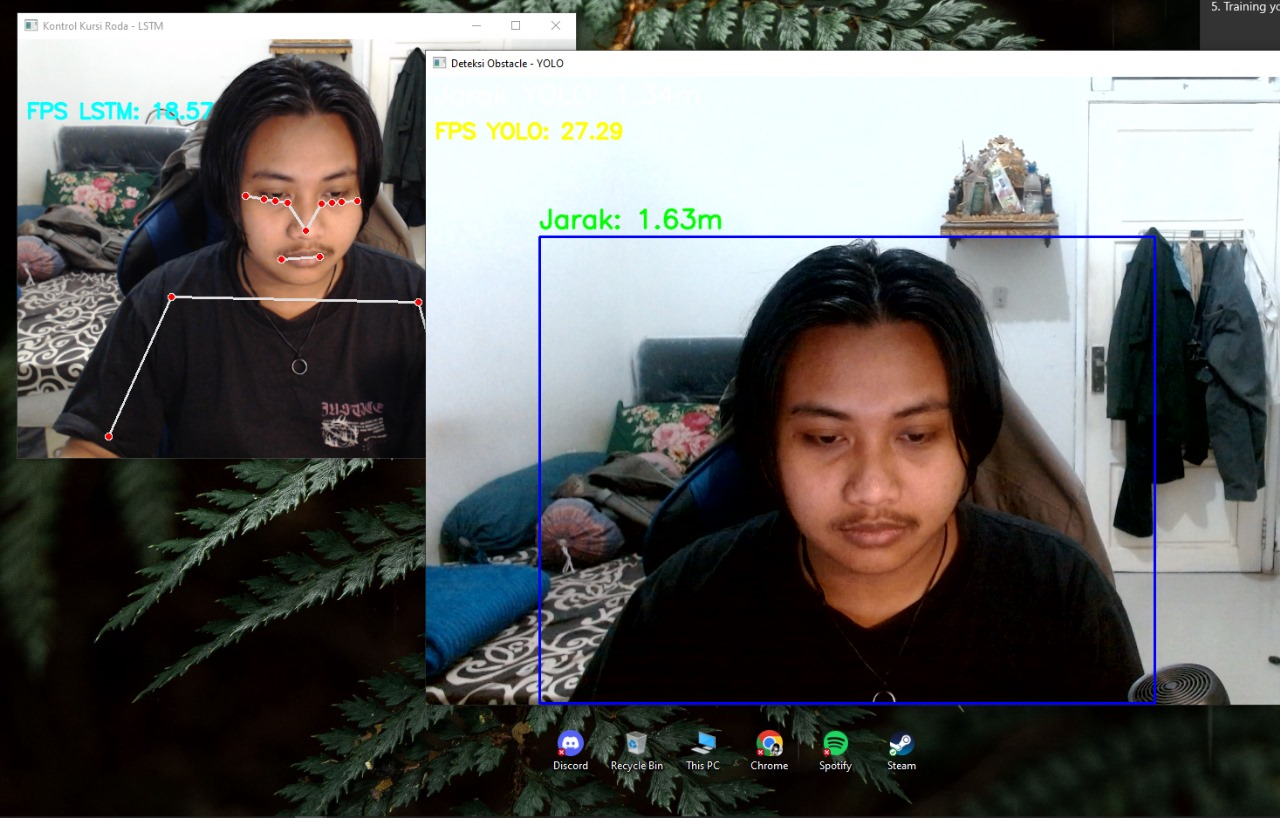
\includegraphics[scale=0.3]{gambar/devafps.jpg}
  \caption{Pengujian FPS pada Laptop}
  \label{fig:Foto pengujian fps laptop}
\end{figure}

Pada tabel \ref{tb:TabelYoloLaptop} merupakan hasil dari pengujian model YOLOv11 berdasarkan FPS pada Laptop. Dari hasil tersebut didapatkan rata rata FPS sebesar 24,969 , dengan nilai tertinggi FPS sebesar 35,81 dan nilai terendah sebesar 12,8.

\begin{table}[H]
  \caption{Nilai Pengujian Model YOLOv11 Berdasarkan FPS pada Laptop} 
  \label{tb:TabelYolov11Laptop}
  \centering
  \begin{tabular}{|l|l|l|l|l|l|l|l|}
  \cline{1-2} \cline{4-5} \cline{7-8}
  No & FPS   &  & No & FPS   &  & No & FPS   \\ \cline{1-2} \cline{4-5} \cline{7-8} 
  1  & 21,8  &  & 11 & 21,82 &  & 21 & 23,32 \\ \cline{1-2} \cline{4-5} \cline{7-8} 
  2  & 20,89 &  & 12 & 20,89 &  & 22 & 23,89 \\ \cline{1-2} \cline{4-5} \cline{7-8} 
  3  & 25,7  &  & 13 & 17,9  &  & 23 & 21,18 \\ \cline{1-2} \cline{4-5} \cline{7-8} 
  4  & 12,8  &  & 14 & 23,57 &  & 24 & 31,33 \\ \cline{1-2} \cline{4-5} \cline{7-8} 
  5  & 23,32 &  & 15 & 21,77 &  & 25 & 30,38 \\ \cline{1-2} \cline{4-5} \cline{7-8} 
  6  & 34,57 &  & 16 & 17,34 &  & 26 & 29,49 \\ \cline{1-2} \cline{4-5} \cline{7-8} 
  7  & 21,33 &  & 17 & 26,39 &  & 27 & 33,42 \\ \cline{1-2} \cline{4-5} \cline{7-8} 
  8  & 35,81 &  & 18 & 19,28 &  & 28 & 32,34 \\ \cline{1-2} \cline{4-5} \cline{7-8} 
  9  & 21,8  &  & 19 & 32,34 &  & 29 & 28,31 \\ \cline{1-2} \cline{4-5} \cline{7-8} 
  10 & 24,45 &  & 20 & 29,54 &  & 30 & 22,12 \\ \cline{1-2} \cline{4-5} \cline{7-8} 
  \end{tabular}
  \end{table}

Pada pengujian menggunakan model YOLOv11 pada laptop ini, hasil yang didapatkan sangat baik dimana FPS menyentuh angka yang cukup tinggi. Hal ini menunjukan bahwa sistem dapat berjalan dengan baik dan efisien, hal ini akan menjadi sangat penting bahwa output dari model YOLOv11 akan menjadi variabel utama dalam sistem pengereman otomatis.

\subsection{Pengujian Model YOLOv8 Berdasarkan FPS pada Laptop}

Pengujian dilakukan pada laptop dengan spesifikasi yang telah disebutkan sebelumnya. Pengujian ini dilakukan dengan cara menjalankan sistem pada laptop dan merekam hasil dari pengujian tersebut. Hasil dari pengujian ini akan ditampilkan dalam bentuk tabel. Gambar \ref{fig:Foto pengujian fps laptop} merupakan gambar pengambilan data fps pada laptop.

Pada tabel \ref{tb:TabelYoloLaptop} merupakan hasil dari pengujian model YOLOv8 berdasarkan FPS pada Laptop. Dari hasil tersebut didapatkan rata rata FPS sebesar 27.xxx, dengan nilai tertinggi FPS sebesar 30.xxx dan nilai terendah sebesar 19.xxx.

\begin{table}[H]
  \caption{Nilai Pengujian Model YOLOv8 Berdasarkan FPS pada Laptop} 
  \label{tb:TabelYolov8Laptop}
  \centering
  \begin{tabular}{|l|l|l|l|l|l|l|l|}
  \cline{1-2} \cline{4-5} \cline{7-8}
  No & FPS  &  & No & FPS  &  & No & FPS  \\ \cline{1-2} \cline{4-5} \cline{7-8} 
  1  & 6,68 &  & 11 & 6,24 &  & 21 & 5,12 \\ \cline{1-2} \cline{4-5} \cline{7-8} 
  2  & 7,43 &  & 12 & 4,77 &  & 22 & 8,43 \\ \cline{1-2} \cline{4-5} \cline{7-8} 
  3  & 6,68 &  & 13 & 7,43 &  & 23 & 6,73 \\ \cline{1-2} \cline{4-5} \cline{7-8} 
  4  & 8,89 &  & 14 & 8,36 &  & 24 & 8,36 \\ \cline{1-2} \cline{4-5} \cline{7-8} 
  5  & 6,08 &  & 15 & 6,68 &  & 25 & 6,43 \\ \cline{1-2} \cline{4-5} \cline{7-8} 
  6  & 7,43 &  & 16 & 7,23 &  & 26 & 5,33 \\ \cline{1-2} \cline{4-5} \cline{7-8} 
  7  & 8,36 &  & 17 & 4,12 &  & 27 & 6,59 \\ \cline{1-2} \cline{4-5} \cline{7-8} 
  8  & 5,12 &  & 18 & 6,88 &  & 28 & 7,1  \\ \cline{1-2} \cline{4-5} \cline{7-8} 
  9  & 6,14 &  & 19 & 7,48 &  & 29 & 5,43 \\ \cline{1-2} \cline{4-5} \cline{7-8} 
  10 & 7,87 &  & 20 & 7,42 &  & 30 & 6,65 \\ \cline{1-2} \cline{4-5} \cline{7-8} 
  \end{tabular}
  \end{table}

Pada pengujian menggunakan model YOLOv8 pada laptop ini, hasil yang didapatkan sangat baik dimana FPS menyentuh angka yang cukup tinggi. Hal ini menunjukan bahwa sistem dapat berjalan dengan baik dan efisien, hal ini akan menjadi sangat penting bahwa output dari model YOLOv8 akan menjadi variabel utama dalam sistem pengereman otomatis.

\subsection{Pengujian Model YOLOv12 Berdasarkan FPS pada Laptop}

Pengujian dilakukan pada laptop dengan spesifikasi yang telah disebutkan sebelumnya. Pengujian ini dilakukan dengan cara menjalankan sistem pada laptop dan merekam hasil dari pengujian tersebut. Hasil dari pengujian ini akan ditampilkan dalam bentuk tabel. Gambar \ref{fig:Foto pengujian fps laptop} merupakan gambar pengambilan data fps pada laptop.

Pada tabel \ref{tb:TabelYoloLaptop} merupakan hasil dari pengujian model YOLOv8 berdasarkan FPS pada Laptop. Dari hasil tersebut didapatkan rata rata FPS sebesar 27.xxx, dengan nilai tertinggi FPS sebesar 30.xxx dan nilai terendah sebesar 19.xxx.

\begin{table}[H]
  \centering
  \caption{Nilai Pengujian Model YOLOv12 Berdasarkan FPS pada Laptop} 
  \label{tb:TabelYolov12xLaptop}
  \begin{tabular}{|l|l|l|l|l|l|l|l|}
  \cline{1-2} \cline{4-5} \cline{7-8}
  No & FPS &  & No & FPS &  & No & FPS \\ \cline{1-2} \cline{4-5} \cline{7-8} 
  1  &     &  & 11 &     &  & 21 &     \\ \cline{1-2} \cline{4-5} \cline{7-8} 
  2  &     &  & 12 &     &  & 22 &     \\ \cline{1-2} \cline{4-5} \cline{7-8} 
  3  &     &  & 13 &     &  & 23 &     \\ \cline{1-2} \cline{4-5} \cline{7-8} 
  4  &     &  & 14 &     &  & 24 &     \\ \cline{1-2} \cline{4-5} \cline{7-8} 
  5  &     &  & 15 &     &  & 25 &     \\ \cline{1-2} \cline{4-5} \cline{7-8} 
  6  &     &  & 16 &     &  & 26 &     \\ \cline{1-2} \cline{4-5} \cline{7-8} 
  7  &     &  & 17 &     &  & 27 &     \\ \cline{1-2} \cline{4-5} \cline{7-8} 
  8  &     &  & 18 &     &  & 28 &     \\ \cline{1-2} \cline{4-5} \cline{7-8} 
  9  &     &  & 19 &     &  & 29 &     \\ \cline{1-2} \cline{4-5} \cline{7-8} 
  10 &     &  & 20 &     &  & 30 &     \\ \cline{1-2} \cline{4-5} \cline{7-8} 
  \end{tabular}
  \end{table}

Pada pengujian menggunakan model YOLOv12 pada laptop ini, hasil yang didapatkan sangat baik dimana FPS menyentuh angka yang cukup tinggi. Hal ini menunjukan bahwa sistem dapat berjalan dengan baik dan efisien, hal ini akan menjadi sangat penting bahwa output dari model YOLOv12 akan menjadi variabel utama dalam sistem pengereman otomatis.

\subsection{Pengujian Model LSTM Berdasarkan FPS pada Laptop}

Pengujian dilakukan pada laptop dengan spesifikasi yang telah disebutkan sebelumnya. Pengujian ini dilakukan dengan cara menjalankan sistem pada laptop dan merekam hasil dari pengujian tersebut. Hasil dari pengujian ini akan ditampilkan dalam bentuk tabel. Gambar \ref{fig:Foto pengujian fps laptop} merupakan gambar pengambilan data fps pada laptop.

Pada tabel \ref{tb:TabelYoloLaptop} merupakan hasil dari pengujian model LSTM berdasarkan FPS pada Laptop. Dari hasil tersebut didapatkan rata rata FPS sebesar 27.xxx, dengan nilai tertinggi FPS sebesar 30.xxx dan nilai terendah sebesar 19.xxx.


\begin{table}[H]
  \centering
  \caption{Nilai Pengujian Model LSTM Berdasarkan FPS pada Laptop} 
  \label{tb:TabelLSTMLaptop}
  \begin{tabular}{|l|l|l|l|l|l|l|l|}
  \cline{1-2} \cline{4-5} \cline{7-8}
  No & FPS   &  & No & FPS   &  & No & FPS   \\ \cline{1-2} \cline{4-5} \cline{7-8} 
  1  & 25,91 &  & 11 & 23,09 &  & 21 & 22,38 \\ \cline{1-2} \cline{4-5} \cline{7-8} 
  2  & 22,43 &  & 12 & 24,67 &  & 22 & 22,79 \\ \cline{1-2} \cline{4-5} \cline{7-8} 
  3  & 23,25 &  & 13 & 22,76 &  & 23 & 24,57 \\ \cline{1-2} \cline{4-5} \cline{7-8} 
  4  & 23,98 &  & 14 & 25,74 &  & 24 & 22,73 \\ \cline{1-2} \cline{4-5} \cline{7-8} 
  5  & 26,32 &  & 15 & 23,46 &  & 25 & 22,62 \\ \cline{1-2} \cline{4-5} \cline{7-8} 
  6  & 22,19 &  & 16 & 25,3  &  & 26 & 25,03 \\ \cline{1-2} \cline{4-5} \cline{7-8} 
  7  & 23,32 &  & 17 & 25,96 &  & 27 & 23,17 \\ \cline{1-2} \cline{4-5} \cline{7-8} 
  8  & 22,57 &  & 18 & 22,51 &  & 28 & 25,16 \\ \cline{1-2} \cline{4-5} \cline{7-8} 
  9  & 22,76 &  & 19 & 24,97 &  & 29 & 25,06 \\ \cline{1-2} \cline{4-5} \cline{7-8} 
  10 & 24,78 &  & 20 & 22,43 &  & 30 & 22,48 \\ \cline{1-2} \cline{4-5} \cline{7-8} 
  \end{tabular}
\end{table}

Pada pengujian menggunakan model LSTM pada laptop ini, hasil yang didapatkan sangat baik dimana FPS menyentuh angka yang cukup tinggi. Hal ini menunjukan bahwa sistem dapat berjalan dengan baik dan efisien, hal ini akan menjadi sangat penting bahwa output klasifikasi gestur dari model LSTM akan digunakan dalam sistem kendali kursi roda.


\subsection{Pengujian Model YOLOv11 Berdasarkan FPS pada NUC}

Pengujian dilakukan pada NUC dengan spesifikasi yang telah disebutkan sebelumnya. Pengujian ini dilakukan dengan cara menjalankan sistem pada NUC dan merekam hasil dari pengujian tersebut. Hasil dari pengujian ini akan ditampilkan dalam bentuk tabel. Gambar \ref{fig:Foto pengujian fps NUC} merupakan gambar pengambilan data fps pada laptop.

\begin{figure} [H] \centering
  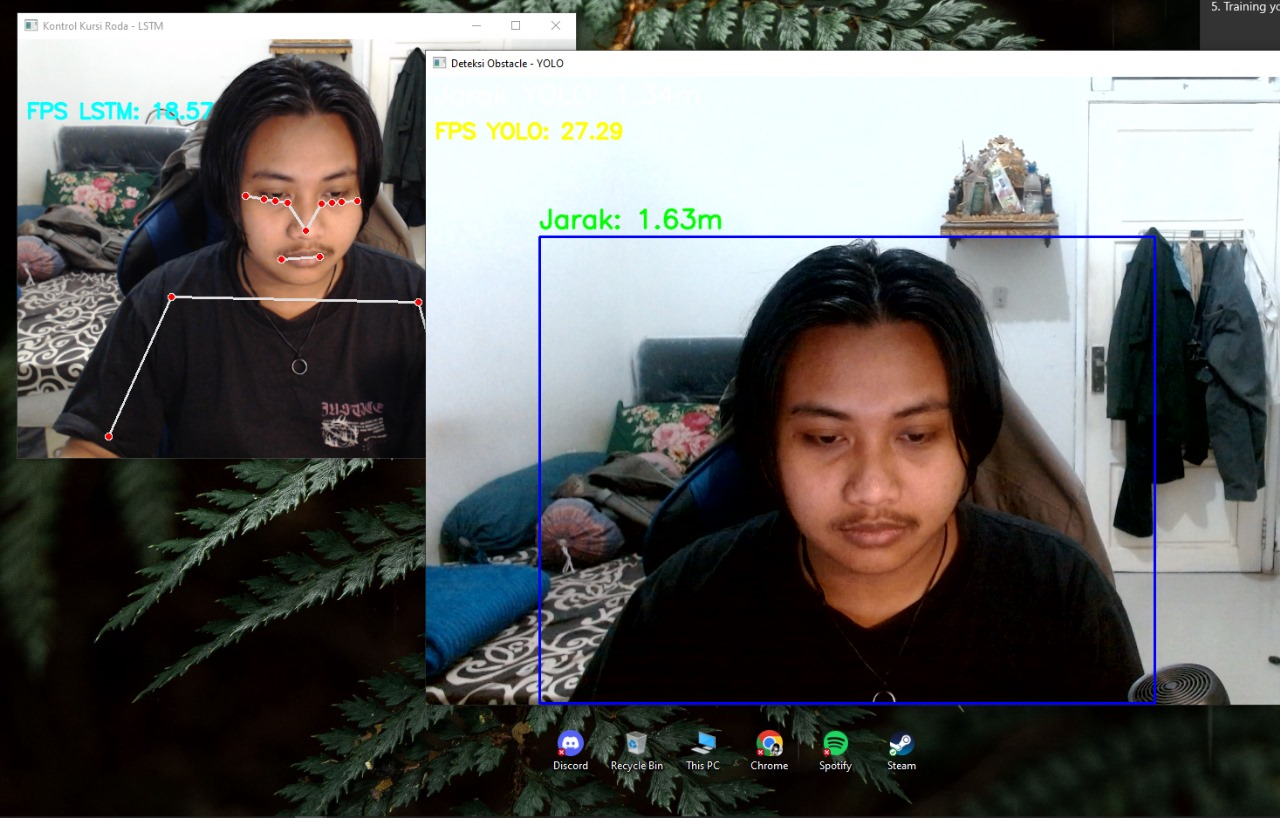
\includegraphics[scale=0.3]{gambar/devafps.jpg}
  \caption{Pengujian FPS pada NUC}
  \label{fig:Foto pengujian fps NUC}
\end{figure}

Pada tabel \ref{tb:TabelYoloLaptop} merupakan hasil dari pengujian model YOLOv11 berdasarkan FPS pada Laptop. Dari hasil tersebut didapatkan rata rata FPS sebesar 27.xxx, dengan nilai tertinggi FPS sebesar 30.xxx dan nilai terendah sebesar 19.xxx.

\begin{table}[H]
  \caption{Nilai Pengujian Model YOLOv11 Berdasarkan FPS pada NUC} 
  \label{tb:TabelYolov11NUC}
  \centering
  \begin{tabular}{|l|l|l|l|l|l|l|l|}
  \cline{1-2} \cline{4-5} \cline{7-8}
  No & FPS   &  & No & FPS   &  & No & FPS   \\ \cline{1-2} \cline{4-5} \cline{7-8} 
  1  & 9,12  &  & 11 & 10,4  &  & 21 & 9,59  \\ \cline{1-2} \cline{4-5} \cline{7-8} 
  2  & 10,02 &  & 12 & 11,21 &  & 22 & 9,97  \\ \cline{1-2} \cline{4-5} \cline{7-8} 
  3  & 10    &  & 13 & 10,87 &  & 23 & 10,09 \\ \cline{1-2} \cline{4-5} \cline{7-8} 
  4  & 9,94  &  & 14 & 9,87  &  & 24 & 9,97  \\ \cline{1-2} \cline{4-5} \cline{7-8} 
  5  & 10,28 &  & 15 & 9,23  &  & 25 & 10,21 \\ \cline{1-2} \cline{4-5} \cline{7-8} 
  6  & 9,54  &  & 16 & 10,65 &  & 26 & 9,89  \\ \cline{1-2} \cline{4-5} \cline{7-8} 
  7  & 9,95  &  & 17 & 10,02 &  & 27 & 10    \\ \cline{1-2} \cline{4-5} \cline{7-8} 
  8  & 9,86  &  & 18 & 9,92  &  & 28 & 10,19 \\ \cline{1-2} \cline{4-5} \cline{7-8} 
  9  & 10,32 &  & 19 & 10,03 &  & 29 & 10,22 \\ \cline{1-2} \cline{4-5} \cline{7-8} 
  10 & 9,94  &  & 20 & 10,09 &  & 30 & 9,87  \\ \cline{1-2} \cline{4-5} \cline{7-8} 
  \end{tabular}
\end{table}
Pada pengujian menggunakan model YOLOv11 pada laptop ini, hasil yang didapatkan sangat baik dimana FPS menyentuh angka yang cukup tinggi. Hal ini menunjukan bahwa sistem dapat berjalan dengan baik dan efisien, hal ini akan menjadi sangat penting bahwa output dari model YOLOv11 akan menjadi variabel utama dalam sistem pengereman otomatis.

\subsection{Pengujian Model YOLOv8 Berdasarkan FPS pada NUC}

Pengujian dilakukan pada laptop dengan spesifikasi yang telah disebutkan sebelumnya. Pengujian ini dilakukan dengan cara menjalankan sistem pada laptop dan merekam hasil dari pengujian tersebut. Hasil dari pengujian ini akan ditampilkan dalam bentuk tabel. Gambar \ref{fig:Foto pengujian fps laptop} merupakan gambar pengambilan data fps pada laptop.

Pada tabel \ref{tb:TabelYoloLaptop} merupakan hasil dari pengujian model YOLOv8 berdasarkan FPS pada Laptop. Dari hasil tersebut didapatkan rata rata FPS sebesar 27.xxx, dengan nilai tertinggi FPS sebesar 30.xxx dan nilai terendah sebesar 19.xxx.

\begin{table}[H]
  \caption{Nilai Pengujian Model YOLOv8 Berdasarkan FPS pada NUC} 
  \label{tb:TabelYolov8NUC}
  \centering
  \begin{tabular}{|l|l|l|l|l|l|l|l|}
  \cline{1-2} \cline{4-5} \cline{7-8}
  No & FPS  &  & No & FPS  &  & No & FPS  \\ \cline{1-2} \cline{4-5} \cline{7-8} 
  1  & 5,43 &  & 11 & 6,34 &  & 21 & 5,32 \\ \cline{1-2} \cline{4-5} \cline{7-8} 
  2  & 3,65 &  & 12 & 5,76 &  & 22 & 6,43 \\ \cline{1-2} \cline{4-5} \cline{7-8} 
  3  & 5,67 &  & 13 & 5,98 &  & 23 & 5,65 \\ \cline{1-2} \cline{4-5} \cline{7-8} 
  4  & 6,54 &  & 14 & 5,34 &  & 24 & 6,19 \\ \cline{1-2} \cline{4-5} \cline{7-8} 
  5  & 5,34 &  & 15 & 6,32 &  & 25 & 5,71 \\ \cline{1-2} \cline{4-5} \cline{7-8} 
  6  & 4,98 &  & 16 & 4,94 &  & 26 & 4,31 \\ \cline{1-2} \cline{4-5} \cline{7-8} 
  7  & 5,74 &  & 17 & 5,53 &  & 27 & 4,67 \\ \cline{1-2} \cline{4-5} \cline{7-8} 
  8  & 5,01 &  & 18 & 5,67 &  & 28 & 5,43 \\ \cline{1-2} \cline{4-5} \cline{7-8} 
  9  & 6,43 &  & 19 & 6,32 &  & 29 & 4,81 \\ \cline{1-2} \cline{4-5} \cline{7-8} 
  10 & 7,33 &  & 20 & 5,12 &  & 30 & 6,53 \\ \cline{1-2} \cline{4-5} \cline{7-8} 
  \end{tabular}
\end{table}

Pada pengujian menggunakan model YOLOv8 pada laptop ini, hasil yang didapatkan sangat baik dimana FPS menyentuh angka yang cukup tinggi. Hal ini menunjukan bahwa sistem dapat berjalan dengan baik dan efisien, hal ini akan menjadi sangat penting bahwa output dari model YOLOv8 akan menjadi variabel utama dalam sistem pengereman otomatis.

\subsection{Pengujian Model YOLOv12 Berdasarkan FPS pada NUC}

Pengujian dilakukan pada laptop dengan spesifikasi yang telah disebutkan sebelumnya. Pengujian ini dilakukan dengan cara menjalankan sistem pada laptop dan merekam hasil dari pengujian tersebut. Hasil dari pengujian ini akan ditampilkan dalam bentuk tabel. Gambar \ref{fig:Foto pengujian fps laptop} merupakan gambar pengambilan data fps pada laptop.

Pada tabel \ref{tb:TabelYoloLaptop} merupakan hasil dari pengujian model YOLOv8 berdasarkan FPS pada Laptop. Dari hasil tersebut didapatkan rata rata FPS sebesar 27.xxx, dengan nilai tertinggi FPS sebesar 30.xxx dan nilai terendah sebesar 19.xxx.

\begin{table}[H]
  \centering
  \caption{Nilai Pengujian Model YOLOv12 Berdasarkan FPS pada NUC} 
  \label{tb:TabelYolov12Nuc}
  \begin{tabular}{|l|l|l|l|l|l|l|l|}
  \cline{1-2} \cline{4-5} \cline{7-8}
  No & FPS &  & No & FPS &  & No & FPS \\ \cline{1-2} \cline{4-5} \cline{7-8} 
  1  &     &  & 11 &     &  & 21 &     \\ \cline{1-2} \cline{4-5} \cline{7-8} 
  2  &     &  & 12 &     &  & 22 &     \\ \cline{1-2} \cline{4-5} \cline{7-8} 
  3  &     &  & 13 &     &  & 23 &     \\ \cline{1-2} \cline{4-5} \cline{7-8} 
  4  &     &  & 14 &     &  & 24 &     \\ \cline{1-2} \cline{4-5} \cline{7-8} 
  5  &     &  & 15 &     &  & 25 &     \\ \cline{1-2} \cline{4-5} \cline{7-8} 
  6  &     &  & 16 &     &  & 26 &     \\ \cline{1-2} \cline{4-5} \cline{7-8} 
  7  &     &  & 17 &     &  & 27 &     \\ \cline{1-2} \cline{4-5} \cline{7-8} 
  8  &     &  & 18 &     &  & 28 &     \\ \cline{1-2} \cline{4-5} \cline{7-8} 
  9  &     &  & 19 &     &  & 29 &     \\ \cline{1-2} \cline{4-5} \cline{7-8} 
  10 &     &  & 20 &     &  & 30 &     \\ \cline{1-2} \cline{4-5} \cline{7-8} 
  \end{tabular}
\end{table}

Pada pengujian menggunakan model YOLOv12 pada laptop ini, hasil yang didapatkan sangat baik dimana FPS menyentuh angka yang cukup tinggi. Hal ini menunjukan bahwa sistem dapat berjalan dengan baik dan efisien, hal ini akan menjadi sangat penting bahwa output dari model YOLOv12 akan menjadi variabel utama dalam sistem pengereman otomatis.

\subsection{Pengujian Model LSTM Berdasarkan FPS pada NUC}

Pengujian dilakukan pada laptop dengan spesifikasi yang telah disebutkan sebelumnya. Pengujian ini dilakukan dengan cara menjalankan sistem pada laptop dan merekam hasil dari pengujian tersebut. Hasil dari pengujian ini akan ditampilkan dalam bentuk tabel. Gambar \ref{fig:Foto pengujian fps laptop} merupakan gambar pengambilan data fps pada laptop.

Pada tabel \ref{tb:TabelYoloLaptop} merupakan hasil dari pengujian model LSTM berdasarkan FPS pada Laptop. Dari hasil tersebut didapatkan rata rata FPS sebesar 27.xxx, dengan nilai tertinggi FPS sebesar 30.xxx dan nilai terendah sebesar 19.xxx. 


\begin{table}[H]
  \centering
  \caption{Nilai Pengujian Model LSTM Berdasarkan FPS pada Laptop} 
  \label{tb:TabelLSTMLaptop}
  \begin{tabular}{|l|l|l|l|l|l|l|l|}
  \cline{1-2} \cline{4-5} \cline{7-8}
  No & FPS   &  & No & FPS   &  & No & FPS   \\ \cline{1-2} \cline{4-5} \cline{7-8} 
  1  & 14,32 &  & 11 & 12,32 &  & 21 & 16,44 \\ \cline{1-2} \cline{4-5} \cline{7-8} 
  2  & 12,34 &  & 12 & 11,43 &  & 22 & 16,71 \\ \cline{1-2} \cline{4-5} \cline{7-8} 
  3  & 14,03 &  & 13 & 12,54 &  & 23 & 14,86 \\ \cline{1-2} \cline{4-5} \cline{7-8} 
  4  & 12,39 &  & 14 & 12,87 &  & 24 & 13,32 \\ \cline{1-2} \cline{4-5} \cline{7-8} 
  5  & 14,71 &  & 15 & 13,74 &  & 25 & 12,86 \\ \cline{1-2} \cline{4-5} \cline{7-8} 
  6  & 13,22 &  & 16 & 13,93 &  & 26 & 15,92 \\ \cline{1-2} \cline{4-5} \cline{7-8} 
  7  & 12,19 &  & 17 & 15,92 &  & 27 & 16,71 \\ \cline{1-2} \cline{4-5} \cline{7-8} 
  8  & 12,89 &  & 18 & 12,43 &  & 28 & 13,43 \\ \cline{1-2} \cline{4-5} \cline{7-8} 
  9  & 14,42 &  & 19 & 15,92 &  & 29 & 12,43 \\ \cline{1-2} \cline{4-5} \cline{7-8} 
  10 & 12,42 &  & 20 & 12,86 &  & 30 & 11,56 \\ \cline{1-2} \cline{4-5} \cline{7-8} 
  \end{tabular}
  \end{table}

Pada pengujian menggunakan model LSTM pada laptop ini, hasil yang didapatkan sangat baik dimana FPS menyentuh angka yang cukup tinggi. Hal ini menunjukan bahwa sistem dapat berjalan dengan baik dan efisien, hal ini akan menjadi sangat penting bahwa output klasifikasi gestur dari model LSTM akan digunakan dalam sistem kendali kursi roda.

\newpage
\section{Pengujian berdasarkan hasil respond time}
Pengujian respond time dilakukan dengan cara mencatat hasil klasifikasi dari model LSTM dan hasil deteksi objek dari Model. Output dari model tersebut sudah dilengkapi dengan Arah dan timestamp yang dihasilkan untuk model klasifikasi gestur, dan timestamp pengereman yang dihasilkan untuk model deteksi objek. Dimana timestamp tersebut dibandingkan hasil pengiriman dari sistem dan hasil penerimaan dari hardware, dimana kedua data tersebut diambil melalui Terminal Visual Studio dan Arduino IDE. Berikut merupakan contoh data mentah untuk kedua hasil output: 

\begin{lstlisting}[language=c]
  
  0: 480x800 1 Manusia, 101.8ms
  Speed: 12.5ms preprocess, 101.8ms inference, 1.2ms postprocess per image at shape (1, 3, 480, 800)
  [LSTM]  Mundur (D) == 04:06:10.098
  Aksi: Mundur

  0: 480x800 2 Manusias, 95.5ms
  Speed: 16.2ms preprocess, 95.5ms inference, 1.3ms postprocess per image at shape (1, 3, 480, 800)
  [LSTM]  Stop (C) == 04:06:10.426
  Aksi: Stop

  0: 480x800 2 Manusias, 95.5ms
  Speed: 3.9ms preprocess, 74.0ms inference, 1.3ms postprocess per image at shape (1, 3, 480, 800)
  [LSTM]  Maju (B) == 04:06:10.554
  Aksi: Maju

\end{lstlisting}

Data diatas merupakan sampel data mentah yang didapatkan dari hasil klasifikasi gesture menggunakan model LSTM. Adapun output untuk model YOLO dipisahkan penulisannya dari hasil klasifikasi gesture, hal ini bertujuan untuk mempermudah dalam pengolahan data. Berikut merupakan contoh data mentah untuk hasil deteksi objek menggunakan model YOLOv11, YOLOv8 dan YOLOv12:

\begin{lstlisting}[language=c]
  
  0: 480x800 1 Manusia, 81.6ms
  Speed: 10.0ms preprocess, 81.6ms inference, 1.3ms postprocess per image at shape (1, 3, 480, 800)
  STOP
  [YOLO] BREAK Response ======== 04:06:10.553
  
  0: 480x800 1 Manusia, 73.0ms
  Speed: 5.5ms preprocess, 73.0ms inference, 1.4ms postprocess per image at shape (1, 3, 480, 800)
  STOP 
  [YOLO] BREAK Response ======== 04:06:10.737

\end{lstlisting}

\newpage
Output yang didapatkan pada ardruino berisikan Timestamp. Timestamp yang dihasilkan yaitu \emph{Timestamp Receive ESP} dan \emph{Timestamp Receive Motor}. contoh outputnya dapat dilihat sebagai berikut.

\begin{lstlisting}[language=python]
  BELOK KANAN,0.8,2024-05-08 22:18:14.263
  MAJU,0.4,2024-05-08 22:18:18.762
  BELOK KANAN,0.0,2024-05-08 22:18:28.614
  MAJU,0.0,2024-05-08 22:18:30.940
  BELOK KANAN,1.2,2024-05-08 22:18:32.899
  MAJU,0.8,2024-05-08 22:18:34.728
  BELOK KANAN,0.0,2024-05-08 22:18:36.392
\end{lstlisting}

Pengujian ini akan dihitung response time sejumlah 30 kali yang akan dijabarkan pada tabel refxxxxx Hasil rsponse time akan diuji untuk mendapatkan waktu yang dibutuhkan untuk melakukan pendeteksian maupun klasifikasi gesture pada model yang kemudian diteruskan ke ESP32 hingga ke motor kursi roda mulai bergerak. Pengujian ini dilakukan secara real time pada perangkat Laptop, perhitungan delay didapatkan dari mulai dikirim hingga berhentinya motor pada kursi roda. Mengingat bahwa baik inference maupun response kirim dari kedua model berbeda maka tabel akan dibedakan menjadi dua tabel, yaitu tabel untuk model YOLO dan tabel untuk model LSTM.

\begin{table}[H]
  \centering
  \label{tb:TabelHasilPengujianResponseTimeLSTM}
  \caption{Hasil Pengujian Response Time Model LSTM}
  \begin{tabular}{|l|l|l|l|l|l|}
  \hline
  Inference & Sent & Receive & Motor & Delay & Arah \\ \hline
            &      &         &       &       &      \\ \hline
            &      &         &       &       &      \\ \hline
            &      &         &       &       &      \\ \hline
            &      &         &       &       &      \\ \hline
            &      &         &       &       &      \\ \hline
            &      &         &       &       &      \\ \hline
            &      &         &       &       &      \\ \hline
            &      &         &       &       &      \\ \hline
            &      &         &       &       &      \\ \hline
            &      &         &       &       &      \\ \hline
            &      &         &       &       &      \\ \hline
            &      &         &       &       &      \\ \hline
            &      &         &       &       &      \\ \hline
            &      &         &       &       &      \\ \hline
  \end{tabular}
  \end{table}

Pada Tabel refxxxxxx Rata - rata waktu delay yang didapatkan adalah 0.2494 detik dari data yang sudah didapatkan dari pengujian NUC, adapun hasil nya dapat dilihat pada tabel dibawah. Adapun nilai inference rata-rata yang didapatkan adalah  139.4899 ms atau 0.1394899 detik.



\begin{table}[H]
  \centering
  \label{tb:TabelHasilPengujianResponseTimeYOLO}
  \caption{Hasil Pengujian Response Time Model YOLO}
  \begin{tabular}{|l|l|l|l|l|l|}
  \hline
  Inference & Sent & Receive & Motor & Delay & Arah \\ \hline
            &      &         &       &       &      \\ \hline
            &      &         &       &       &      \\ \hline
            &      &         &       &       &      \\ \hline
            &      &         &       &       &      \\ \hline
            &      &         &       &       &      \\ \hline
            &      &         &       &       &      \\ \hline
            &      &         &       &       &      \\ \hline
            &      &         &       &       &      \\ \hline
            &      &         &       &       &      \\ \hline
            &      &         &       &       &      \\ \hline
            &      &         &       &       &      \\ \hline
            &      &         &       &       &      \\ \hline
            &      &         &       &       &      \\ \hline
            &      &         &       &       &      \\ \hline
  \end{tabular}
  \end{table}

  Pada Tabel refxxxxxx Rata - rata waktu delay yang didapatkan adalah 0.2494 detik dari data yang sudah didapatkan dari pengujian NUC, adapun hasil nya dapat dilihat pada tabel dibawah. Adapun nilai inference rata-rata yang didapatkan adalah  139.4899 ms atau 0.1394899 detik.


\subsection{Pengujian Sistem Pengereman Otomatis pada jarak 150 cm}

Pada pengujian ini dilakukan pengetesan terhadap kursi roda dalam melakukan pengereman otomatis. Pengetesan ini akan dilakukan Pada Tower 2 ITS. Manusia yang dideteksi berdiri tegak. Adapun pengujian ini bertujuan untuk mengetahui keberhasilan pengereman dalam 10 sampel pengujian. Kursi roda sudah diatur agar tidak membahayakan subjek penelitian. 

\begin{table}[H]
  \centering
  \caption{Tabel Performa Keberhasilan Pengereman Otomatis}
  \label{tb:gemeter}
  \begin{tabular}{|c|c|}
  \hline
  Percobaan & Hasil                                                               \\ \hline
  1         & \cellcolor[HTML]{9AFF99}Kursi Roda Berhasil Berhenti              \\ \hline
  2         & \cellcolor[HTML]{9AFF99}Kursi Roda Berhasil Berhenti              \\ \hline
  3         & \cellcolor[HTML]{9AFF99}Kursi Roda Berhasil Berhenti              \\ \hline
  4        & \cellcolor[HTML]{9AFF99}Kursi Roda Berhasil Berhenti              \\ \hline
  \end{tabular}
\end{table}

Dari hasil yang didapatkan pada tabel refxxx pada 10 kali sampel percobaan didapatkan rasio keberhasilan sebesar 100\% yang menunjukan bahwa sistem pengereman otomatis pada jarak 150 cm dapat berjalan dengan baik dan sesuai dengan yang diharapkan.

Untuk mengetahui lebih dalam performa dari model dalam melakukan pengereman maka diperlukannya Uji akurasi dari sistem pengereman otomatis ini. Uji akurasi ini dilakukan dengan cara menghitung jarak yang didapatkan pada sistem dan jarak asli menggunakan meteran.



  \begin{table}[]
    \begin{tabular}{|l|l|l|l|l|}
    \hline
    Breaking Distance & Real Distance & System Distance & Real error & System Error \\ \hline
    150cm             & 169cm         & 180cm           & 19cm       & 30cm         \\ \hline
                      &               &                 &            &              \\ \hline
                      &               &                 &            &              \\ \hline
                      &               &                 &            &              \\ \hline
                      &               &                 &            &              \\ \hline
                      &               &                 &            &              \\ \hline
                      &               &                 &            &              \\ \hline
                      &               &                 &            &              \\ \hline
    \end{tabular}
    \end{table}

    Dalam uji akurasi pengereman didapatkan hasil yaitu error pengukuran nyata sebesar 19.xxcm dan error sistem sebesar 30.xxcm. Hal ini menunjukan bahwa sistem tidak terlalu akurat dalam melakukan estimasi jarak. 

    Hal tersebut terjadi disebabkan oleh beberapa faktor yaitu posisi kamera yang terguncang saat pengujian, delay pada sistem, laptop yang tidak di charge saat pengujian, dan suhu ruangan yang cukup panas menyebabkan laptop menjadi lambat.
\cleardoublepage
\chapter{PENUTUP}
\label{sec:chap5_tutup}
\vspace{1ex}
\section*{}
Setelah penerapan metode terhadap masalah yang ingin diselesaikan pada \vspace{1ex}

\section{Kesimpulan}
\label{sec:sec4_kesimpulan}
\vspace{1ex}
\lipsum[1]
\section{Saran}
\label{sec:sec4_saran}
\vspace{1ex}
\lipsum[2]


\cleardoublepage


\bibliographystyle{unsrt}
\renewcommand{\bibname}{DAFTAR PUSTAKA}
\addcontentsline{toc}{chapter}{DAFTAR PUSTAKA}

\vspace{2ex}
\bibliography{pustaka/pustaka.bib}
\newpage
\cleardoublepage
\begin{center}
  \Large
  \textbf{BIOGRAFI PENULIS}
\end{center}

\addcontentsline{toc}{chapter}{BIOGRAFI PENULIS}

\vspace{2ex}

\begin{wrapfigure}{L}{0.3\textwidth}
  \centering
  \vspace{-3ex}
  % Ubah file gambar berikut dengan file foto dari mahasiswa
  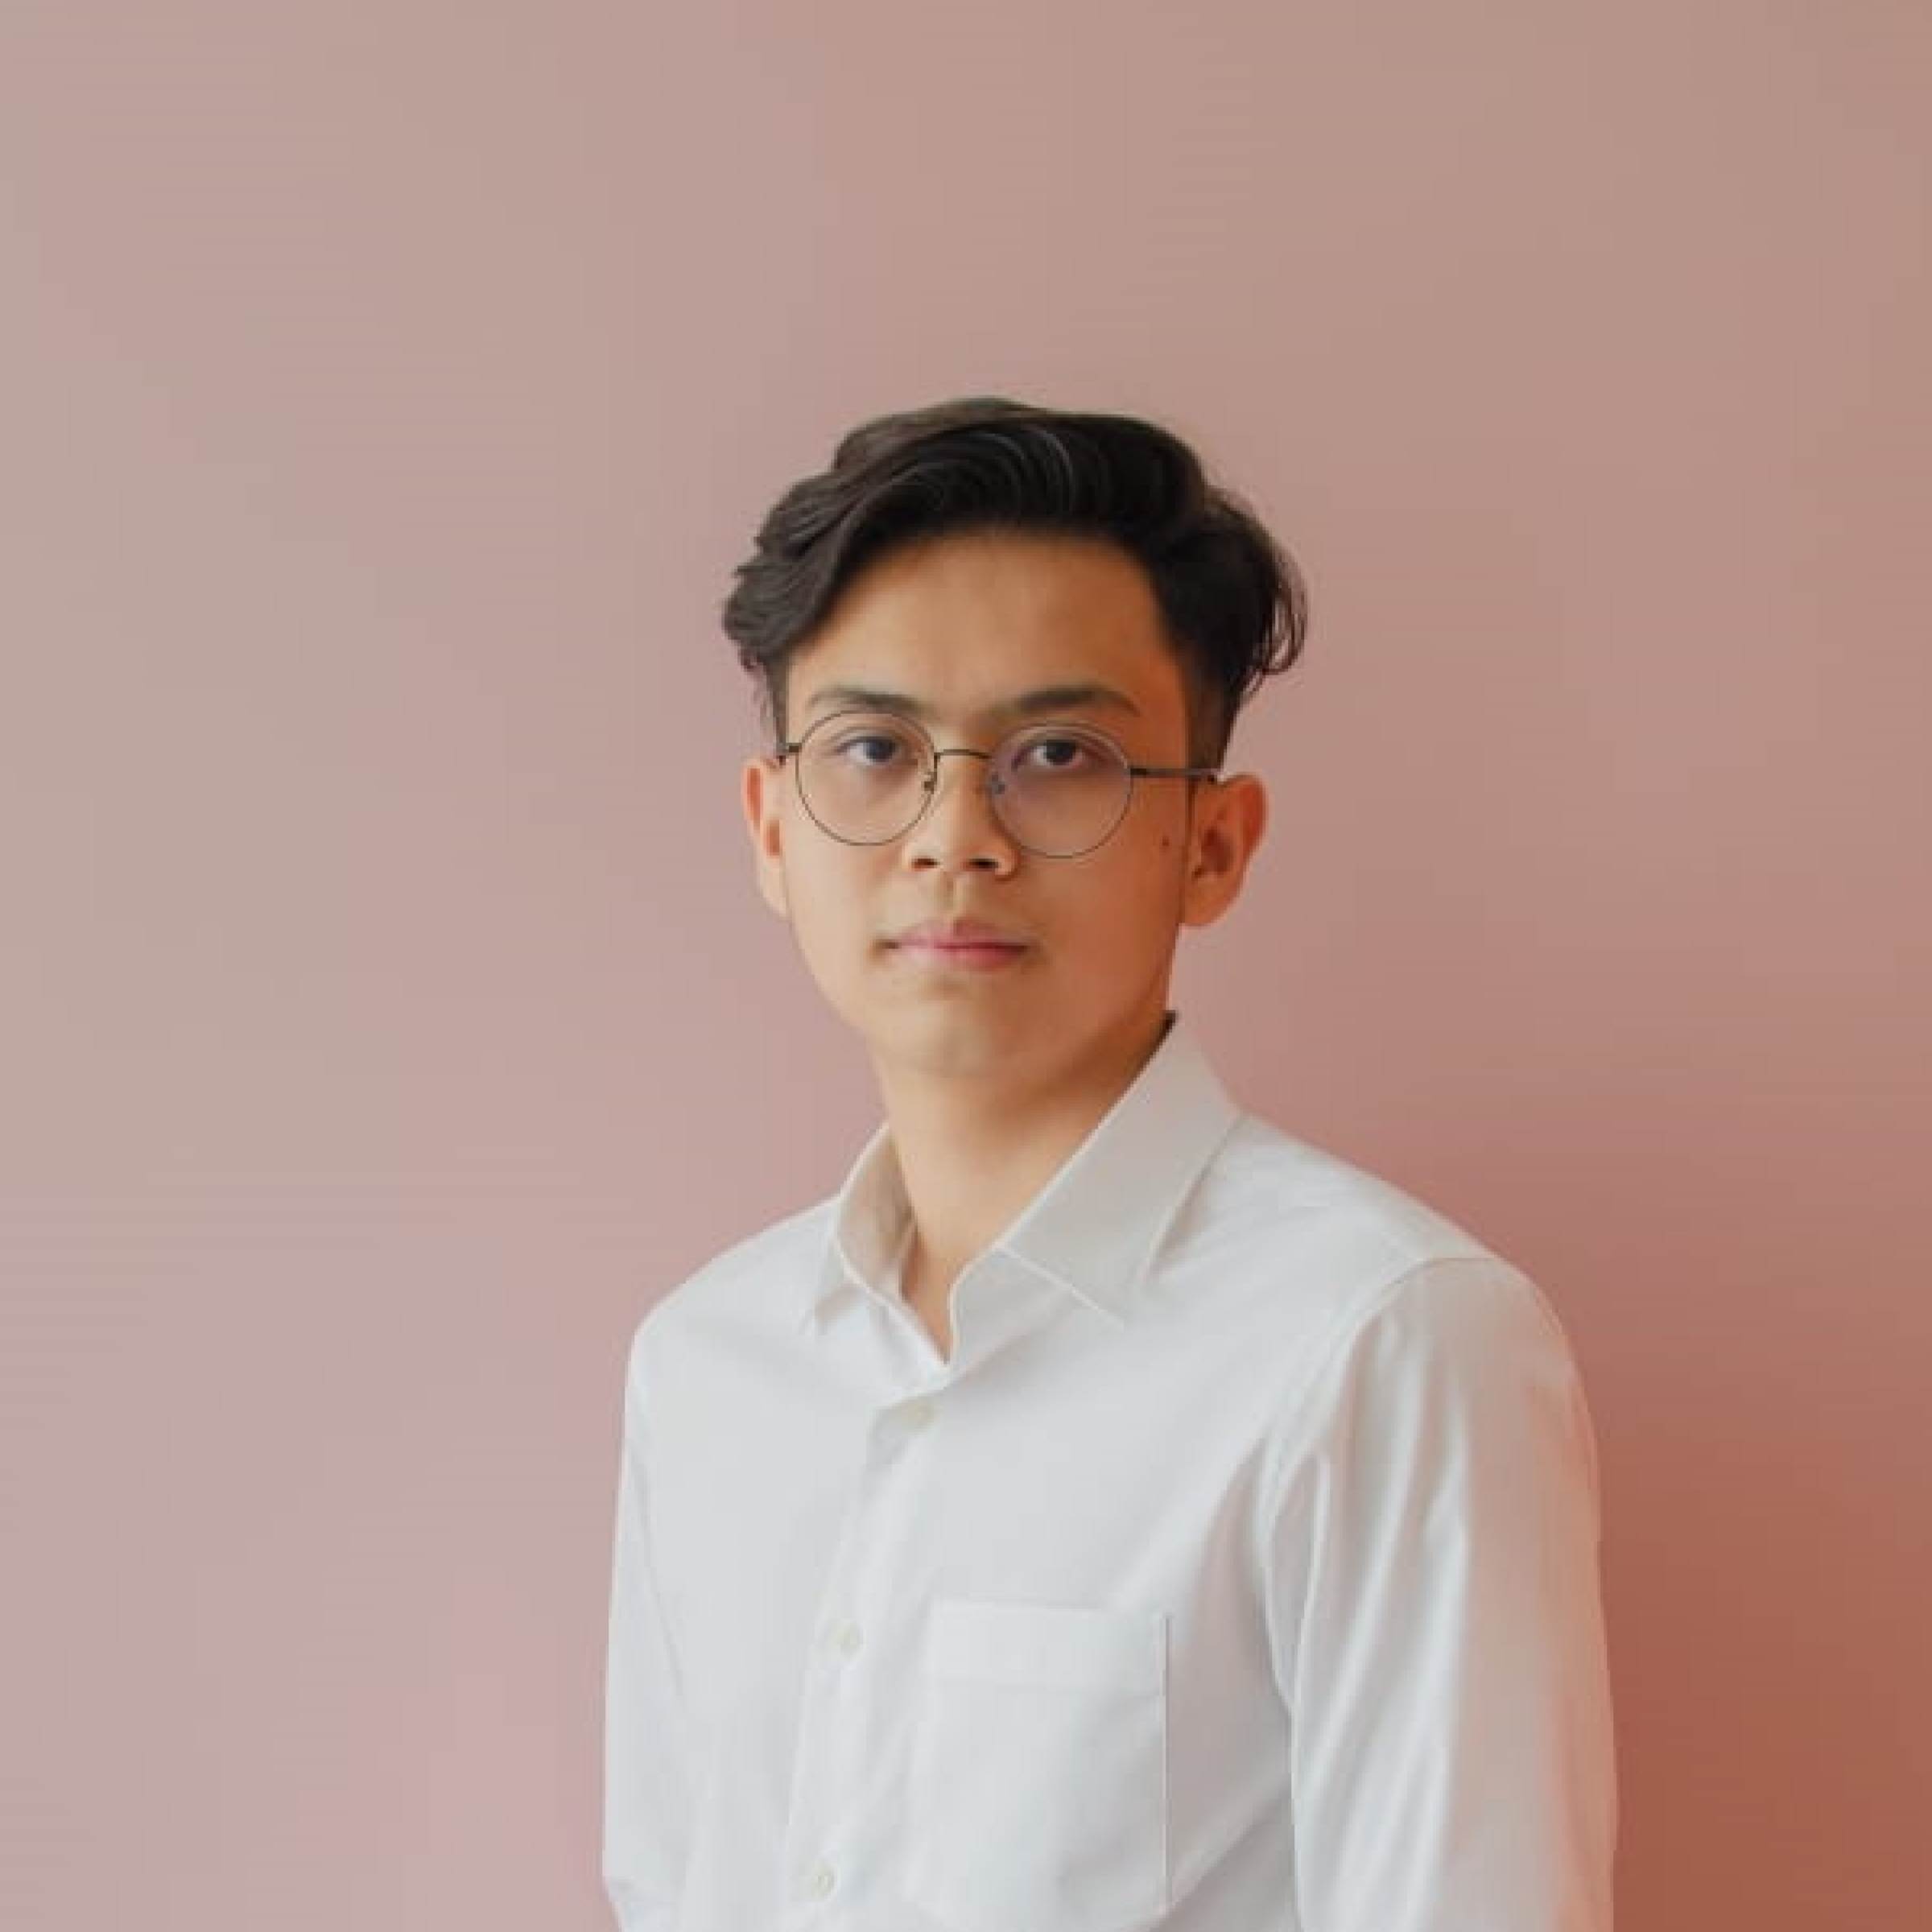
\includegraphics[width=0.3\textwidth]{BiografiPenulis/foto-formal.png}
  \vspace{-4ex}
\end{wrapfigure}

% Ubah kalimat berikut dengan biografi dari mahasiswa
\name{}, atau yang biasa dikenal sebagai Krisna, lahir di Gianyar, Bali pada 8 Juli 2002. Penulis merupakan anak pertama dari tiga bersaudara yang tinggal dan tumbuh besar di Kota Denpasar, Bali. Ketertarikan mendalam penulis di bidang teknologi mengantarkan penulis yang telah menyelesaikan masa sekolah di SMA Negeri 4 Denpasar ke jenjang strata satu di Departemen Teknik Komputer Fakultas Teknologi Elektro dan Informatika Cerdas Institut Teknologi Sepuluh Nopember (ITS) pada tahun 2020.

Penulis merupakan pribadi yang memiliki ketertarikan dalam menjelajahi topik - topik yang berkaitan dengan bidang teknologi secara tekun dan mendalam. Dalam masa kuliah, penulis tertarik dengan topik seperti \emph{Internet Of Things} (IOT), Pengembangan Aplikasi (\emph{Mobile Development}), \emph{Machine Learning}, dan \emph{Computer Vision}. Penulis juga aktif dalam mengembangkan minat dan bakat di luar perkuliahan. Hal ini dibuktikan dengan rekam jejak organisasi dan kepanitian dari penulis seperti Wakil Ketua I Multimedia and Game Development (MAGE) 8, Koordinator Asisten Laboratorium Multimedia dan \emph{Internet Of Things} (IOT), hingga mengikuti program Bangkit Academy 2023. Hingga saat ini penulis terus menekani ketertarikan dan kemampuan yang dimiliki di bidang teknologi, terkhususnya pada bidang Pengembangan Aplikasi (\emph{Mobile Development}) dan \emph{Computer Vision}.

Pada penelitian tugas akhir ini, penulis memilih mengembangkan sistem penerjemah bahasa isyarat Indonesia (BISINDO) yang berfokus pada bidang \emph{Computer Vision}. Keresahan penulis yang memiliki suadara perempuan yang mengalami keterbatasan pendengaran dan berkomunikasi dengan bahasa isyarat menginspirasi dibuatnya tugas akhir ini sebagai bentuk upaya dalam memudahkan komunikasi teman tuli dengan khalayak umum. Bagi pembaca yang memiliki kritik, saran, atau pertanyaan mengenai tugas akhri ini dapat menghubungi penulis melalui surel krisnaerlangga08@gmail.com.

\cleardoublepage
\end{document}
